\newcommand{\scaltex}{Scaltex's Latex Projection}
 
 
\chapter{Einleitung}\label{}
 
\section{Motivation}\label{}
 
Die Erstellung von qualitativ hochwertigen (wissenschaftlichen) Dokumenten ist keine einfache Sache. Das Computerzeitalter konnte zwar schon viel verbessern, aber es gibt noch immer Situationen, in denen die Dokumentenerstellung sehr mühselig werden kann.

 
Zum einen kostet es u.U. sehr viel Zeit, Querreferenzierungen, wie z.B. Verweise im Text auf die korrekten Benummerungen von Abbildungen, im Dokument zu pflegen und konsistent zu halten. Hierfür hat insbesondere LaTeX eine solide Lösung, jedoch stößt man auf der Metaebene, beim LaTeX Code selbst, wieder auf das Problem: Der Autor definiert ein Label und verweist an anderen Stellen darauf. Wird das Label nun irgendwann umbenannt, z.B. weil die Überschrift angepasst wurde, muss es an allen referenzierten Stellen auch umbenannt werden -- manuelles Refactoring des Quelltextes ist notwendig.

 
Zum anderen verstehen die Anwendungen oft nur die Domäne „Dokument“, wenn man z.B. chemische Formeln zeichnen will, müssen diese über externe Ressourcen hinzugefügt werden. Dabei gibt es keinen wirklichen Zugriff mehr auf die Meta-Informationen, die eigentlich durch das Domänenmodell -- die chemische Formel -- mitgeliefert wird. Das kann wiederum zu inkonsistenten Dokumenten führen. Wenn z.B. nachträglich an der chemischen Formel etwas geändert wird und nur die Abbildung vom Benutzer aktualisiert wurde, dann sind u.U. die Verweise (z.B. auf die Masse des chemischen Moleküls) in den beschreibenden Sätzen nicht mehr korrekt. Es fehlt das semantische Verständnis seitens des Dokuments, es weiß also nicht, was die chemische Formel zu bedeuten hat.

 
Zudem liegt hinter keinem derzeit verfassten Dokument ein sauberes \emph{Metamodell}. Das heißt ein Modell, welches eine Struktur vorschreibt, wann welche Dokumentelemente zulässig sind. Eine solche Struktur kann jedoch einen Autor dabei helfen, ein Dokument (wie z.B. ein Bericht der Fraunhofer Gesellschaft) gemäß definierter Vereinbarungen\footnote{~Man kann argumentieren, dass Formatvorlagen von z.B. Microsoft Word auch eine Art Metamodell für ein Dokument sind. Jedoch formalisieren diese nicht, wie eine insgesamte Dokumentklasse korrekt aufgebaut sein soll. Zudem können Autoren sehr leicht, durch manuelle Änderungen, unbeabsichtigt an den Formatvorlagen vorbei arbeiten.} aufzubauen, dabei braucht er kein Wissen über die genaue Vereinbarung und kann dennoch ein formal korrektes Dokument erstellen. Solche Vereinbarungen können z.B. ein Corporate Design oder eine spezielle Aneinanderreihung von Dokumentelementen sein. Weiterhin kann man so ganze Dokumentklassen aus einem solchen Metamodell ableiten: All jene Dokumente, die dem gleichen Metamodell übergeordnet sind, gehören somit ganz formal zur gleichen Dokumentklasse. Beispiele für solche Klassen sind: Masterarbeit, Journal-Paper oder EU-Patent etc.

 
\section{Problemstellung}\label{problemstellung}
 
Aus der Motivation erschließen sich folgende Defizite bzw. Problemfelder in bisherigen Systemen:

 
\begin{enumerate}[(i)]

\item
Mangel an Konsistenz: In bisherigen Textverarbeitungssystemen ist es sehr leicht, Inkostistenzen ins Dokument einzubringen.


\item
Mangel an Domänenwissen: Dokumente „verstehen“ die Konventionen, Konzepte oder Modelle einer Wissenschaft nicht.


\item
Mangel an Semantik: Bedeutungen einzelner Bestandteile eines Dokuments werden oft nicht explizit sichtbar bzw. überhaupt erst verfügbar gemacht.


\item
Mangel an Metamodellierung: Es fehlen\footnote{~Oder gehen nicht weit genug, wie z.B. im Falle von LaTeX. Denn eine Dokumentklasse von LaTeX überprüft nicht, ob eine bestimmte Aneinanderreihung von Dokumentelementen zulässig ist. Beispiel: Sinnloserweise dürfte das Inhaltsverzeichnis auch mitten im Dokument vorkommen. Das heißt, dass die Semantik einer Dokumentklasse von LaTeX nicht unterstützt wird.} formale Vereinbarungen, die eine Dokumentenklasse ausmachen und dem Benutzer bei der Strukturierung helfen.


\end{enumerate}
 
Das wirft die folgende Frage auf: Kann man eine Textverarbeitung erschaffen, welches die o.g. Defizite aufhebt?

 
\section{Stand der Technik}\label{stand-der-technik}
 
Es folgt eine kurze Vorstellung einiger Softwaresysteme die zum erstellen von wissenschaftlichen Dokumenten eingesetzt werden, oder Forschungsprojekte die bestimmte Aspekte der Wissenskonservierung verbessern wollen.

 
\begin{enumerate}

\item Textverarbeitungen
\item Textsatzsysteme
\item SALT
\item OCA
\item Wolfram CDF
\end{enumerate}
 
(1) Sehr weit verbreitet sind Microsoft Word, Apache OpenOffice oder Google Docs. Dabei handelt es sich um WYSIWYG-Editoren für Dokumente. Sie sind für gewöhnlich als Projektionsedtioren für Markup realisiert.

 
(2) Weit verbreitet in den Naturwissenschaften ist TeX bzw. LaTeX (Sammlung an TeX-Makros). Ein Dokument wird in Form von TeX-Quellcode geschrieben und kann zu einer PDF-Datei kompiliert werden. Zur Klasse der Textsatzysteme gehören auch Softwaresysteme wie Adobe InDesign, welche sich stärker den gestalterischen Details widmen, als der inhaltlichen Strukturierung von wissenschaftlichen Texten.

 
(3) Semantically Annotated LaTeX for Scientific Publications ist ein Forschungsprojekt \citep{Groza}, mit dem Ziel LaTeX Code um semantische Annotationen zu erweitern. Es werden Meta-Informationen in die generierten PDFs eingebettet, zur Nutzung durch das Semantic Web.

 
(4) One Click Annotator ist ein Forschungsprojekt \citep{Heese}, welches einen WYSIWYG Web Editor zur entwickelt hat, um Texte um RDFa Annotationen anzureichern.

 
(5) Computable Document Format\footnote{~Wolfram CDF Produktwebseite: http://www.wolfram.com/cdf/} ist ein Dokumentformat für dynamisch generierte, interaktive Inhalte basierend auf der wissensbasierten Wolfram Language. Es handelt sich um ein proprietäres Format, welches zum Betrachten von Dokumenten zumindest den Wolfram Player (oder ein spezielles Browser Plugin) benötigt.

 
\section{Methode}\label{}
 
In erster Linie soll ein Prototyp entwickelt werden, der einen konkreten Lösungsvorschlag für die Problemstellungen aus Abschnitt \ref{problemstellung} vorlegt.

 
Da ein Prototyp wunderbar untersucht werden kann, ist es möglich, theoretische Ideen besser zu veranschaulichen oder überhaupt erst greifbar zu machen. Zudem können unterschiedliche Anwendungsfälle demonstriert werden, um potentiellen Interessenten dieser Technologie Anschauungsmaterial zu liefern und die Praxistauglichkeit der Konzepte zu prüfen. Die Entwicklung eines Protoypen macht bei dieser Masterarbeit also Sinn, da am Prototypen:

 
\begin{itemize}

\item theoretische Konzepte aufgezeigt und empirisch validiert\footnote{~Funktioniert das Konzept richtig?} werden können, und
\item leicht Anwendungsfälle ausprobiert werden können, um die praktische Tauglichkeit der Softwarearchitektur zu verifizieren\footnote{~Verifikation prüft, ob ein System richtig gebaut ist. Oder im Falle von Dokumenten: Ist das Dokument zu einer Spezifikation konform?}.
\end{itemize}
 
\section{Anforderungen}\label{anforderungen-sec}
 
Bei den Anforderungen an den Prototypen kann man schon konkreter in Richtung Implementierung blicken. Hier die Basisanforderungen, um die Problemstellungen zu lösen:

 
Die kleinste Einheit im System ist das Dokumentelement. Beispiele für Dokumentelemente sind: Abschnitte, Absätze, Tabellen, Abbildungen, Fußnoten, etc. Mehr dazu in Abschnitt \ref{dokumentModell}.

 
Dokumentelemente sollen in der Lage sein, konkretes „lebendinges“ Domänenwissen zu beinhalten. Das heißt, dass z.B. eine Zeichnung eines chemischen Moleküls im Hintergrund tatsächlich auf einem formalen Molekülmodell basiert.

 
Reichhaltige Verweisungen unter den Dokumentelementen sollen möglich sein. Das heißt, dass z.B. das formale Modell des Moleküls anderen Dokumentelementen weitere (u.U. berechnete) Informationen bereitstellen kann.

 
Ein Metamodell definiert die im Dokument vorkommenden Dokumentelemente formal. Das Dokument selbst soll folglich als Modell (Instanz) aufgefasst werden.

 
Um die Software benutzbar zu machen, gibt es folgende Nebenbedingungen:

 
\begin{itemize}

\item Es soll ein reaktives System sein, welches sofort auf Eingaben des Benutzers bzw. Veränderungen des Systemzustands reagiert.
\item Es soll also ein „lebendiges“ Dokument werden, d.h. es sollen keine (spürbaren) Kompilierzeiten, um das Dokument zu erstellen, entstehen.
\item Da es in wissenschaftlichen Dokumenten meist zu komplizierten Verweisungen kommt, müssen diese in jedem Fall konsistent gehalten werden. Es soll daher das Problem des manuellen Refactoring abgefedert werden.
\item Es soll ein Einheimischer des WWW werden, d.h. Web Standards sind das Ausgabeformat. Sie übernehmen das Setzen des Dokuments, bieten dem Benutzer eine Editierschnittstelle, ermöglichen Kollaboration und bieten eine ubiquitäre Wissensrepräsentation.
\end{itemize}
 
Durch einige dieser Anforderungen zielen implizit auf die Implementierung eines Projektionseditors und haben sogar Potential für ein „Dokument Query Interface“. Das heißt das Dokument im Ganzen oder ein Dokumentelement im Speziellen, kann befragt werden einen bestimmten Sachverhalt herauszufinden. Beispielsweise können so komfortabel alle Abschnitte nach ihrer Benummerung abgefragt werden.

 
\section{Idee}\label{}
 
Im Vordergrund stand die Idee, meine Bachelorarbeit \citep{Hodapp} so weiter zu entwickeln, dass Dokumente in einem Projektionseditor (mehr dazu in Abschnitt \ref{Projektionseditoren-sec}) verfasst werden können und mit domänenspezifischen Dokumentelementen interagiert werden kann. Die Bachelorarbeit hat sich damit beschäftigt, (1) ein Dokument im Browser zu layouten und zu paginieren und (2) eine interne DSL für Dokumente zu entwickeln, welche eine Datenstruktur zur Verarbeitung für den Layouter ausgibt.

 
In diesem Kapitel wird also kurz die prinzipielle Idee umrissen, wie man die Problemstellung unter den gegebenen Anforderungen lösen könnte.

 
Grundsatz der Idee ist, dass jedes Dokumentelement auf einen Aktor abgebildet wird. Ein Aktor kann Nachrichten senden und empfangen, zudem kapselt er einen Zustand und ein Verhalten.

 
Aktoren können, ebenso wie ein Dokument, hierarchisch angeordnet werden. Das heißt ein Aktor kann Kinder und Geschwister haben. Diese Anordnung ergibt eine baumartige Graphenstruktur, worin ein Aktor einem Knoten entspricht und eine Referenz\footnote{~Über eine solche Aktor Referenz können Nachrichten an andere Aktoren übermittelt werden.} auf einen anderen Aktor einer Kante.

 
Diese Baumstruktur kann als abstrakter Syntaxbaum (AST) der Dokumentenstruktur aufgefasst werden. Der AST kann als ein Modell für ein Dokument aufgefasst werden. Dies wird auf Abbildung \ref{idee} veranschaulicht. Zudem kann mit Hilfe eines AST ein Projektionseditor (siehe Abschnitt \ref{Projektionseditoren-sec}) umgesetzt werden.

 
Der hier mit den Aktoren umgesetzte AST könnte als „reaktiver AST“\footnote{~„Merriam-Webster definiert reaktiv als ‚immer bereit auf ein Stimulus zu reagieren‘, z.B. sind Komponenten immer ‚aktiv‘ und jederzeit bereit auf Ereignisse zu reagieren.“ Frei übersetzt aus dem Reactive Manifesto: http://www.reactivemanifesto.org/} bezeichnet werden, da er dank der Aktoren (quasi gratis) besondere Eigenschaften erhält:

 
\begin{itemize}

\item Verteilbarkeit, Fehlertoleranz und massive Parallelität. Der AST kann z.B. auf ein Cluster gebracht werden, z.B. zur Kompilierung des Dokuments in „der Cloud“; Anwendung von MapReduce auf Dokument oder Dokumentenserie; Jeder Aktor ist autonom, d.h. z.B. asynchrone Datanbankzugriffe oder schnelle Reaktionszeiten auf Änderungen.
\item Möglichkeit zum Query Interface ausgebaut zu werden. Das Dokument bzw. Dokumentelement kann auf Nachrichten reagieren. Beispielsweise zur Aggregation neuer Informationen.
\item Möglichkeit mit anderen (Aktoren-) Systemen (z.B. Dokumenten) zu interagieren. Beispielsweise via Akka Remoting Protokoll oder Anbindung an REST-Schnittstellen.
\end{itemize}
 
\begin{figure}[h!]
\centering
\advance\leftskip-2.5cm
\fbox{ 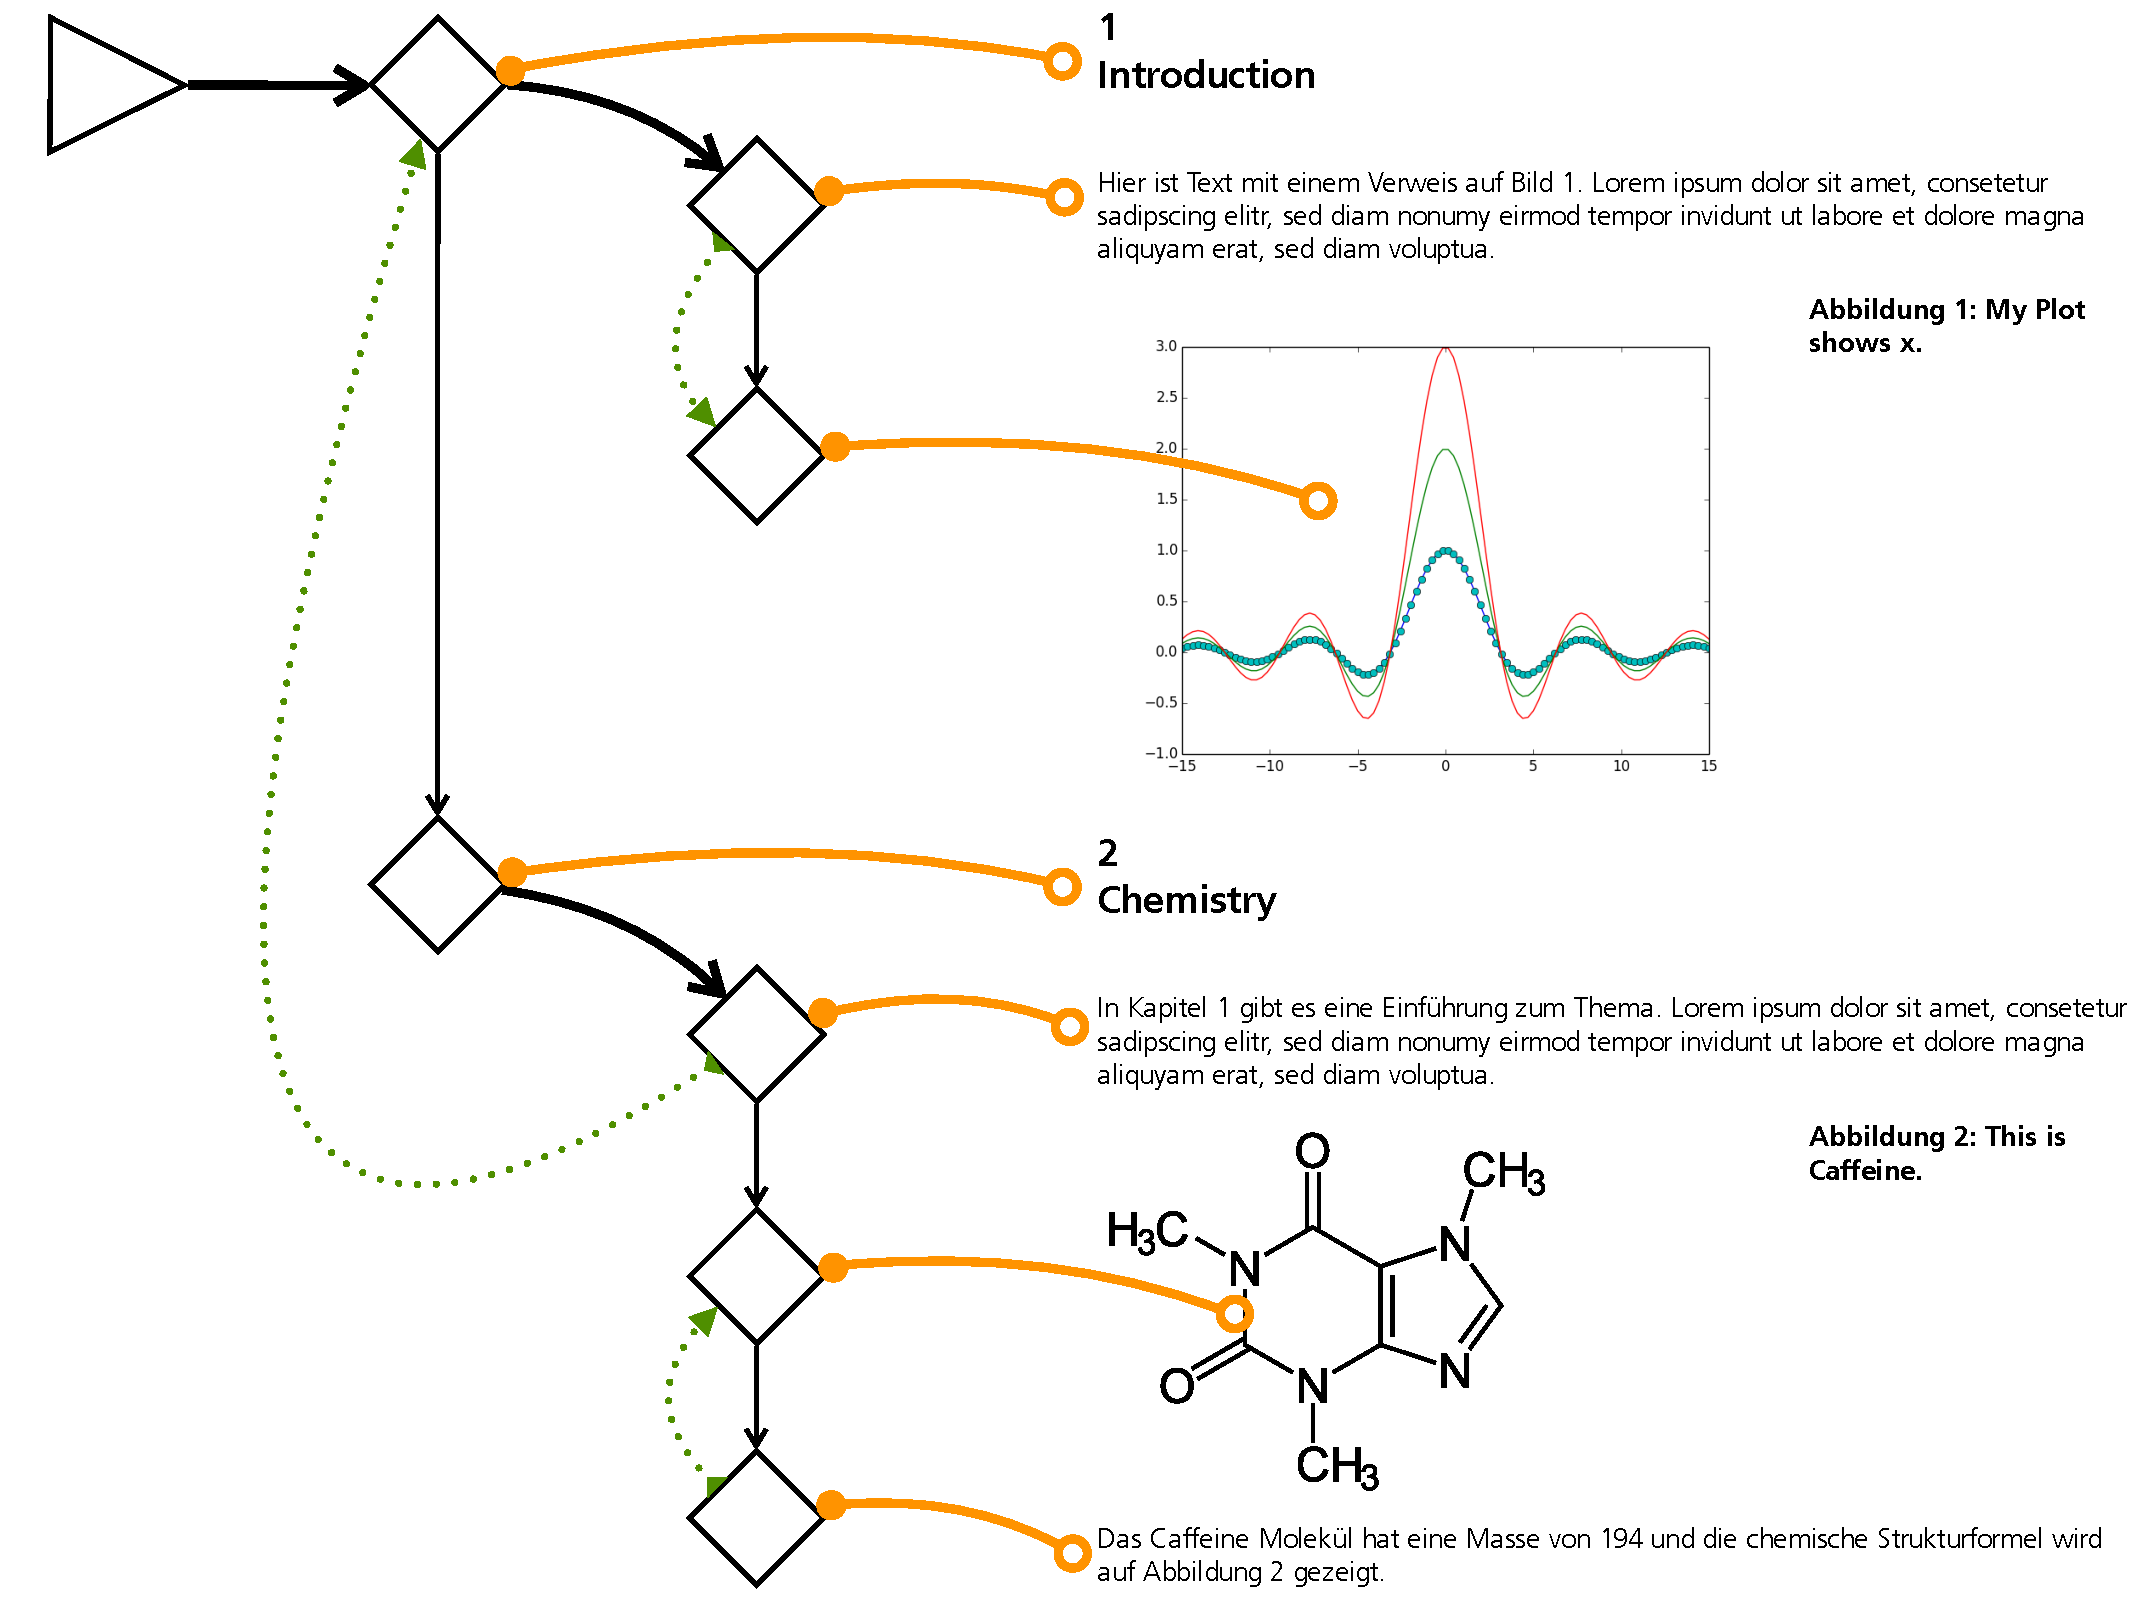
\includegraphics[width=1.45\textwidth]{figures/idee.svg.pdf} }
\caption{ Modell für ein Dokument. Jeder Aktor (Raute) repräsentiert ein Dokumentelement. Die Aktoren kennen sich (graue Pfeile) und spannen somit einen Graphen auf. Die Aktoren können Nachrichten (grüne Pfeile) austauschen, z.B. um Benummerungen aufzulösen. }\label{idee}
\end{figure}
 
\section{Szenario}\label{}
 
Ein motivierendes Szenario ist auf Abbildung \ref{szenario} visualisiert. Hierbei kann der Autor zunächst sein Dokument in einer abstrakteren Ansicht editieren. Dadurch werden die Beziehungen, und deren Bedeutungen, zwischen den einzelnen Dokumentelementen klar. Zudem kann er im Falle des Moleküls auch auf weitere Informationen, die das Molekül-Dokumentelement anbietet, zugreifen. Das hilft den Autor dabei, sein Dokument konsistent zu halten.

 
\begin{figure}[h!]
\centering
\advance\leftskip-2.5cm
\fbox{ 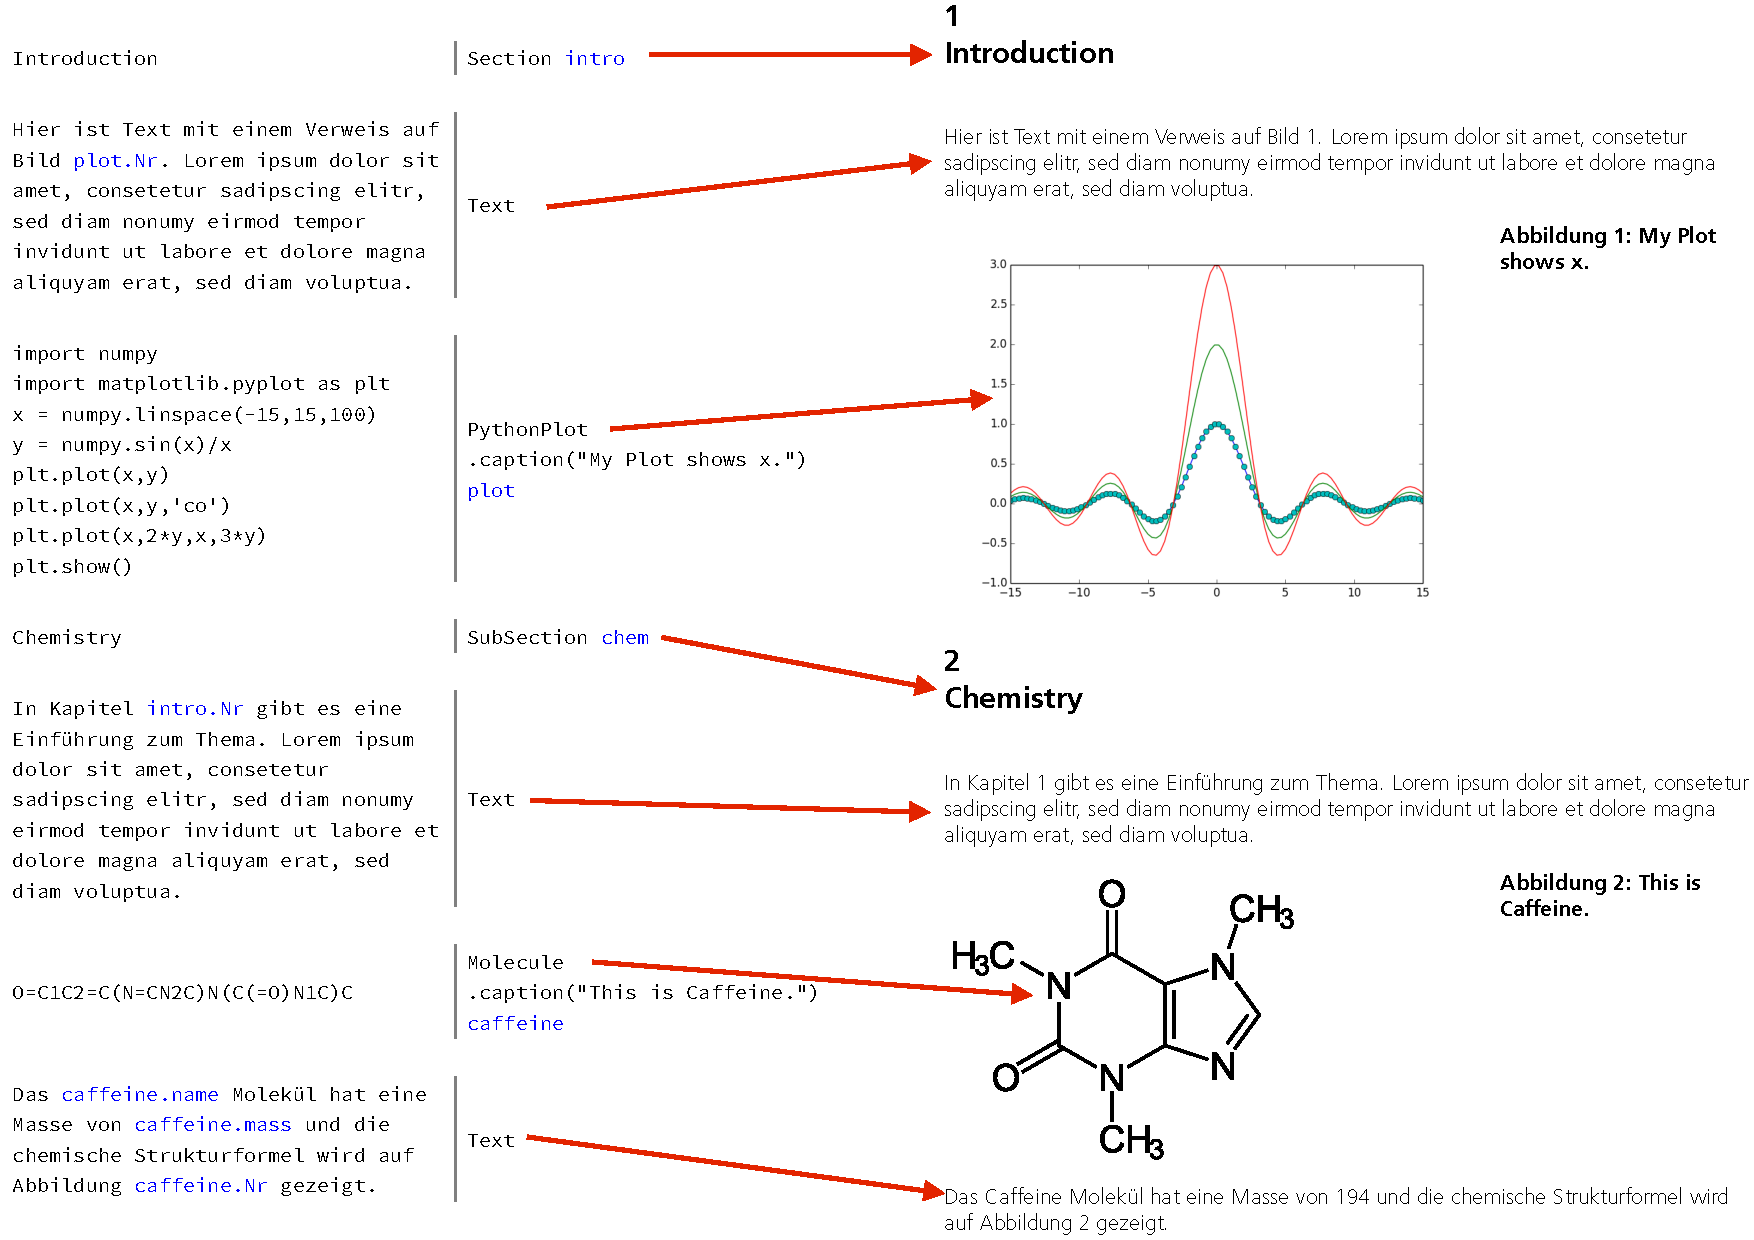
\includegraphics[width=1.45\textwidth]{figures/szenario.svg.pdf} }
\caption{ Motivierendes Szenario. Auf der linken Seite ist die Editier-Ansicht zu sehen, dort werden die einzelnen Dokumentelemente und ihre Beziehungen (Verweise untereinander) ersichtlich. Die Verweise zwischen den Dokumentelementen sind blau markiert. Auf der rechten Seite ist die durch ein Satzsystem gesetzte Ansicht, welche aus der Editier-Ansicht hervorgeht. }\label{szenario}
\end{figure}
 
\section{Fragen von wissenschaftlichem Interesse}\label{wiss-fragen}
 
Bereiche in denen (wiss.) Fragestellungen durch den Prototypen beantwortet werden können:

 
\begin{itemize}

\item
Modellgetriebene Software-Entwicklung: Ist es sinnvoll Dokumente als Modell aufzufassen? Wie könnte eine sinnvolle Modellierung von Dokumenten aussehen? Gibt es ein gemeinsames Metamodell?


\item
Programmiersprachen, Compilerbau: Kann ein Aktorsystem verwendet werden, um einen abstrakten Syntaxbaum zu implementieren? Taugt dieser abstrakte Syntaxbaum als sinnvolle Architekturgrundlage für einen Projektionseditor, und damit auch als Code Generator?


\item
Knowledge Engineering / Management; Semantik, Ontologie: Brauchen wir mehr explizite Semantik innerhalb von Dokumenten? Ergeben sich Vorteile, wenn diese Semantik direkt vom Autor transportiert wird? Ist es möglich, dass sich Dokumente zu einem gewissen Grad selbst verifizieren\footnote{~Verifikation prüft, ob ein System richtig gebaut ist. Oder im Falle von Dokumenten: Ist das Dokument zu einer Spezifikation konform?} und damit konsistenter machen?


\item
Bibliotheks- und Informationswissenschaften: Gibt es eine allgemeingültige Taxonomie für wiss. Publikationen?


\end{itemize}
 
\chapter{Theorie der Dokumente}\label{}
 
In diesem Kapitel wird überlegt, was der modelltheoretische Hintergrund von (wiss.) Dokumenten im Allgemeinen ist. Und wie sich domänenspezifische Inhalte darauf auswirken. Die hier erarbeiteten Theorien sind das Destillat dessen, was aus dem Prototyp gelernt wurde.

 
Zunächst wird der Modellbegriff erläutert, um anhand dessen ein geeignetes Modell für Dokumente abzuleiten. Daraus folgt, dass eine natürliche Repräsentation der Graph aus der Graphentheorie ist (siehe Abschnitt \ref{modellbegriff-sec}). Eine spezielle Form von Graphen ist der abstrakte Syntaxbaum, welcher in der Informatik als abstrakte Repräsentation für Programmcode dient (siehe Abschnitt \ref{ast-sec}). Auf diese Weise kann ein Dokument auch als Programm aufgefasst und verarbeitet werden. Projektionseditoren geben einem Programmierer (oder hier Autor) die Möglichkeit, direkt einen abstrakten Syntaxbaum (grafisch) zu editieren (siehe Abschnitt \ref{Projektionseditoren-sec}).

 
Um ein Modell formal besser fassbar zu machen, ist es dienlich ein Metamodell darüber zu stellen (siehe Abschnitt \ref{metamodellbegriff-sec}). Das Metamodell beschreibt aus welchen Entitäten und Beziehungen ein konformes Modell besteht. Begriffe aus der Semiotik, der allgemeinen Lehre der Sprachen, lassen erkennen, dass jedes einzelne Dokumentelement wiederum ein Modell einer spezifischen Domäne kapselt (siehe Abschnitt \ref{semiotik-sec}). Der innere Aufbau von wissenschaftlichen Dokumenten kann in eine Taxonomie eingeordnet werden. So können verschiedene Typen von Dokumentelementen hierarchisch angeordnet werden. Diese Dokumentelement-Typen können als Matrix angeordnet werden, dort lassen sich erlaubte Verschachtelungen bzw. Aneinanderreihungen der Dokumentelemente formal spezifizieren. Mehr dazu in Abschnitt \ref{taxonomie-sec}.

 
\section{Modellbegriff}\label{modellbegriff-sec}
 
\begin{quote}
 Modellierung ist das uns angeborene Verfahren, das komplexe Universum auf eine überschaubare Welt zu reduzieren. Indem wir sichtbare und unsichtbare Phänomene auf Begriffe abbilden und nur noch mit diesen umgehen, wird die Gesamtzahl der zu betrachtenden Gegenstände beherrschbar[...] \citep[S.~7]{Ludewig}
\end{quote}
 
Gerade auch in der Wissenschaft spielen Modelle die zentrale Rolle, denn „Das Resultat einer Forschung ist in jedem Falle ein Modell, eine Theorie.“ \citep[S.~8]{Ludewig} Warum sollte man also nicht den Weg ganz konsequent gehen, und ebenfalls die wissenschaftliche Dokumentation selbst als Modellierung betrachten? Warum sollte das Dokument selbst nicht Modelle aus einer Wissenschaft bereitstellen? Das heißt, dass eine Wissenschaftlerin bzw. ein Wissenschaftler seine Modelle direkt im Dokument verwenden kann?

 
\subsection{Modellmerkmale}\label{modellmerkmale}
 
In \citep[S.~9]{Ludewig} ist eine griffige Zusammenfassung der drei zwingenden Merkmale die nach \citep{Stachowiak} vorliegen müssen, um als Modell zu gelten, aufgeführt. Diese werden hier sinngemäß zusammengefasst und durch Abbildung \ref{modell} veranschaulicht:

 
\begin{enumerate}

\item Abbildung: Ein Modell ist immer ein Abbild eines Originals. Die Abbilder können beliebig geartet sein, d.h. das Modell muss dem Original äußerlich nicht ähneln. Das Original auf welches sich das Modell bezieht, kann neben natürlichen Objekten auch künstlich, geplant oder vermutet sein.
\item Verkürzung: Ein Modell erfasst nicht alle Merkmale des Originals. Durch Verkürzung fallen Attribute weg, diese werden übergangen oder präteriert genannt. Das Modell kann jedoch zusätzliche Attribute haben, die so im Original nicht vorkommen, diese werden überflüssig oder abundant genannt.
\item Pragmatismus: Ein Modell muss einen Sinn haben, um unter bestimmten Fragestellungen das Original ersetzen können. Das heißt, es wird das Modell statt des Originals untersucht, um daran die Nützlichkeit für eine Zielgruppe (für wen, wann, wozu?) festzustellen.
\end{enumerate}
 
\begin{figure}[h!]
\centering
\advance\leftskip-2.5cm
\fbox{ 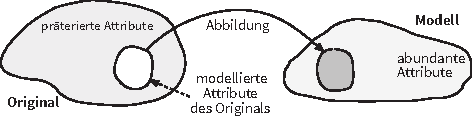
\includegraphics[width=1.45\textwidth]{figures/modell.svg.pdf} }
\caption{ Schematische Zeichnung der Original-Modell-Beziehung. Entnommen aus (Ludewig, 2002, S. 9). }\label{modell}
\end{figure}
 
\subsection{Modell eines Dokuments}\label{dokumentModell}
 
Bevor ein passendes Modell für Dokumente gefunden werden kann, muss man sich bewusst sein, dass es dem Abbildungsmerkmal, Verkürzungsmerkmal und dem pragmatischen Merkmal, welche in Kapitel \ref{modellmerkmale} beschrieben sind, genügen muss.

 
Das Original ist in jedem Fall ein gesetztes statisches Dokument, z.B. ein auf Papier gedrucktes Buch oder ein (wiss.) Bericht im PDF-Dateiformat.

 
Dort interessieren uns als Autor in erster Linie aber nur die wirklich inhaltstragenden Attribute des Originals. Auf einer höheren Abstraktionsebene entsprechen diese den Dokumentelementen, wie z.B. Abschnitte, Absätze, Abbildungen etc. Im Falle von z.B. Abschnitten ist nur der Titel maßgeblich, die Benummerung kann auch erst später (durch Berechnung) hinzugefügt werden. Das heißt hier wäre der Titel ein Attribut welches vom Original in das Modell abgebildet wird; die Benummerung wäre jedoch ein abudantes Attribut welches erst innerhalb des Modells erstellt wird. Layoutinformationen, Schriftarten oder Papiersorte spielen dafür keine Rolle und können somit weggelassen werden.

 
Wenn der Autor an seinem Dokument arbeitet, dann stets über das Modell, wo er sich ausschließlich auf die Dokumentelemente konzentrieren kann. Das Modell kann präskriptiv sein, d.h. aus dem Modell kann wieder ein Original entspringen.

 
Hier wird der abstrakte Syntaxbaum als Modell für das Dokument dienen, indem jedes Dokumentelement als ein Knoten des abstrakten Syntaxbaum aufgefasst wird. Mehr zum abstrakten Syntaxbaum in Abschnitt \ref{ast-sec}. Wie man sich eine Abbildung von einem Dokument auf einen abstrakten Syntaxbaum vorstellen kann, ist auf Abbildung \ref{idee} visualisiert.

 
\subsubsection{Beweis}\label{}

 
\begin{itemize}

\item Abbildungsmerkmal: Der abstrakte Syntaxbaum („das Modell“) ist z.B. ein Abbild eines gedruckten Buches, da Dokumentelemente als Knoten im Syntaxbaum vorkommen.
\item Verkürzungsmerkmal: Nur die Attribute aus dem Original werden modelliert, die den maßgeblichen Inhalt des Dokuments transportieren (z.B. Text). Diese Inhalte werden als Dokumentelemente modelliert.
\item Pragmatischen Merkmal: Der Autor greift auf das Modell zurück, um daran die herausgelösten und essentiellen Dokumentelemente zu untersuchen bzw. zu manipulieren.
\end{itemize}
 
Alle Bedingungen für den Modellbegriff nach \citep{Stachowiak} sind erfüllt. ■

 
\section{Abstrakter Syntaxbaum}\label{ast-sec}
 
In diesem Abschnitt werden die prinzipiellen Eigenschaften von abstrakten Syntaxbäumen, kurz AST, beschrieben.

 
Laut \citep{Aho} ist der AST eine Datenstruktur, die von einem Übersetzer als Zwischenrepräsentation eines Quellcodes generiert wird. Er repräsentiert die hierarchische syntaktische Struktur eines Programms. Aus einer solchen Zwischenrepräsentation wird schlussendlich das Zielprogramm generiert.

 
Wärend der Syntaxanalyse (parsing) werden Syntaxbaum-Knoten erstellt, welche wiederum signifikate Programmkonstrukte repräsentieren. Die Kinder des Knoten sind die bedeutungstragenden Komponenten des Konstrukts. Beispielsweise (s. Abb. \ref{ast}): Gegeben ist ein AST für einen Ausdruck (expression), dann repräsentiert jeder innere Knoten einen Operator und die Kinder des Knoten sind die Operanden. Man beachte jedoch, dass Syntaxbäume für beliebige Konstrukte erstellt werden können und nicht auf Ausdrücke beschränkt sind. Jedes Konstrukt ist durch einen Knoten repräsentiert, dessen Kinder semantisch bedeutungsvolle Komponenten des Konstruktes sind. Durch fortschreitende Analyse können Informationen vom Übersetzer zu den Knoten als Attribute hinzugefügt werden. (ebd.)

 
\begin{figure}[h!]
\centering
\advance\leftskip-2.5cm
\fbox{ 
\includegraphics[width=1.45\textwidth]{figures/ast.svg.pdf} }
\caption{ Abstrakter Syntaxbaum für den Ausdruck 9-5+2. Entnommen aus (Aho, 2007, S. 70). }\label{ast}
\end{figure}
 
\subsection{Allgemeine Implementierung}\label{}
 
Wenn ein Operator, also ein innerer Knoten, beliebig viele Operanden, also Kinder des Knoten, haben darf, spricht man von einem n-stelligen bzw. n-ary AST. \citep{Edwards} Eine solche Struktur ist auf Grafik \ref{astimpl} veranschaulicht.

 
\begin{figure}[h!]
\centering
\advance\leftskip-2.5cm
\fbox{ 
\includegraphics[width=1.45\textwidth]{figures/astimpl.svg.pdf} }
\caption{ Generellste Implementierung eines AST. Entnommen aus (Edwards, 2003). }\label{astimpl}
\end{figure}
 
\subsection{Übertragung auf den Prototypen}\label{}
 
Die zentrale Struktur des hier vorgestellten Prototyps ist ebenfalls ein abstrakter Syntaxbaum. Das ist legitim, da Syntaxbäume beliebige Konstrukte repräsentieren können. Jedoch handelt es sich nicht ausschließlich um eine Datenstruktur, da Aktoren als die Baum-Knoten fungieren und Aktoren neben der reinen Datenhaltung auch auf Nachrichten reagieren können. Man könnte quasi davon sprechen, dass der abstrakte Syntaxbaum in dem hier vorgestellten System eine „lebendige Datenstruktur“ ist. Das kann dahingehend von Vorteil sein, da der AST dadurch befähigt ist, selbstständig eine Analysephase durchzuführen.

 
In einer solche Analysephase werden u.U. weitere Informationen zu den Knoten hinzugefügt. Beispiel: Eine Hierarchie von Kapiteln kann während der Analyse die jeweils richtige Benummerung ermitteln und jeder Aktor (also Knoten) speichert sich diese Benummerung intern als Attribut ab.

 
Der Basis Aktor aus Abbildung \ref{metamodell} entspricht quasi 1:1 der generellen Implementierung aus Abbildung \ref{astimpl}. Das hier vorgestellte Metamodell (s. Abschnitt \ref{metamodell_dokument}) beschreibt auch eindeutig einen AST. Die Knoten entsprechen den Aktoren, welche wiederum die einzelnen Dokumentelemente des Dokuments repräsentieren. Dieser AST, gesehen als Programmsyntax, beschreibt somit den hierarchischen Aufbau des Dokuments.

 
Die inneren Knoten, die z.B. Operatoren repräsentieren können, entsprechen hier hierarchiebildenden oder gliedernden Elementen. Diese können (müssen aber nicht) im Dokument sichtbar sein. Beispiele dafür sind z.B. Kapitel, Abschnitte oder die Titelei. Die Kinder dieser Knoten sind bedeutungsvolle Komponenten für den Knoten dahingehend, dass sie entweder weiter die Hierarchie des Dokuments aufspannen und somit das Dokument weiter gliedern oder im Falle von Blättern, die eigentlich inhaltstragenden Elemente sind. Die Blätter müssen auf jeden Fall im Dokument sichtbar sein. Beispiele dafür sind z.B. Absätze oder Abbildungen.

 
\section{Projektionseditoren}\label{Projektionseditoren-sec}
 
Für gewöhnlich arbeiten Programmierer mit Quellcode-Editoren, das heißt es werden Schriftzeichen direkt in eine Datei geschrieben. Diese Schriftzeichen bilden die konkrete Syntax einer Programmiersprache. Der Editor kann das arbeiten mit Quellcode erleichtern, indem er z.B. die Schlüsselwörter einer Programmiersprache farbig hervorhebt. Um ein Programm aus der Datei zu generieren, muss ein Übersetzer zunächst eine Syntaxanalyse (parsing) durchführen. Bei dieser Analyse wird die Datei in Wörter, die es in der Programmiersprache gibt, zerhackt. Anhand dieser Wörter kann der Übersetzer z.B. eine Baumstruktur aufbauen, um die syntaktische Korrektheit des Programms zu prüfen. Das heißt der Übersetzer kann anhand es Baumes feststellen, ob es sich um ein korrektes Programm handelt. Dann kann aus der, als korrekt befundenen, Baumstruktur der eigentliche Maschinencode erzeugt werden.

 
Projektionseditoren gehen anders vor: Der Editor arbeitet direkt auf dem abstrakten Syntaxbaum (s. Abschnitt \ref{ast-sec}), d.h. der Programmierer editiert nicht mehr eine Datei die durch den Übersetzer in eine Baumstruktur umgewandelt wird, sondern seine editier-Operationen verändern direkt die Baumstruktur des Programms. \citep[S.~68]{Voelter} Nun kann aus der abstrakten Syntax (entspricht der Baumstruktur) eine Variation an konkreten Syntaxen erstellt werden, die sogenannten Projektionen. Diese Projektionen können wieder textuell sein, aber auch grafisch -- jedoch sind diese in ihrer Darstellung deutlich flexibler als bei parserbasierten Editoren. Eine kurze schematische Grafik (Abb. \ref{parserprojectional}) verdeutlicht den Unterschied zwischen Quellcode-Editoren und Projektionseditoren.

 
Im englischen\footnote{~Projectional Editing in Wikipedia: \url{http://en.wikipedia.org/wiki/Projectional\_editor}} Sprachraum gibt es mehrere Bezeichnungen: structure editor, structured editor oder projectional editor. Man kann diese mit Struktureditor oder Projetkionseditor übersetzten.

 
Die Idee von Projektionseditoren ist nicht neu, bereits 1971 hat Wilfred J. Hansen ein System entwickelt, welches auf solch einem Ansatz beruht. Jedoch haben sich zur damaligen Zeit diese Editor-Formen nicht durchgesetzt, wegen der unzureichenden Benutzerfreundlichkeit. \citep[S.~91]{Gomolka} In heutigen Zeiten (insbesondere mit den fortgeschrittenen Web Standards) sollte es aber möglich sein, einen benutzerfreundlichen Projektionseditor zu bauen, der die Produktivität und den Komfort erhöht.

 
\begin{figure}[h!]
\centering
\advance\leftskip-2.5cm
\fbox{ 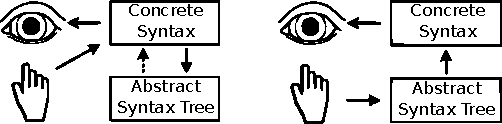
\includegraphics[width=1.45\textwidth]{figures/parserprojectional.svg.pdf} }
\caption{ Parserbasierte Editierung / Quellcode-Edior (links) verglichen mit projektionsbasierter Editierung / Projektionseditor (rechts). Im parserbasierten Ansatz sieht und bearbeitet der Programmierer die konkrete Syntax eines Programms. Ein Übersetzer gewinnt aus der konkreten Syntax einen AST. Beim projektionsbasierten Ansatz sieht der Programmierer eine (von vielen) konkrete Syntax, und bearbeitet jedoch unmittelbar den AST. Im Allgemeinen kann aus dem AST eine konkrete Syntax gewonnen werden, das kann z.B. Quellcode einer Programmiersprache sein, aber auch direkt Maschinencode. Grafiken aus (Voelter, 2013, S. 68) entnommen. }\label{parserprojectional}
\end{figure}
 
\subsection{Übertragung auf den Prototypen}\label{}
 
Der hier vorgestellte Prototyp ist augenscheinlich ein Projektionseditor. Sein Basiskonzept ist Dokumente als ein Modell zu sehen. Und das Modell eines Dokuments erscheint hier in Form eines abstrakten Syntaxbaumes. (s. Kapitel \ref{dokumentModell}) Der Editor arbeitet also „per Design“ als Projektionseditor. Die Projektionen entsprechen einfachen HTML-Templates, die jedem Dokumentelement sein Aussehen verleihen. Werden die Templates ausgetauscht, können ganz andere Repräsentationen bzw. konkrete Syntaxen des vorliegenden abstrakten Syntaxbaumes möglich sein. Beispielsweise kann der Prototyp aktuell neben der „gesetzten“ Web-Ansicht auch noch LaTeX-Code als Projektion anbieten -- das gleiche Dokument in verschiedenen Ansichten oder Projektionen.

 
\section{Metamodellbegriff}\label{metamodellbegriff-sec}
 
\begin{quote}
 Werden Modelle und Modellbildung selbst zum Gegenstand der Modellierung, so spricht man von Metamodellen. \citep[S.~1]{Strahringer}
\end{quote}
 
\citep{Strahringer} hat versucht den Metamodellbegriff anhand der Sprachstufentheorie der Logik, durch Übertragung auf die Modellierungswelt, zu prägen. \citep[S.~1]{Strahringer} erklärt, dass nach \citep{Buehler} die Sprache drei Funktionen leistet: (1) Darstellung von Sachverhalten, (2) Appell zur Verhaltenssteuerung und (3) Ausdruck von Gefühlen. Für den Metamodellbegriff ist jedoch nur die Darstellungsfunktion interessant. Sprache stellt „ein mögliches Instrument zur Darstellung von Modellen“ (ebd.) dar.

 
\citep[S.~1]{Strahringer} führt fort, dass in der Logik üblicherweise zwischen Objektsprache und Metasprache unterschieden wird. Die Objektsprache ist Gegenstand der Untersuchung. In der Metasprache erfolgt die Untersuchung. Da die Metasprache selbst auch wieder Gegenstand einer Untersuchung werden kann, ist dieses Prinzip rekursiv anwendbar. Um endlose Rekursion zu vermeiden, sollte als oberstes Glied der Kette ein selbstbeschreibendes Metamodell stehen. Beispielsweise die Meta Object Facility (MOF) der OMG\footnote{~Die OMG (Object Management Group) hat MOF (Meta Object Facility) als Standard (ISO/IEC 19508) veröffentlicht. } geht so vor, um endlose Meta-Rekursionen zu vermeiden.

 
Wird „die Sprachstufentheorie auf die Modellbildung [...] übertragen, so“ (ebd.) kann im einfachsten Fall ein Metamodell „als ein Modell eines Modells“ (ebd.) beschrieben werden.

 
\begin{quote}
 Wird die Objektsprache, in der das Modell der untersten Stufe formuliert ist, abgebildet in einem Beschreibungsmodell, so handelt es sich um ein Metamodell. \citep[S.~3]{Strahringer}
\end{quote}
 
„Beschreibungsmodelle dienen der systematischen Beschreibung des betrachteten Gegenstandsbereiches und bestehen aus ausschließlich deskriptiven Satzsystemen.“ Das heißt, ein Beschreibungsmodell ist ein Modell welches so formuliert wird, dass es ein Original anschaulich macht bzw. Eigenschaften des Originals sprachlich spezifiziert. Abbildung \ref{metamodellbegriff} veranschaulicht den Zusammenhang von Modell und dessen Metamodell.

 
\begin{figure}[h!]
\centering
\advance\leftskip-2.5cm
\fbox{ 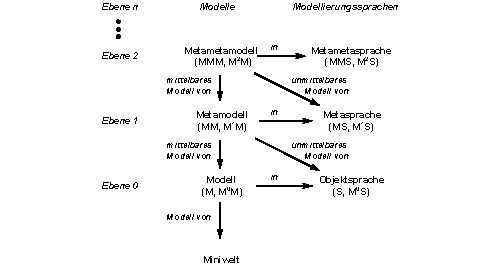
\includegraphics[width=1.45\textwidth]{figures/metamodellbegriff.svg.pdf} }
\caption{ Der sprachbasierte Metamodellbegriff. Die „Miniwelt“ entspricht dem Original. Grafik entnommen aus (Strahringer, 1998, S. 3). }\label{metamodellbegriff}
\end{figure}
 
\subsection{Metamodell des Dokumentmodells}\label{metamodell_dokument}
 
Damit das Modell formal und damit nicht verschwommen spezifiziert ist, brauchen wir ein Metamodell. Das Metamodell schafft somit auf einer abstrakteren Ebene Klarheit über das Modell.

 
Auf Abbildung \ref{docmodell} ist das eigentliche Modell visualisiert. Dieses soll vom Metamodell beschrieben werden.

 
\begin{figure}[h!]
\centering
\advance\leftskip-2.5cm
\fbox{ 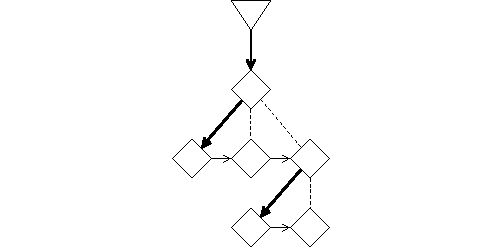
\includegraphics[width=1.45\textwidth]{figures/docmodell.svg.pdf} }
\caption{ Das hier verwendete Dokumentmodell. Das Dreieck symbolisiert die Wurzel. Die Rauten symbolisieren jeweils einen Aktor bzw. ein Dokumentelement. Die stark gezeichneten Pfeile symbolisieren das erste Kind, die gestrichelte Linie symoblisiert die zugehörigen anderen Kinder. Die schwach gezeichneten Pfeile symbolisieren die nächsten Geschwister. Dadurch wird die Hierarchie des Dokuments aufgespannt. }\label{docmodell}
\end{figure}
 
Abbildung \ref{metamodell} zeigt das Modell welches das Dokumentmodell beschreibt, also das „Metamodell“. In der Mitte liegt der Basis Aktor, dieser hält Referenzen zu seinem ersten Kind und zu seinem unmittelbaren Geschwister. Zudem hält der Basis Aktor Inststanzen aller verfügbaren Dokumentelemente, wovon jedoch immer nur eine aktiv ist. Welche Dokumentelemente verfügbar sind, wird vom Programmierer spezifiziert -- dazu muss er ein Scala Trait (entspricht einem Interface) implementieren und dem Basis Aktor bekannt machen. Man kann sagen, dass er das Metamodell an dieser Stelle (gewollt) verändert. Der Wurzel Aktor hält nochmals alle Topologieinformationen, daher kennt er alle im System vorhandenen Basis Aktoren. Jeder Basis Aktor kennt auch seine zugehörige Wurzel, welche er bei ggf. anstehenden lokalen Topologieveränderungen benachrichtigen muss.

 
\begin{figure}[h!]
\centering
\advance\leftskip-2.5cm
\fbox{ 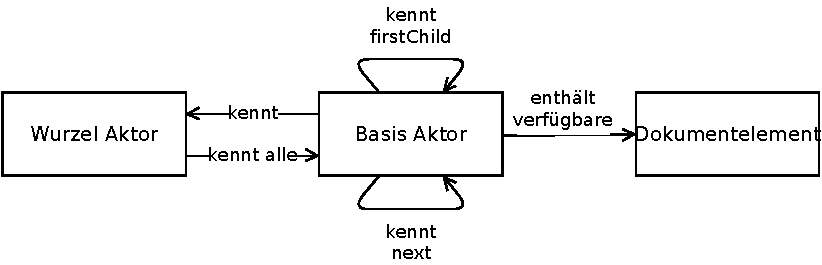
\includegraphics[width=1.45\textwidth]{figures/metamodell.svg.pdf} }
\caption{ Das Metamodell des Dokumentmodells. }\label{metamodell}
\end{figure}
 
\subsubsection{Beweis}\label{}

 
Die Besonderheit bei dem hier entstandenen System ist, dass das Modell gleichzeitig die Sprache ist, in der es modelliert wird. Dies ist möglich, da das System als Projektionseditor designed ist. Die Objektsprache in der das Modell formuliert ist, entspricht somit quasi der Projektion die direkt aus dem abstrakten Syntaxbaum entspringt. Man könnte von einem „Modell-Objektsprache-Dualismus“ sprechen -- es ist gleichzeitig Modell und Objektsprache, je nach Betrachtungspunkt.

 
Das Modell indem wiederum die Objektsprache modelliert ist, muss ein Beschreibungsmodell sein, damit dies einem Metamodell entspricht. Das hier vorgestellte Metamodell spezifiziert die Eigenschaften des Originals (dies geschieht in den einzelnen Dokumentelementen) und die prinzipielle Struktur (anschaulich gemacht durch Wurzel/Basis Aktor) des abstrakten Syntaxbaumes. Der betrachtete Gegenstandsbereich ist der abstrakte Syntaxbaum, dieser in seiner Gesamtheit, ist wiederum das Modell des Dokuments. Auf Abbildung \ref{metamodellschema} ist nochmals eine Übersichtsgrafik der Zusammenhänge von Modell und Metamodell. Somit genügt es dem Metamodellbegriff. ■

 
\begin{figure}[h!]
\centering
\advance\leftskip-2.5cm
\fbox{ 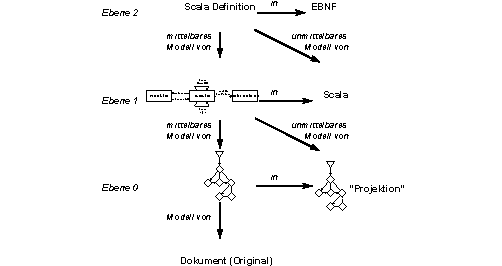
\includegraphics[width=1.45\textwidth]{figures/metamodellschema.svg.pdf} }
\caption{ Übersicht der Zusammenhänge des Dokumentmodells und Dokumentmetamodells. Grafik nach (Strahringer, 1998). Die erweiterte Backus-Naur-Form (EBNF) kann als Metametamodell dienen -- denn mit EBNF können Programmiersprachen beschrieben werden und zudem ist EBNF in der Lage sich selbst zu beschreiben. }\label{metamodellschema}
\end{figure}
 
\section{Semiotik}\label{semiotik-sec}
 
\begin{quote}
 Semeiotik [sic] ist eigentlich nichts anderes als die allgemeine Lehre von den Sprachen. Ob diese nun künstliche oder natürliche Sprachen sind, spielt keine Rolle. \citep[S.~8]{Malissa}
\end{quote}
 
Die Gesetzmäßigkeiten einer Sprache kann allgemein in vier Hauptteile gegliedert werden, vgl. \citep[S.~8]{Malissa}:

 
\begin{enumerate}[(i)]

\item
Syntax (Struktur): beschreibt die Beziehung zwischen Zeichen, Signalen, Symbolen zueinander. Hier kann man sich die Frage stellen: Was ist ein korrekter Aufbau eines Symbols? Zum Beispiel wenn man einen Satz einer natürlichen Sprache als Symbol ansieht, wird ein Satz nur durch eine bestimmten Reihung von Wörtern korrekt.


\item
Semantik (Bedeutung): „ist die Lehre von den Zeichen, Signalen, Symbolen und deren Bedeutung.“ (ebd.) Sie stellt also die Beziehung zwischen Symbol und des bezeichneten Objekts her. Hier kann man sich die Frage stellen: Was bedeutet das Symbol? Was ist die Bedeutung?


\item
Pragmatik (Funktion): stellt die Beziehung zwischen Zeichen, Signalen, Symbolen und dem Sender bzw. Empfänger dar. Hier kann man sich die Frage stellen: Was ist der Zweck des Symbols? An wen ist es, wozu gerichtet?


\item
Sigmatik (Bezeichnung): „stellt die Beziehung zwischen den Zeichen, Symbolen, Signalen usw. und dem, was sie bezeichnen her.“ (ebd.) Hier kann man sich die Frage stellen: Was bezeichnet das Symbol? Was ist das Bezeichnete?


\end{enumerate}
 
Wenn ein Zeichen, Signal, Symbol, etc. alle der oben genannten vier Aspekte aufzeigt, dann spricht man von einer Information. Im Allgemeinen sind diese vier Aspekte also die Grundlage jeder Information. In Abb. \ref{semiotik} sind die Aspekte anhand von Beispielen aus der analytischen Chemie visualisiert.

 
\begin{figure}[h!]
\centering
\advance\leftskip-2.5cm
\fbox{ 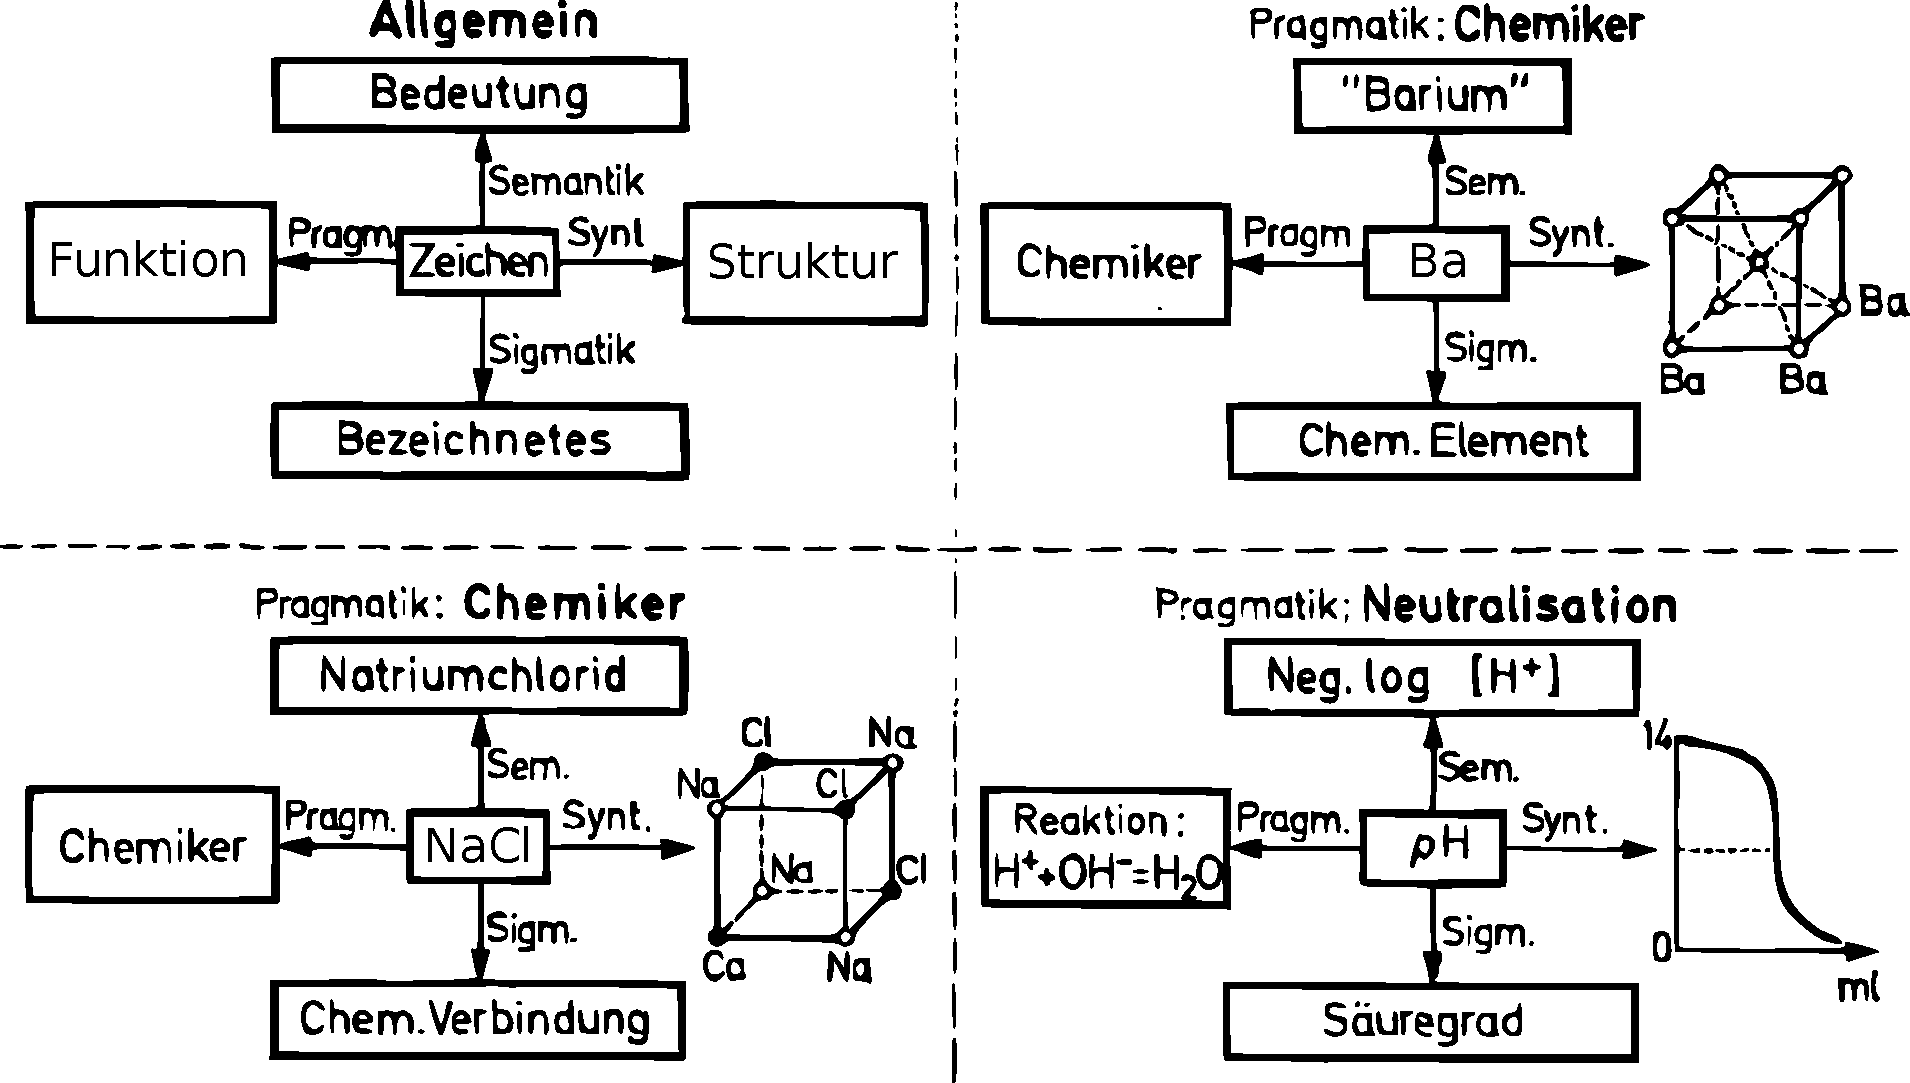
\includegraphics[width=1.45\textwidth]{figures/semiotik.svg.pdf} }
\caption{ Die vier Hauptteile der Semiotik grafisch dargestellt mit Beispielen aus der analytischen Chemie. Allgemein: Visualisierung der Semiotik eines Zeichens. Beispiel „Ba“: Ba ist ein Zeichen, dessen Bedeutung Barium ist und ein chemisches Molekül bezeichnet. Das ist zumindest dann der Fall, wenn dies von einem Chemiker gelesen wird. Strukturell ordnen sich Barium Moleküle als ein geordneter Kristall an. Analog ist es bei der chemischen Verbindung dargestellt als NaCl. Beispiel „pH“: Im Kontext einer Neutralisierungsreaktion, hat das Symbol pH die Bedeutung des der umgekehrten Logarithmusfunktion über die Konzentration der positiv geladenen Wasserstoffionen. Dies bezeichnet den Säuregrad einer Flüssigkeit. Strukturell kann es als Plot dargestellt werden. Visualisierung mit einigen Anpassungen aus (Malissa, 1971, S. 9). }\label{semiotik}
\end{figure}
 
\subsection{Anwendung auf (wiss.) Dokumente}\label{}
 
Diese vier Aspekte wirken auch implizit in jedem Text, da insbesondere wissenschaftliche Dokumente ein klassischer Informationsträger sind. In der Wissenschaft ist es üblich mit Modellen zu arbeiten. Diese Modelle sollen von anderen Wissenschaftlern möglichst leicht verstanden und benutzt werden. Für das Verstehen eines Modells ist es unerlässlich, die Bedeutungen jedes einzelnen Aspekts des Modells zu erfassen. Damit ein Leser einfach und gezielt Wissen aus dem Dokument ziehen kann, wäre es sicher nützlich, wenn diese Semantik möglichst explizit zur Verfügung stünde. Die Mechanik dazu könnte folgendermaßen aussehen: „Man fährt mit dem Mauszeiger über ein interessantes Objekt und erhält sofort weitere Informationen dazu, um mehr über die Bedeutung des Objektes zu erfahren.“

 
Wenn man die vier Konzepte allgemein auf den hier vorgestellten Prototypen überträgt, stellt man fest wie sich die Konzepte innerhalb eines Dokuments auswirken. Betrachtet wird ein einzelnes Dokumentelement:

 
\begin{itemize}

\item Zeichen: Entspricht einer Projektion des abstrakten Syntaxbaumes (z.B. ein Abschnitt-Dokumentelement gesetzt als „Kapitel 1. Einleitung“)
\item Bezeichnetes: Ist ein Dokumentelement.
\item Bedeutung: Erster gliedernder Abschnitt des Dokuments.
\item Funktion: Der Autor fungiert während des Schreibens als Sender und Empfänger.
\item Struktur: Entspricht dem abstrakten Syntaxbaum selbst bzw. dessen Metamodell.
\end{itemize}
 
Man kann argumentieren, dass hinter jedem Dokumentelement (z.B. Abschnitt, Absatz, Tabelle, ...) ein entsprechendes Domänenmodell steckt. Beispielsweise hinter einem Chemie-Dokumentelement stecke ein Moleküleditor, der ein entsprechendes Modell eines Moleküls produziert, sowie eine grafische Repräsentation (Bild eines Moleküls). Idealerweise liegt das Domänenmodell als domänenspezifische Sprache (DSL) vor. Im Bezug auf das Chemie-Dokumentelement könnte das die IUPAC-, Molfile-\footnote{~Das Molfile der Firma MDL repräsentiert chemische Strukturen. Siehe „Repräsentation chemischer Strukturen“ unter http://de.wikipedia.org/wiki/Chemoinformatik } oder SMILES-Molekülnotation sein. Das würde bedeuten, dass der hier vorgestellte Syntaxbegriff auch gleichzeitig das Domänenmodell vertritt.

 
Das heißt, dass bei der Erstellung eines Dokuments Dokumentelemente vom Autor entworfen werden können, welche Modelle der jeweiligen Wissenschaft enthalten können. Das ermöglicht dem Autor deutlich strukturierter, formaler und konsistenter an die Dokumentation seins Projektes heranzugehen. Zudem werden dem Leser dadurch explizite semantische Informationen bereitgestellt, welche direkt vom dahinterstehenden Modell stammen. Der Leser kann ggf. das Modell seines Kollegen in eigenen Dokumenten wiederverwenden. Vorteil hierbei wäre, dass weniger Fehler entstehen, da direkt auf die Gedanken (welche in das Modell gegossen wurden) des Original-Autors zurückgegriffen werden kann.

 
Üblicherweise gibt es unter Dokumentelementen Verweise. Zum Beispiel ein Absatz-Dokumentelement möchte auf die Molekülmasse des Chemie-Dokumentelements verweisen. Dann sieht die Semiotik folgendermaßen aus:

 
\begin{itemize}

\item Zeichen: „Die Molekülmasse ist 144 g/mol.“ (So angezeigt durch den Absatz)
\item Bezeichnetes: Chemie(molekül)-Dokumentelement. (Welches das Modell des Moleküls enthält)
\item Bedeutung: Masse von Koffein in Gramm pro Mol. (Interessantes Objekt wäre „144 g/mol“)
\item Funktion: Verweis
\item Struktur: „{ koffein.masse }“ (hieraus folgt „144 g/mol“)
\end{itemize}
 
Mechanik: Der Programmierausdruck „koffein.masse“ („koffein“ wäre der Name des Chemie-Dokumentelements und „masse“ eine bereitgestellte Methode des Chemie-Dokumentelement-Objektes) liefert ein semantisches Objekt, z.B. in Form eines Scala-Objekts des Typs Moleculemass. Moleculemass könnte mit den Properties mass, name, unit ausgestattet sein, um mehr Informationen über seine Bedeutung(en) bereitstellen zu können. Zudem könnte es noch an eine SI-Einheiten-Onologie angekoppelt sein, um die semantischen Informationen mit dem Semantic Web zu teilen. Wenn der Leser mit seinem Mauszeiger über „144 g/mol“ fährt, kann diese Information aus dem Moleculemass-Objekt geholt werden und in Form einer farbigen Annotation angezeigt werden.

 
\section{Taxonomie wissenschaftlicher Publikationen}\label{taxonomie-sec}
 
Über die Jahrhunderte in denen wissenschaftliche Texte verfasst wurden, haben sich gewisse Konventionen und Vorgehensmodelle, wie ein Dokument von seinem inneren Aufbau her beschaffen sein soll, herauskristallisiert. Diese Konventionen haben sich sogar über nationale Grenzen hinweg sehr ähnlich entwickelt, was es der Wissenschaftsgemeinde leichter macht, ihr intellektuelles Vermächtnis zu teilen.

 
In Recherchen ist aufgefallen, dass es schon (wenn auch wenige) Versuche gegeben hat, eine möglichst allgemeingültige Systematik (z.T. formal) des inneren Dokumentenaufbaus herauszudestillieren. Jedoch sind diese Konzepte bisher kaum verbreitet, insbesondere bei der direkten Erstellung von (wiss.) Texten durch den Autor. Heutige Textverarbeitungen unterstützen kaum explizite Semantik über das Domänenwissen, mit dem sie gerade arbeiten -- dies fördert Fehler und Inkonsistenzen im Dokument.

 
Die DIN-Normen \citep{DIN1421}, \citep{DIN1422-1}, \citep{DIN1422-3} und \citep{DIN1422-4} geben Empfehlungen, wie Texte gegliedert und benummert werden sollen bzw. wie im allgemeinen Manuskripte oder Forschungsberichte gestaltet werden sollen. Dies sind keine formalen Vorgaben, sondern vielmehr eine Zusammenfassung der hiesigen guten fachlichen Praxis in Wissenschaft, Technik, Wirtschaft und Verwaltung. Anders hingegen geht \citep{NISO} vor, hier wird formal mittels XML Schemas eine allgemein gültige Menge an XML-Tags für den Aufbau von Fachzeitschriftenartikeln zusammengestellt. Jedoch haben diese auch für anderen Publikationen ihre Gültigkeit, wie z.B. Briefe, Leitartikel oder Buchkritiken. \citep{Peroni} stellt eine Ontologie (in OWL 2) über einzelnen Komponenten, die in einem Dokument vorkommen können, zur Verfügung. Hier werden die Beziehungen die die Komponenten untereinander pflegen sichtbar gemacht. Es wird dabei zwischen strukturierenden (z.B. Abschnitt, Absatz) und rhetorischen Komponenten (z.B. Einleitung, Abbildung, Anhang) unterschieden.

 
Hier soll versucht werden die Erkenntnisse der o.g. Quellen zu generalisieren, in der Hoffnung die Basis für ein formaleres bzw. präskriptiveres Textverarbeitungssystem zu schaffen.

 
\subsection{Dokumentelemente}\label{dokumentelemente}
 
Dokumentelemente bilden das Grundgerüst eines jeden Dokuments. Hier wird versucht den Begriff genauer zu fassen und zu definieren. Es ergeben sich drei abstrakte Ausprägungen der Dokumentelemente:

 
\begin{itemize}

\item Struktur Elemente: repräsentieren Komponenten, die textuellen bzw. grafischen Inhalt des Dokuments beinhalten. Sie tragen maßgeblich zum gedanklichen Gebäude des Dokuments bei.
\item Container Elemente: beinhalten andere Dokumentelemente (als Kinder), und haben daher für gewöhnlich keine Repräsentation die aktiv zum eigentlichen intellektuellen Inhalt des Dokuments beiträgt. Sie gruppieren also Elemente zu größeren Dokument-Bestandteilen; dies gibt Vorteile bei der Verarbeitung und Semantik des Dokuments. Beispielsweise werden Dokumente oft in Titelei und Hauptteil unterteilt, wobei die Titelei gerne römisch nummeriert wird und der Hauptteil arabisch. Hat man hier eine explizite Hierarchievorgabe zur Hand, erleichtert das die Verarbeitung; wie im Beispiel die gewollten Nummerierungskonventionen durchzusetzen.
\item Metadaten Elemente: sind Elemente die andere Elemente beschreiben bzw. allgemein gesprochen enthalten sie Daten über Daten. Beispielsweise ein Literatureintrag beschreibt lediglich einen Original-Artikel; oder eine Fußnote enthält eine Anmerkung über ein anderes Dokumentelement (die Fußnote verändert den Inhalt den das Dokument transportieren will an sich nicht, aber sie macht ihn verständlicher).
\end{itemize}
 
Die Dokumentelemente können zudem auch noch Attribute oder Properties enthalten. Diese enthalten Fakten über das betreffende Element, z.B. ob es sich bei einer Liste um eine geordnete Liste oder ungeordnete Liste handelt. Im Falle des hier vorgestellten Prototypen, kann man argumentieren, dass in den Attributen auch das jeweils vorliegende Domänenmodell des Dokumentelements abgelegt wird.

 
In DoCO wird ein Unterschied zwischen strukturierenden (z.B. Abschnitt, Absatz) und rhetorischen Komponenten (z.B. Einleitung, Diskussion, Abbildung) unterschieden. Hier wird jedoch nur das Struktur Element benötigt, da die rhetorische Bedeutung über die Attribute des Elements hinzugefügt werden kann. Allgemein gesprochen gehört die rhetorische Bedeutung zur Semantik des Elements. Die Semantik des Elements wird wiederum maßgeblich über das Domänenmodell gewonnen und dieses ist wiederum in den Attributen ansässig. Daher muss kein Unterschied zwischen strukturierenden und rhetorischen Komponenten gemacht werden.

 
\subsubsection{Bedeutung für das Dokumentmodell}\label{}

 
Im Dokumentmodell, also dem abstrakten Syntaxbaum entsprechen die Struktur Elemente den Blättern und die Container Elemente entsprechen den inneren Knoten. Metadaten Elemente kommen entweder wie Struktur Elemente vor oder werden in ein extra „Metadokument“ ausgelagert, falls die Metadaten Elemente nur einzelne Attribute bereitstellen sollen und nicht in Gänze angezeigt werden.

 
\subsubsection{Verweisungen}\label{}

 
\citep{Peroni} und \citep{NISO} modellieren mehr Dokumentelemente als in der vorgestellten Taxonomie (s. Abschnitt \ref{taxonomiesec}). Das liegt zum einen daran, dass hier viele dieser „Elemente“ in dem hier vorgestellten Modell als Attribute abgelegt werden. Hier treten nur die Komponenten explizit als Dokumentelement auf, bei denen es Sinn macht auch als ein Knoten des abstrakten Syntaxbaumes abgebildet zu werden. Zum anderen werden in den Modellen von (ebd.) Verweisungen, die sich innerhalb des Dokuments abspielen (z.B. auf Kapitel oder Abbildungen), auch explizit als Dokumentelement modelliert. Dies macht aber in dem hier vorgestellten Dokumentmodell wenig Sinn.

 
Denn hier treten Verweisungen nicht in Form von Knoten auf, sondern sie entsprechen den Kanten des Dokumentengraphs. Wenn ein Knoten (also Dokumentelement) eine Information von einem anderen Knoten erhalten will, werden Nachrichten mit den Informationen ausgetauscht. Durch diesen Mechanismus werden die Verweisungen im Dokument schlussendlich aufgelöst. Wir haben also ein ganz klares Modell: Inhalte in die Blätter, Hierarchie in die inneren Knoten, Semantik und Modelle in die Attribute und Verweisungen fließen über die Kanten, also in der Implementierung des Prototypen als Nachrichten-Kommunikation.

 
\subsection{Taxonomie}\label{taxonomiesec}
 
In der Tabelle auf Abb. \ref{taxonomie} sind nochmals alle drei Ausprägungen der Dokumentelemente (s. Abschnitt \ref{dokumentelemente}) übersichtlich dargestellt. Sie sind von abstrakt zu konkreter werdend geordnet. In der vorletzten Spalte sind die eigentlichen Kernelemente aufgezeigt, welche auch so im Dokument vorkommen können. In der letzten Spalte sind mögliche Attribute, Properties bzw. Methoden aufgelistet, die dem Element zusätzliche (semantische) Informationen hinzufügen.

 
Mit den in der Tabelle (Abb. \ref{taxonomie}) aufgelisteten Dokumentelementen kann man ein typisches, aber sehr allgemein gehaltenes, wissenschaftliches Dokument aufbauen. Die Gesamtheit der hier vorliegenden Dokumentelemente beschreibt somit eine ganz bestimmte Dokumentklasse, welche als allgemeiner „wissenschaftlicher Bericht“ oder „Report“ bezeichnet werden kann. Aber es gibt auch noch beliebige andere Klassen (z.B. Patente, Normen, Softwaredokumentation, etc.), die möglicherweise einen (leicht) anderen Aufbau haben und somit ggf. andere Dokuementelemente benötigen. Neu definierte Dokumentelemente (z.B. für eine andere Dokumentklasse) sollten sich leicht in diese Taxonomie eingliedern lassen. Damit liegen sie nicht mehr als implizite Aufbauvorschrift (gemeint ist so etwas wie ein Corporate Design) vor, sondern sind explizit, für die Nutzung in einem Textverarbeitungssystem welches die Taxonomie umsetzt, formalisiert.

 
\begin{figure}[h!]
\centering
\advance\leftskip-2.5cm
\fbox{ 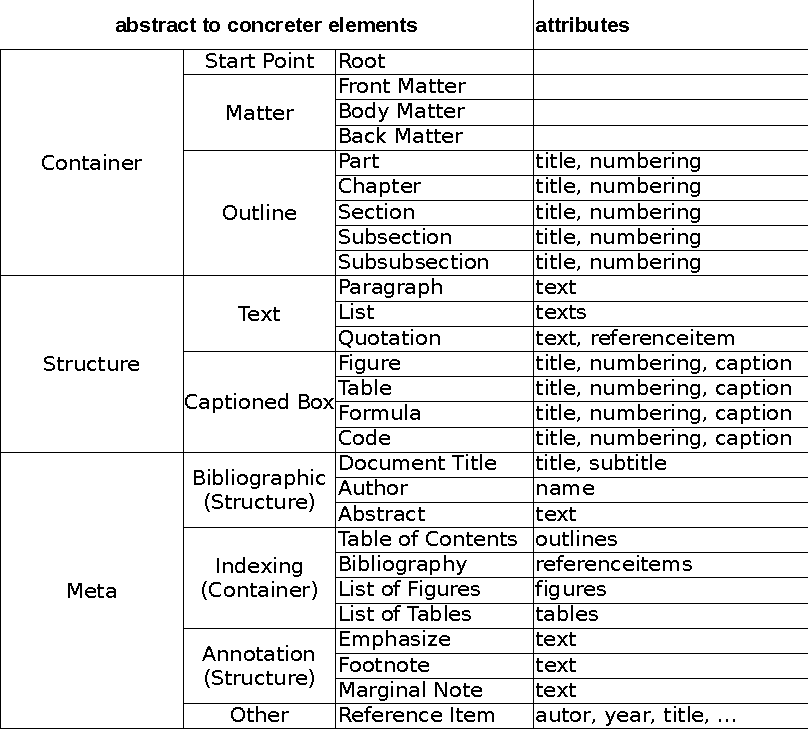
\includegraphics[width=1.45\textwidth]{figures/taxonomie.svg.pdf} }
\caption{ Taxonomie des inneren Aufbaus von wissenschaftlichen Dokumenten. Sortiert von abstrakt zu konkret. Anmerkung: Die Tabelle ist in englischer Sprache gehalten, da die Namen den Implementierungsnamen im Prototyp entsprechen. }\label{taxonomie}
\end{figure}
 
\subsection{Dokumentstruktur Matrix}\label{}
 
Damit das Textverarbeitungssystem beim Erstellen eines formal korrekten Dokuments helfen kann, wird ein Regelwerk benötigt welches vorschreibt „welches Element nach wem erlaubt ist“ (erlaube Geschwister-Beziehungen) und „wo darf welches Element vorkommen“ (erlaube Eltern-Kind-Beziehungen).

 
Durch diese Formalisierung kann der Autor wie auf Schienen durch den Aufbau geführt werden. Er muss sich also nicht mehr selbst darum kümmern die impliziten Vorgaben der Dokumentklasse durchzusetzen. Das heißt, er macht weniger Fehler beim Aufbau des Dokuments, da das System assistierend zur Seite steht, um die gewählte Dokumentklasse ihrem Regelwerk konform zu halten und er sich stärker auf die Erstellung des Inhalt konzentrieren kann. Zudem liefert jedes Dokumentelement ein Set an Attributen mit, was es ermöglicht mehr explizite Semantik in das Dokument zu bringen und das Dokument insgesamt konsistenter zu halten.

 
\subsubsection{Erlaube Verschachtelungen}\label{}

 
Auf Abbildung \ref{matrixkind} sind die erlaubten Eltern-Kind-Beziehungen der vorliegenden Dokumentklasse definiert. Die hier dargestellte Matrix ist eine Vereinfachung, also nur eine Auswahl an Dokumentelementen, der Taxonomie aus Tabelle auf Abb. \ref{taxonomie}. Diese Matrix definiert die erlaube Schachtelung der vorliegenden Dokumentklasse.

 
\begin{figure}[h!]
\centering
\advance\leftskip-2.5cm
\fbox{ 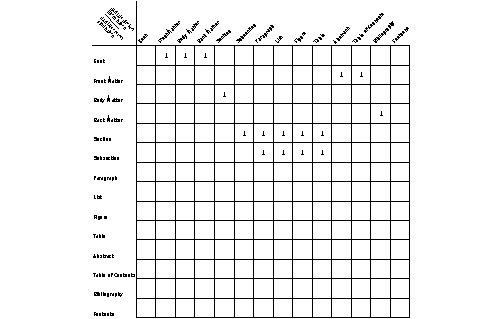
\includegraphics[width=1.45\textwidth]{figures/matrixkind.svg.pdf} }
\caption{ Stellt die erlaubten Eltern-Kind-Beziehungen zwischen den Dokumentelementen dar. Hier wird also definiert mit welchen Elementen die Hierarchie des Dokuments aufgespannt werden darf. Gelesen wird es z.B. von links nach oben: Body Matter darf als Kind Section haben. Oder von oben nach rechts: Section darf als Eltern Body Matter haben. Es fällt auf, dass die Matrix unterhalb der Determinanten leer ist. Das liegt daran, dass Containerelemente keine Strukturelemente als Eltern haben dürfen. }\label{matrixkind}
\end{figure}
 
\subsubsection{Erlaube Abfolgen}\label{}

 
Auf Abbildung \ref{matrixgeschwister} sind die erlauben Nachfolger-Vorgänger-Bezeihungen der hier beispielhaft vorliegenden Dokumentklasse als Matrix dargestellt. Hier wird also die Frage geklärt, welches Dokumentelemente aneinander gereiht werden dürfen, um ein wohlgeformtes Dokument der vorliegenden Dokumentklasse zu bilden.

 
\begin{figure}[h!]
\centering
\advance\leftskip-2.5cm
\fbox{ 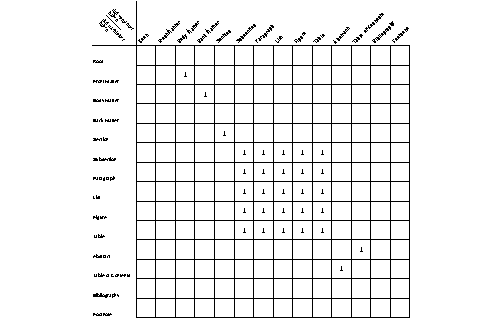
\includegraphics[width=1.45\textwidth]{figures/matrixgeschwister.svg.pdf} }
\caption{ Stellt die erlaubten Geschwister-Beziehungen (Nachfolger/Vorgänger) zwischen den Dokumentelementen dar. Hier wird also definiert welche Elementen aneinandergereiht werden dürfen. Es fällt auf, dass Strukturelemente eine Gruppe bilden, da sie nur als Blätter vorkommen. }\label{matrixgeschwister}
\end{figure}
 
\subsection{Deutung}\label{}
 
Wenn man also ein Set an Dokumentelementen definiert und in die Taxonomie eingegliedert hat, zudem noch die erlaubten Beziehungen zwischen den Dokumentelementen in Matrixform definiert hat, dann erhält man eine präzise definierte Dokumentklasse. Nützlich ist das nicht nur um dem Autor „Schienen“ für die Dokumenterstellung bereitzustellen, sondern auch für Klassifikationsaufgaben. Beispiel: Im Zuge von Information Retrieval hat man verschiedene mit OCR aufbereitete PDFs, welche man gerne einer Dokumentklasse zuordnen möchte, um sie wieder in ein „sauberes“ oder aktuelles Template zu überführen. Wenn nun ein Klassifikator die aufbereiteten PDFs in ihre Dokumentelemente zerlegt, kann über die Gesamtheit der im PDF gefunden Dokumentelemente und deren Anordnung bzw. Verschachtelung, dank der aufgestellten Taxonomien bzw. Matrizen, auf die Dokumentklasse (z.B. EU-Patent, US-Patent, DIN-Norm, etc.) zurückgeschlossen werden.

 
\chapter{Anwendungsfälle}\label{}
 
\section{Erstellung wissenschaftlicher Dokumente}\label{wiss-dok-abschnitt}
 
In erster Linie soll das System Autoren bei der Erstellung hochwertiger wissenschaftlicher Berichte helfen.

 
Diese Masterarbeit selbst wurde mit dem in ihr beschriebenen Prototypen erstellt. Dies veranschaulicht die Tragfähigkeit der Konzepte, bzw. die Stabilität der momentanen Prototypen-Implementierung.

 
Damit das Dokument später auch der Hochschule bzw. Fakultät vorgelegt werden kann, muss es auch noch in einem printfähigen Format (insb. mit Paginierung) vorliegen.  Da zur Zeit noch keine Paginierung der Web-Ansicht erfolgt, muss auch noch auf ein anderes Werkzeug zurückgegriffen werden, um ein printfähiges Format zu erhalten. Da das System, dank des abstrakten Syntaxbaumes fähig ist, das Dokument in verschiedene Ansichten zu präsentieren, kann auch LaTeX-Code generiert werden.  Nähere Erklärungen zu solchen Transformationen in Abschnitt \ref{transformation}. Das heißt die Print-Version der Masterarbeit kann zudem noch via LaTeX erzeugt werden. In Zukunft sollte es jedoch kein Problem darstellen eine Print-Paginierung in die Web-Ansicht zu integrieren, dazu kann der Layouter „scaltex.js“, welcher in der Bachelorarbeit \citep{Hodapp} entstanden ist, eingesetzt werden.

 
Um einen wissenschaftlichen Text, wie eine Masterarbeit, verfassen zu können, müssen einige (Basis) Dokumentelemente vom Prototyp bereitgestellt werden, zudem müssen Verweise unter den Dokumentelementen möglich sein. Beispielsweise (mit den Implementierungsnamen): Chapter, Section, SubSection, SubSubSection und Figure mit automatischer Benummerung; Paragraph, List, ArabicList, RomanList, Quotation, Footnote; FrontMatter, BodyMatter, BackMatter.

 
\subsection{Szenario: Chemie}\label{chemie-szenario}
 
Für Demonstrationszwecke wurde auch ein Chemie-Dokumentelement erstellt, welches einen Moleküleditor anbietet. Damit wäre der Autor komfortabel in der Lage in seinem Dokument direkt chemische Moleküle zu zeichnen und darauf zu verweisen. Der Moleküleditor produziert Molfiles\footnote{~Das Molfile der Firma MDL repräsentiert chemische Strukturen. Siehe „Repräsentation chemischer Strukturen“ unter http://de.wikipedia.org/wiki/Chemoinformatik } als Ausgabe- bzw. Austauschformat, dieses Molfile ist also ein (persistentes) Modell für ein Molekül. Das Chemie-Dokumentelement könnte noch an eine Chemie-Bibliothek, die Molfiles verarbeiten kann, angebunden werden. Eine solche Programmbibliothek kann weitere Informationen zu den verwiesenen Molekülen bereitstellen, und damit einen erheblichen Beitrag zur expliziten Semantik und Konsistenz des Dokument beitragen.

 
In Abbildung \ref{Aspirin} ist ein durch das Chemie-Dokumentelement generiertes Molekül abgebildet. Wenn man darauf klickt, wird der Domäneneditor Ketcher geöffnet (s. Abb. \ref{chemieeditieren}). Ketcher\footnote{~Webseite des Ketcher Projekts: http://ggasoftware.com/opensource/ketcher} ist ein in Javascript geschriebener Moleküleditor für den Webbrowser. Das Chemie-Dokumentelement, ist lediglich ein Wrapper\footnote{~„Wrapper (Software), ein Programm, das als Schnittstelle zwischen zwei anderen Programmen dient“. Aus Wikipedia http://de.wikipedia.org/wiki/Wrapper} für diesen Moleküleditor und verwendet die Ketcher-API, um ein SVG-Bild aus dem Molekül für die Visualisierung zu generieren.

 
\begin{figure}[h!]
\centering
\advance\leftskip-2.5cm
\fbox{ 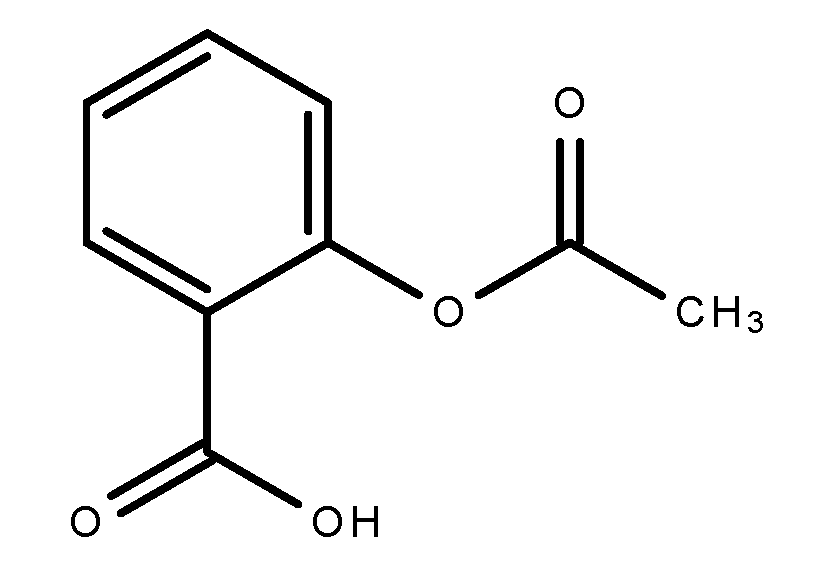
\includegraphics[width=1.45\textwidth]{figures/Aspirin.svg.pdf} }
\caption{ Generiertes Molekül Aspirin. }\label{Aspirin}
\end{figure}
 
\begin{figure}[h!]
\centering
\advance\leftskip-2.5cm
\fbox{ 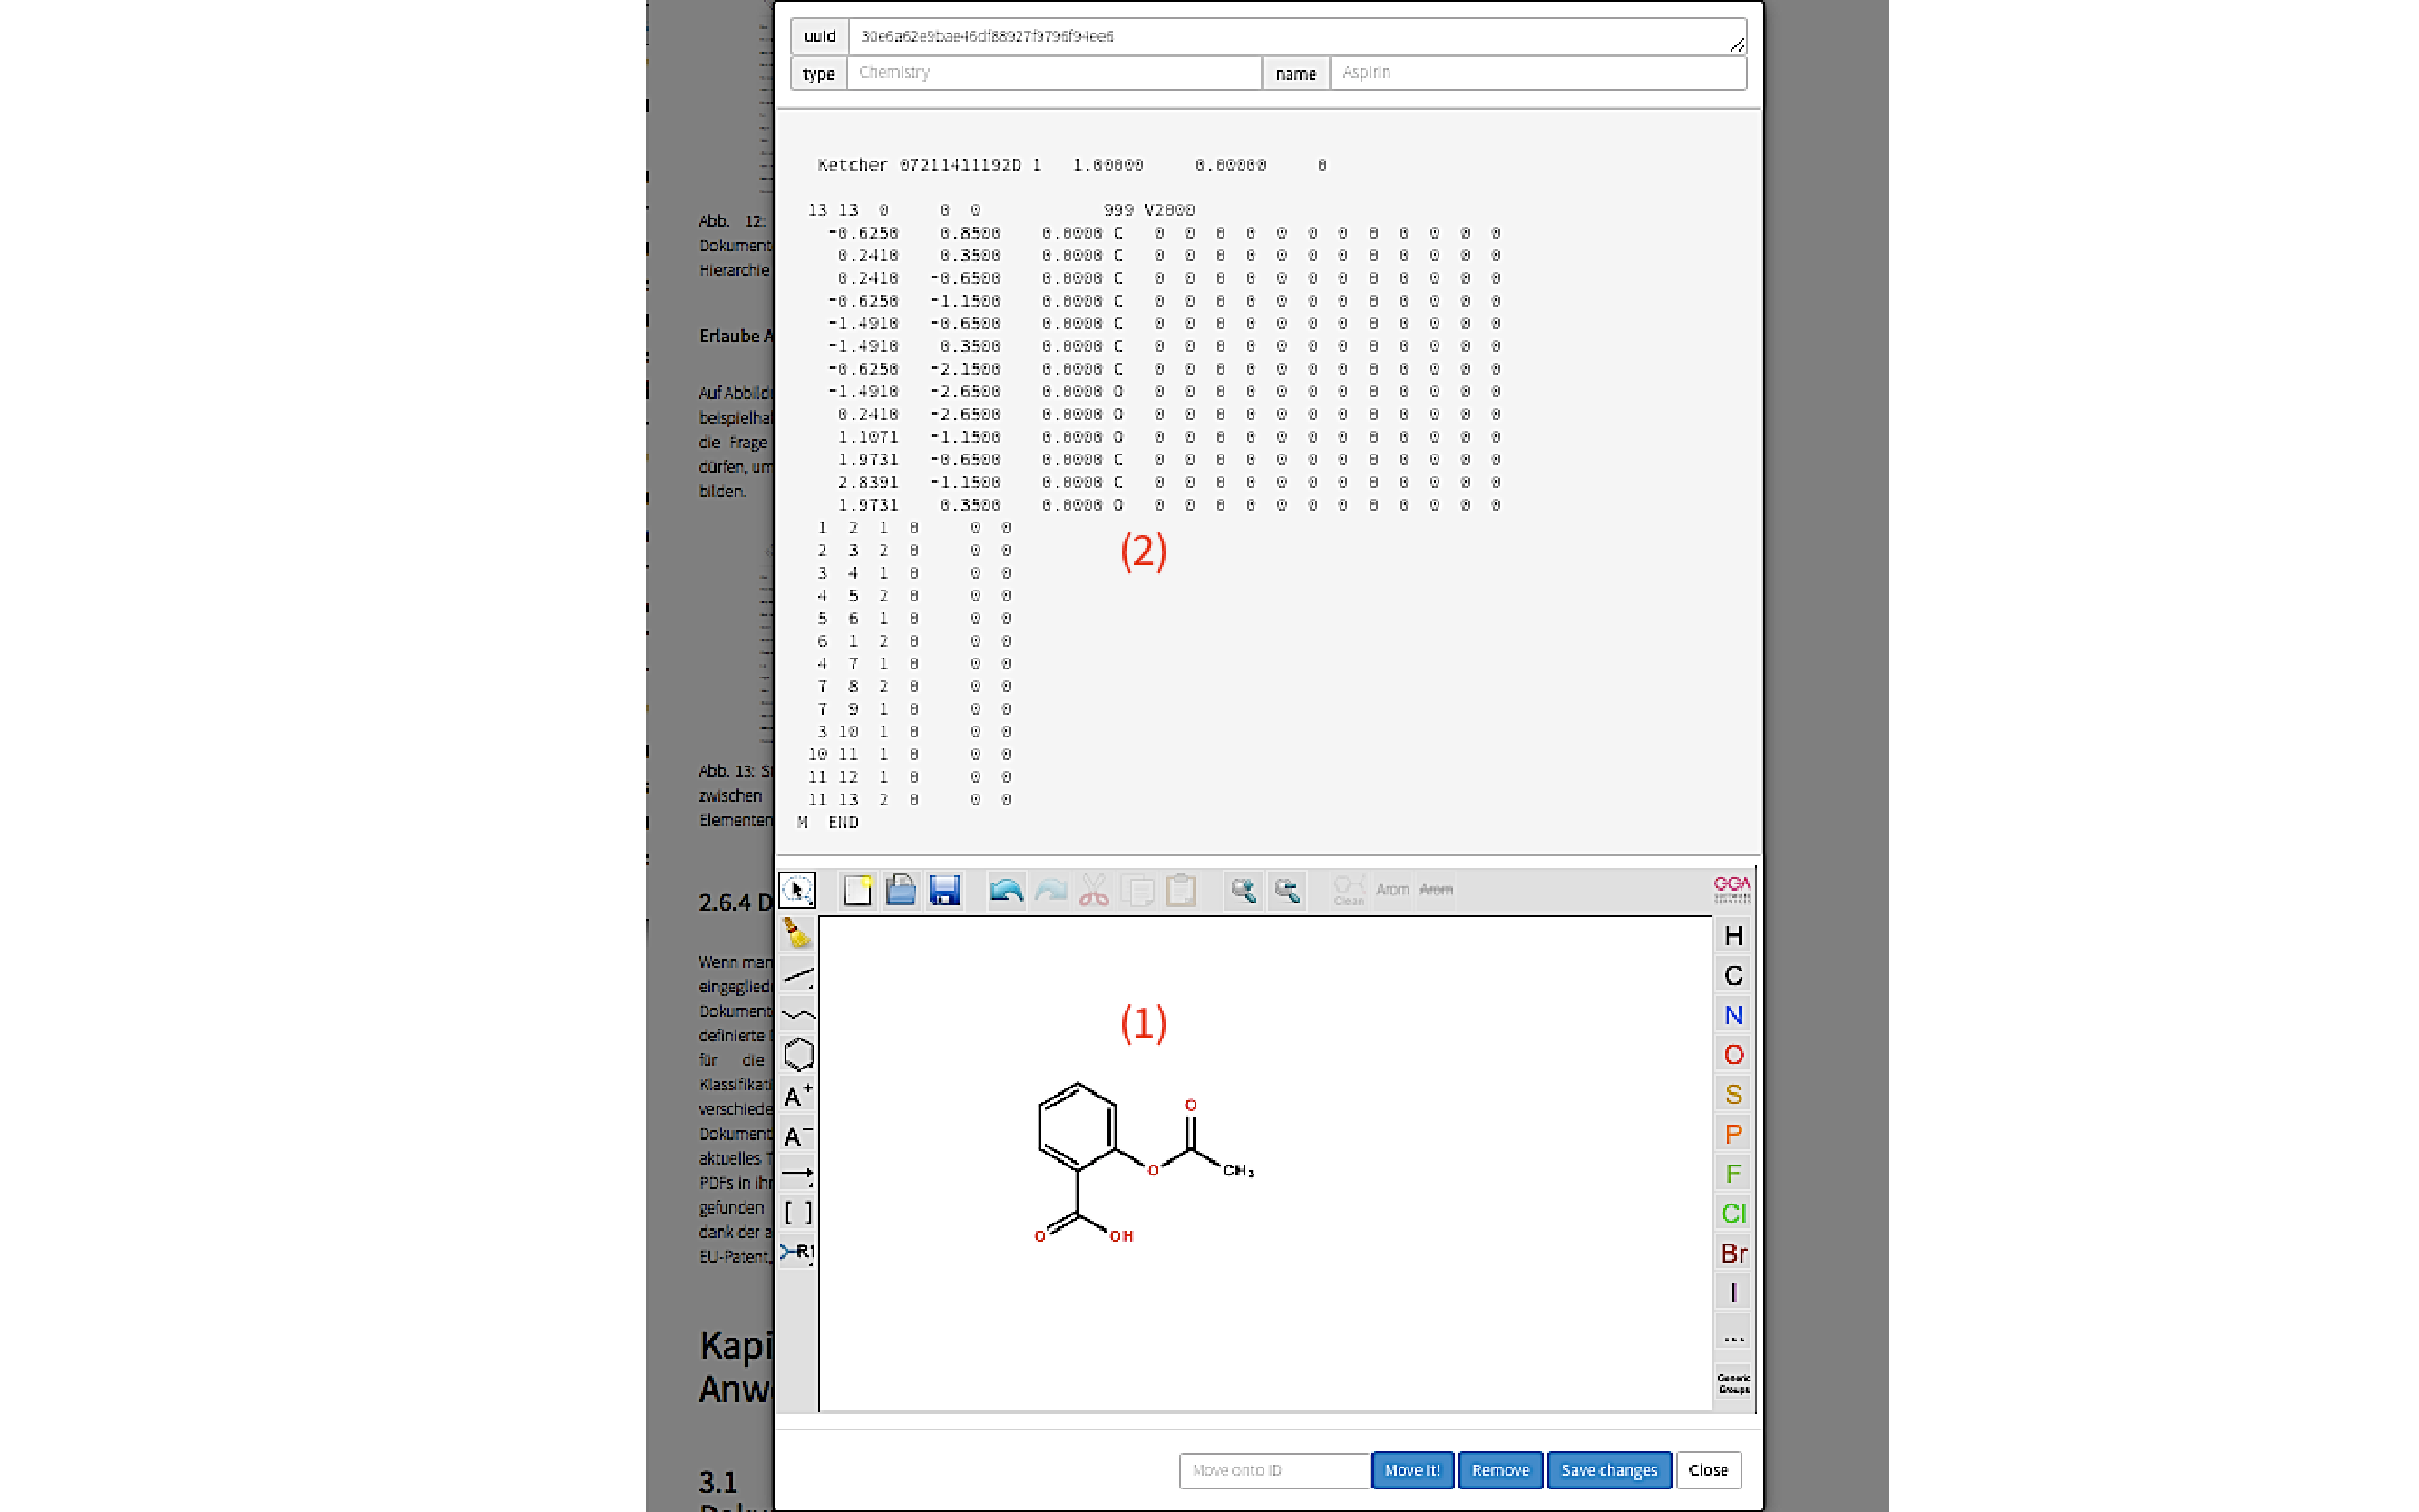
\includegraphics[width=1.45\textwidth]{figures/chemieeditieren.png.pdf} }
\caption{ Bildschirmaufnahme der Editier-Ansicht des Chemie-Dokumentelements. Es ist der Domäneneditor „Ketcher“ (1) zu sehen, der gerade das Aspirin Molekül anzeigt und zum editieren einlädt. Zudem wird das Modell (2) des Aspirin Moleküls im Molfile-Format angezeigt. }\label{chemieeditieren}
\end{figure}
 
\section{UIMA CAS Editor}\label{uima-cas-kapitel}
 
Apache UIMA\footnote{~Webseite des Apache UIMA (Unstructured Information Management Architecture) Projekts: http://uima.apache.org } ist ein Softwaresystem, mit dessen Hilfe neues, für den Benutzer relevantes, Wissen aus großen unstrukturierten Datenmengen gewonnen werden kann.

 
Ein einfacher Text kann um Anmerkungen, sogenannte Annotationen, angereichert werden. Diese Annotationen sind dafür zuständig, einzelne Entitäten des Texts zu identifizieren, wie z.B. Personen, Orte, Organisationen etc. oder Relationen wie „arbeitet für“.

 
CAS (Common Analysis System) Objekte bieten Zugriff auf das Typsystem, Indexe, Iteratoren und Filter von UIMA. Insbesondere ist es möglich, Annotationen mit dem CAS Objekt zu erstellen. Das heißt: In einem CAS Objekt kann ein Dokument mit Annotationen gespeichert werden. Ein solches CAS Objekt kann in das XML Metadata Interchange (XMI) Format serialisiert werden, wodurch es möglich ist, annotierte Dokumente zu persistieren und auszutauschen.

 
Mit einem CAS\footnote{~UIMA CAS Objekt Dokumentation: http://uima.apache.org/downloads/releaseDocs/2.3.0-incubating/docs/api/org/apache/uima/cas/CAS.html} Editor würde ein Autor also gerne im betrachteten Dokument mit Annotationen arbeiten:

 
\begin{enumerate}

\item Annotationen anzeigen,
\item Annotation bearbeiten und
\item Annotationen hinzufügen.
\end{enumerate}
 
\subsection{Konzeptuelle Umsetzung}\label{}
 
Für jeden Annotations-Typ (z.B. Person, Ort, etc.) müsste ein entsprechendes Dokumentelement angelegt werden, d.h. das Metamodell des Dokuments muss entsprechend erweitert werden. Wenn das Metamodell um die gewünschte Menge an Annotations-Typen erweitert ist, kann der Prototyp automatisch mit den neuen Dokumentelementen bzw. Annotationen umgehen. Da jedes Dokumentelement das Modell seiner Domäne vertritt, können hier auch zusätzliche (semantische) Informationen, die für die jeweilige Annotation wichtig sind, abgelegt werden.

 
\begin{quote}
 Annotation bedeutet „Anmerkung“, „Beifügung“, „Hinzufügung“. In diesem Sinn haben Annotationen bei Stichworten, Begriffsklärungen oder ausführlichen Texten den Charakter der Erklärung beziehungsweise Ergänzung. Annotationen halten Dinge fest, die zwar nicht als wesentlich für das Hauptstichwort oder den Haupttext erachtet werden, aber wichtige Zusatzinformationen darstellen. Sie sind es immerhin wert, ausdrücklich festgehalten zu werden, und auf diese Weise erhalten die bezeichneten Inhalte einen Platz in der Ordnung des Ganzen, ohne die Struktur zu stören oder die Sinnlinie der Aussage zu unterbrechen. \citep{WikiAnnotation}
\end{quote}
 
Das heißt, Annotationen sind nicht zwingender Bestandteil des eigentlichen Dokuments, welches den intellektuellen Inhalt liefert. Sie sind eher Stützen welche das Dokument leichter verständlich machen. Daher können sie den Metadaten Dokumentelementen zugeordnet werden.

 
Für diesen Zweck wurde im Prototyp ein Metadokument implementiert, dieses enthält Zusätze oder Aussagen, die vom eigentlichen Dokument separiert sein sollen. Das Metadokument bedient sich der gleichen Infrastruktur, die auch das Hauptdokument nutzt. Sie haben einen  gemeinsamen Dokumentelement-Pool und können daher gegenseitig auf die vorkommenden Dokumentelemente zugreifen, z.B. via Verweis. Schöner Nebeneffekt: Die Annotationen können im Metadokument übersichtlich angeordnet und dort ggf. dokumentiert werden.

 
Annotationen werden durch ein „mouse over“ im Browser farbig hervorgehoben (s. Abb. \ref{annotation}). Im Metadokument können neue Annotationen hinzugefügt werden und via Verweis in ein beliebiges Dokumentelement gebracht werden. Im Metadokument können sie auch bearbeitet werden. Für Demonstrationszwecke wurde das Dokumentelement „Annotation“ implementiert. Als Beispieldokumente dienen Patentschriften, die durch das vom Fraunhofer SCAI geleitete Projekt \emph{UIMA-HPC}\footnote{~Webseite des UIMA-HPC Projekts: http://uima-hpc.org} digitalisiert, durchsuchbar und annotiert wurden. Das SCAI.BIO abteilungsinterne Werkzeug „The Interfacer“ kann CAS Objekte (in denen die Patentschriften u.a. vorliegen) in Datenstrukturen des Prototypen übersetzen und somit für den Prototypen mühelos nutzbar machen.

 
\begin{figure}[h!]
\centering
\advance\leftskip-2.5cm
\fbox{ 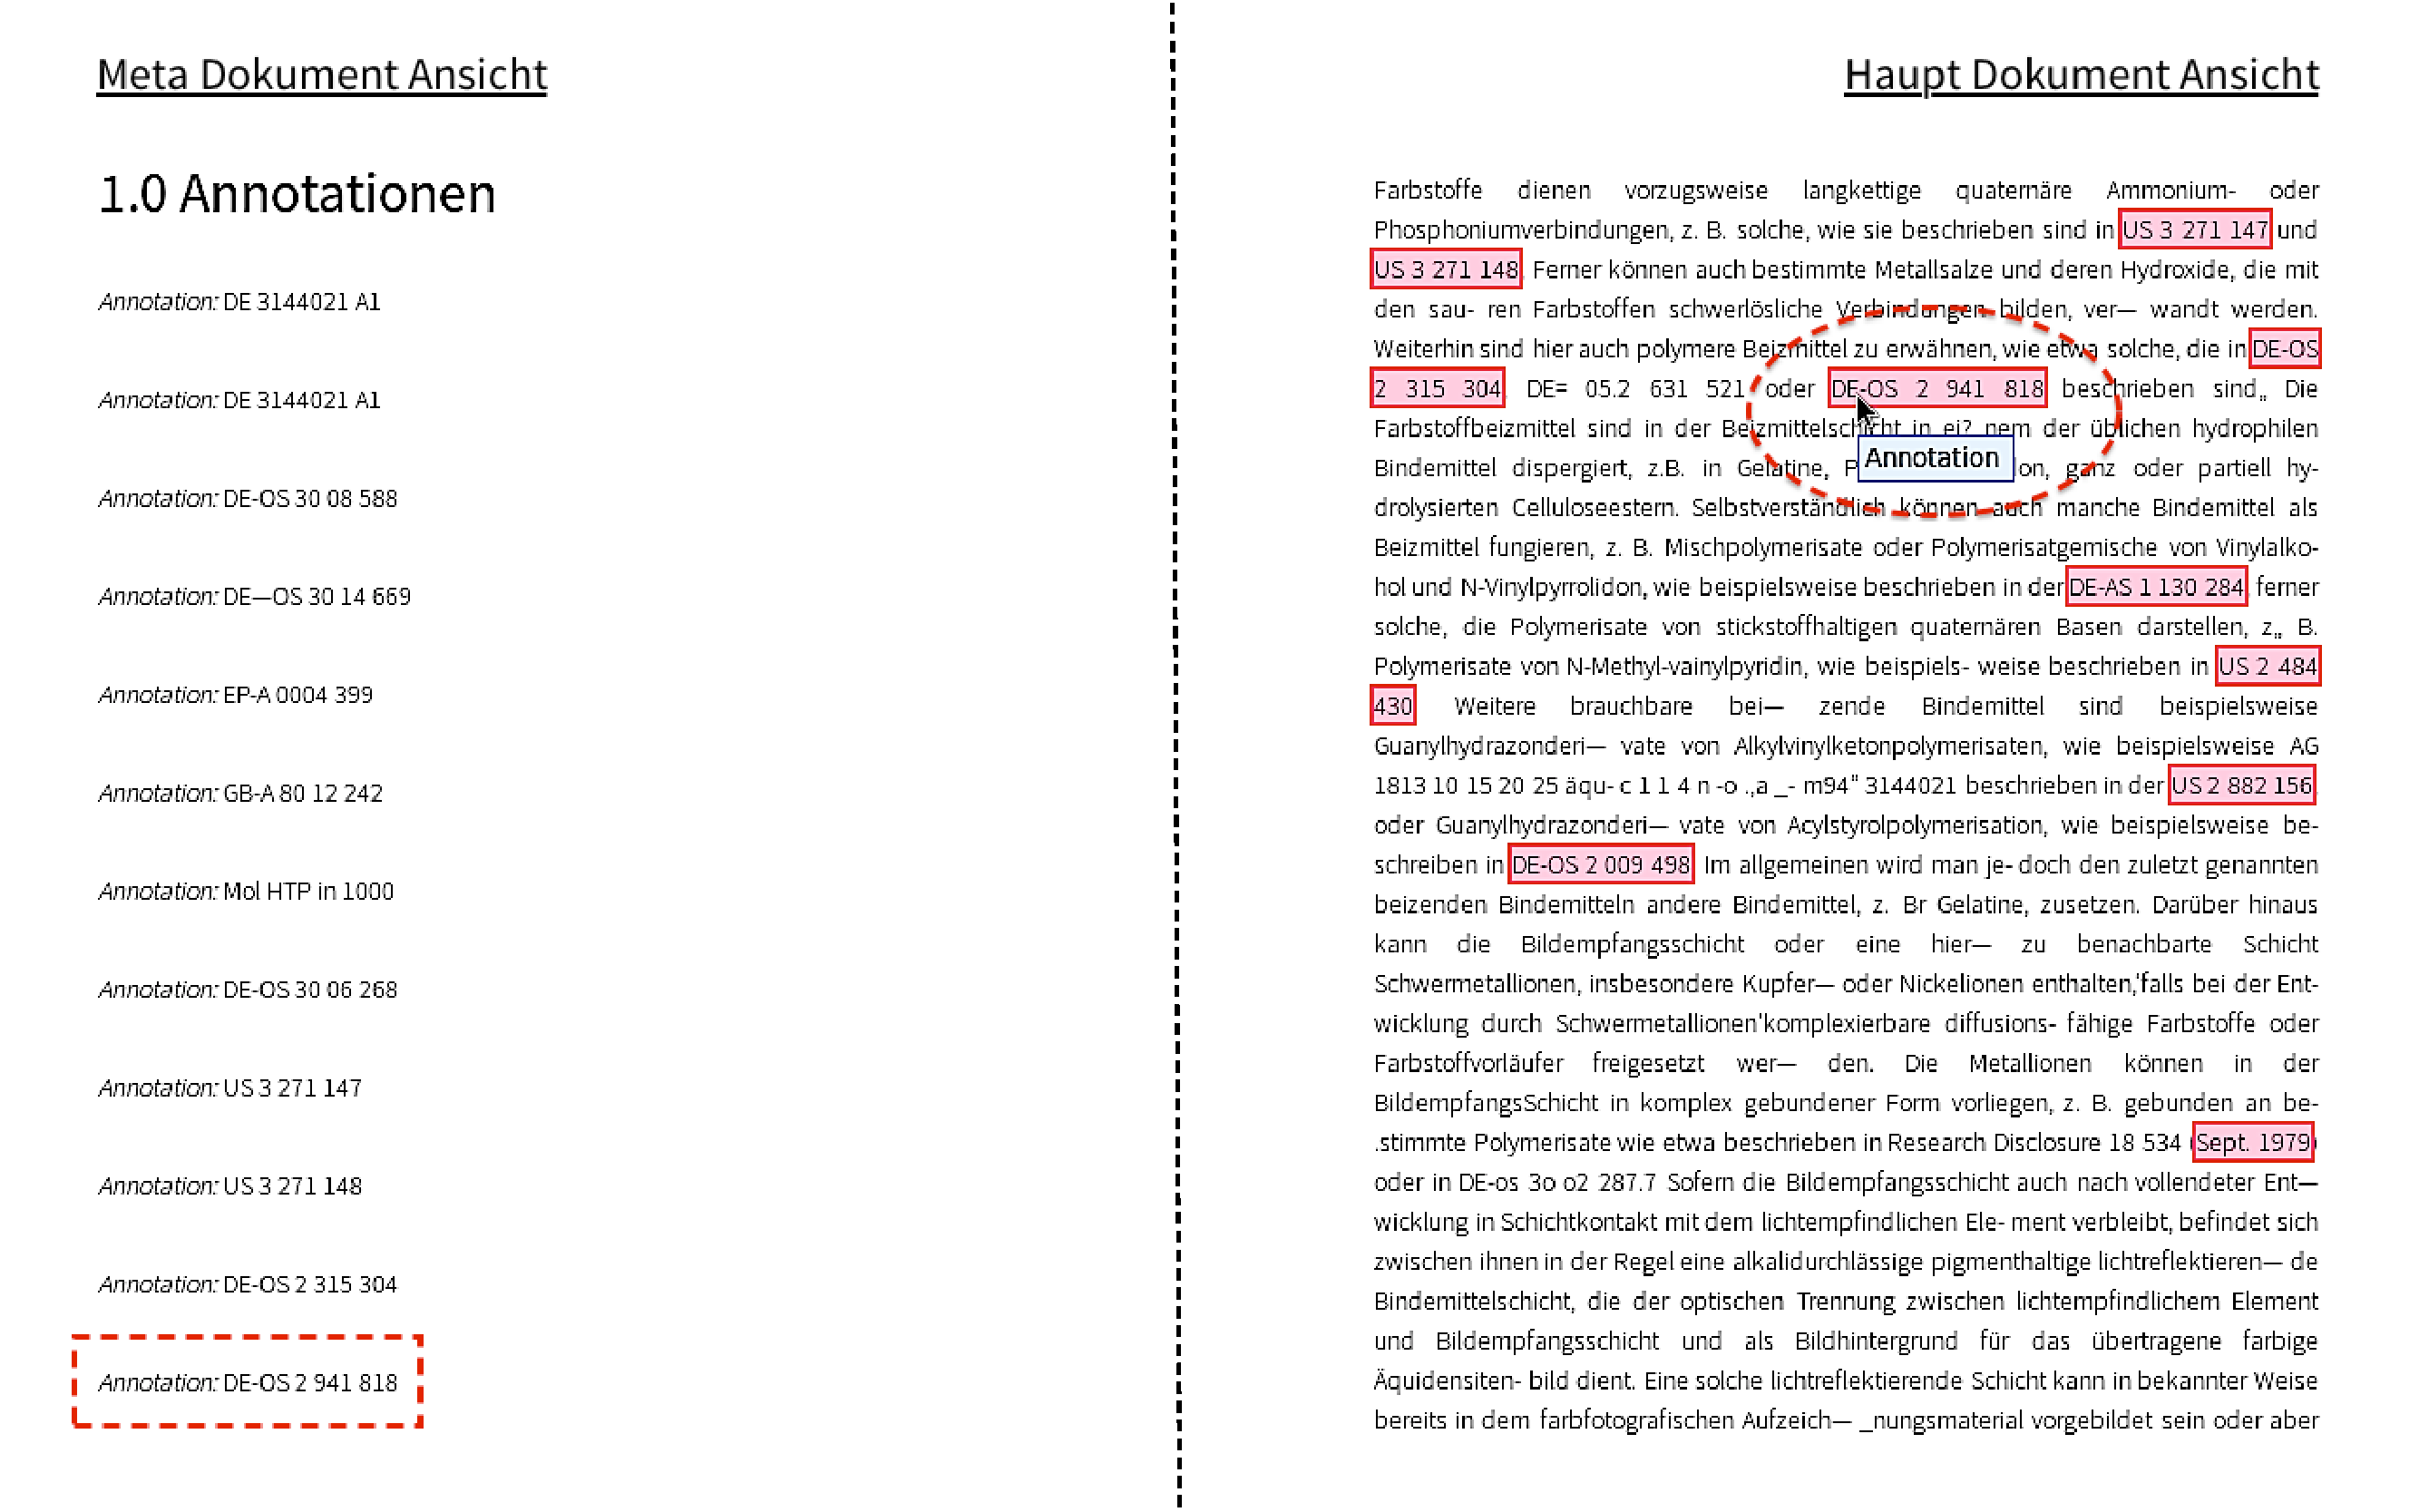
\includegraphics[width=1.45\textwidth]{figures/annotation.png.pdf} }
\caption{ Entnommen aus Screenshots des Prototypen. Es wird dargestellt, wie Annotationen vom Meta Dokument in das Haupt Dokument (über Verweisung) fließen können. Im Haupt Dokument werden bei „mouse over“ alle Annotationen vom gleichen Annotations-Typ „Annotation“ farbig hervorgehoben. Es ist möglich beliebige Annotations-Typen (als Dokumentelement) zu kreieren. }\label{annotation}
\end{figure}
 
\section{Dokumentation von Spray-Modellen}\label{doku-spray}
 
Spray\footnote{~Webseite des Spray Projekts: http://eclipselabs.org/p/spray/} ist ein Forschungsprojekt im Bereich der modellgetriebenen Softwareentwicklung, an der HTWG Konstanz. Spray erstellt Editoren für visuelle domänenspezifische Sprachen (DSL). Das heißt mit Spray können z.B. Diagramme wie Petrinetze, UML, etc. formal definiert werden und aus diesen Definitionen kann ein Editor generiert werden. Mit einem solchen Editor kann dann das jeweilige Diagramm gezeichnet bzw. modelliert werden kann. Vorteil ist, dass durch die Grammatik der visuellen DSL genau spezifiziert ist, welche Verbindungen zwischen den einzelnen Knoten erlaubt sind und welche nicht, d.h. der Diagramm Editor kann zu einem gewissen Grad die Korrektheit des Modells überprüfen.

 
Das heißt, ein mit Spray generierter Editor arbeitet auf einer abstrakteren Ebene -- der Modellebene. Das Modell selbst sollte jedoch auf einer noch abstrakteren Ebene beschrieben werden: in einer natürlichen Sprache. Andernfalls ist es einem Menschen kaum möglich, ein Modell und dessen Zweckbezug, ohne große Hürden, zu verstehen. Einfacher ausgedrückt: das Modell muss dokumentiert werden, damit andere Projektbeteiligte auch etwas damit anfangen können. Man kann also argumentieren, dass Dokumentation in der Abstraktionsebene nochmals über dem eigentlichen Modell liegt, und das Modell um benötigte sprachliche Erklärungen anreichert. Die Dokumentation fügt also explizit den Pragmatismus zum Modell hinzu: für wen, wann und wozu gibt es das Modell?

 
\subsection{Erhoffter Nutzen}\label{}
 
Die hier vorgestellten Konzepte bzw. Prototyp ermöglichen quasi das gleichzeitige Modellieren und Dokumentieren. Die Dokumentationssoftware ist in der Lage, direkt mit dem Modell zu interagieren und daher ist die Dokumentation in einem sehr hohen Maß konsistent. Zudem ist das Dokumentieren dann kein isolierter Prozess mehr „den man machen muss“, sondern gehört zum Arbeitsablauf der Modellierung dazu. Das heißt: Von der Idee bis zum fertigen Modell kann die Dokumentation das Gedankengebäude des Entwicklers sinnvoll unterstützen.

 
Ich persönlich denke, dass sich durch ein solches Dokumentationswerkzeug ein System wie Spray von anderen Lösungen absetzt und daher ein großes Erfolgspotential entwickeln kann. Oder um es etwas drastischer mit den Worten von Dick Brandon zu formulieren:

 
\begin{quote}
 Documentation is like sex: when it is good, it is very, very good; and when it is bad, it is better than nothing. (Dick Brandon)
\end{quote}
 
Gibt es bereits ein solches Werkzeug im Bereich der modellgetriebenen Softwareentwicklung, wo Dokumentation und Modellierung derart integriert werden können und zudem in einem veröffentlichungsbereiten Format vorliegen, welches wissenschaftlichen Standards entspricht?

 
\subsection{Konzeptionelle Umsetzung}\label{}
 
Der vorgestellte Anwendungsfall wurde beispielhaft im hier entwickelten Prototypen umgesetzt. Das Forschungsteam um Spray hat die Software von einer reinen Java/Eclipse Implementierung ins Web gebracht, das heißt die generierten Diagramm-Editoren liegen auch als Webanwendung\footnote{~Momentan liegt die Spray Online Webanwendung nur intern im VPN-Netz der HTWG Konstanz vor.} mit REST-Schnittstelle vor. Der Prototyp selbst ist auch mit Web Standards gebaut und kann daher recht mühelos mit „Spray Online“ interagieren.

 
Es wurde in Wrapper\footnote{~„Wrapper (Software), ein Programm, das als Schnittstelle zwischen zwei anderen Programmen dient“. Aus Wikipedia http://de.wikipedia.org/wiki/Wrapper} entwickelt, der es ermöglicht, den Spray Online Editor in Form eines Dokumentelements anzubieten. Jedes Dokumentelement kann beliebige Ansichten oder Projektionen haben. Hier gibt es zum einen eine Editierungsansicht (dort können DSLs oder Domäneneditoren platziert werden) und zum anderen eine reine Anzeigeansicht (z.B. als Webseite). Das Spray-Dokumentelement bettet den originalen Spray-Editor in Form einen iframes in die Editierungsansicht ein. Der Benutzer kann dann direkt Änderungen an seinem Spray-Modell vornehmen. Wenn der Benutzer die Änderungen speichert, holt sich das Spray-Dokumentelement den aktuellen Zustand des Modells aus der Spray-Persistenz via REST-Schnittstelle. Im Zustand des Modells sind alle Informationen über das Modell gespeichert, wie z.B. die Namen der einzelnen Diagramm-Knoten. Dadurch, dass das Spray-Dokumentelement Zugriff auf die Attribute des Spray-Modells hat, kann im Dokument auf diese Attribute durch Verweisungen zugegriffen werden. Mit diesem Zugriff kann das Dokument mit dem Modell konsistent gehalten werden und es besteht die Möglichkeit, Semantik explizit zu machen, indem zusätzliche Informationen über die Bedeutung des referenzierten Attributes angezeigt werden. Für die Anzeigeansicht holt sich das Spray-Dokumentelement ein svg-Bild des Diagramms -- dieses kann über einen HTTP-Request vom Spray Online Editor abgefragt werden.

 
In Abbildung \ref{sprayanzeigen} ist das Szenario aufgezeigt. Ziel ist es, Attribute aus dem Spray-Modell als Verweis innerhalb des Textes anzuzeigen. Hier im Beispiel soll der Name einer Stelle aus einem Petrinetz im Text referenziert werden.

 
\begin{figure}[h!]
\centering
\advance\leftskip-2.5cm
\fbox{ 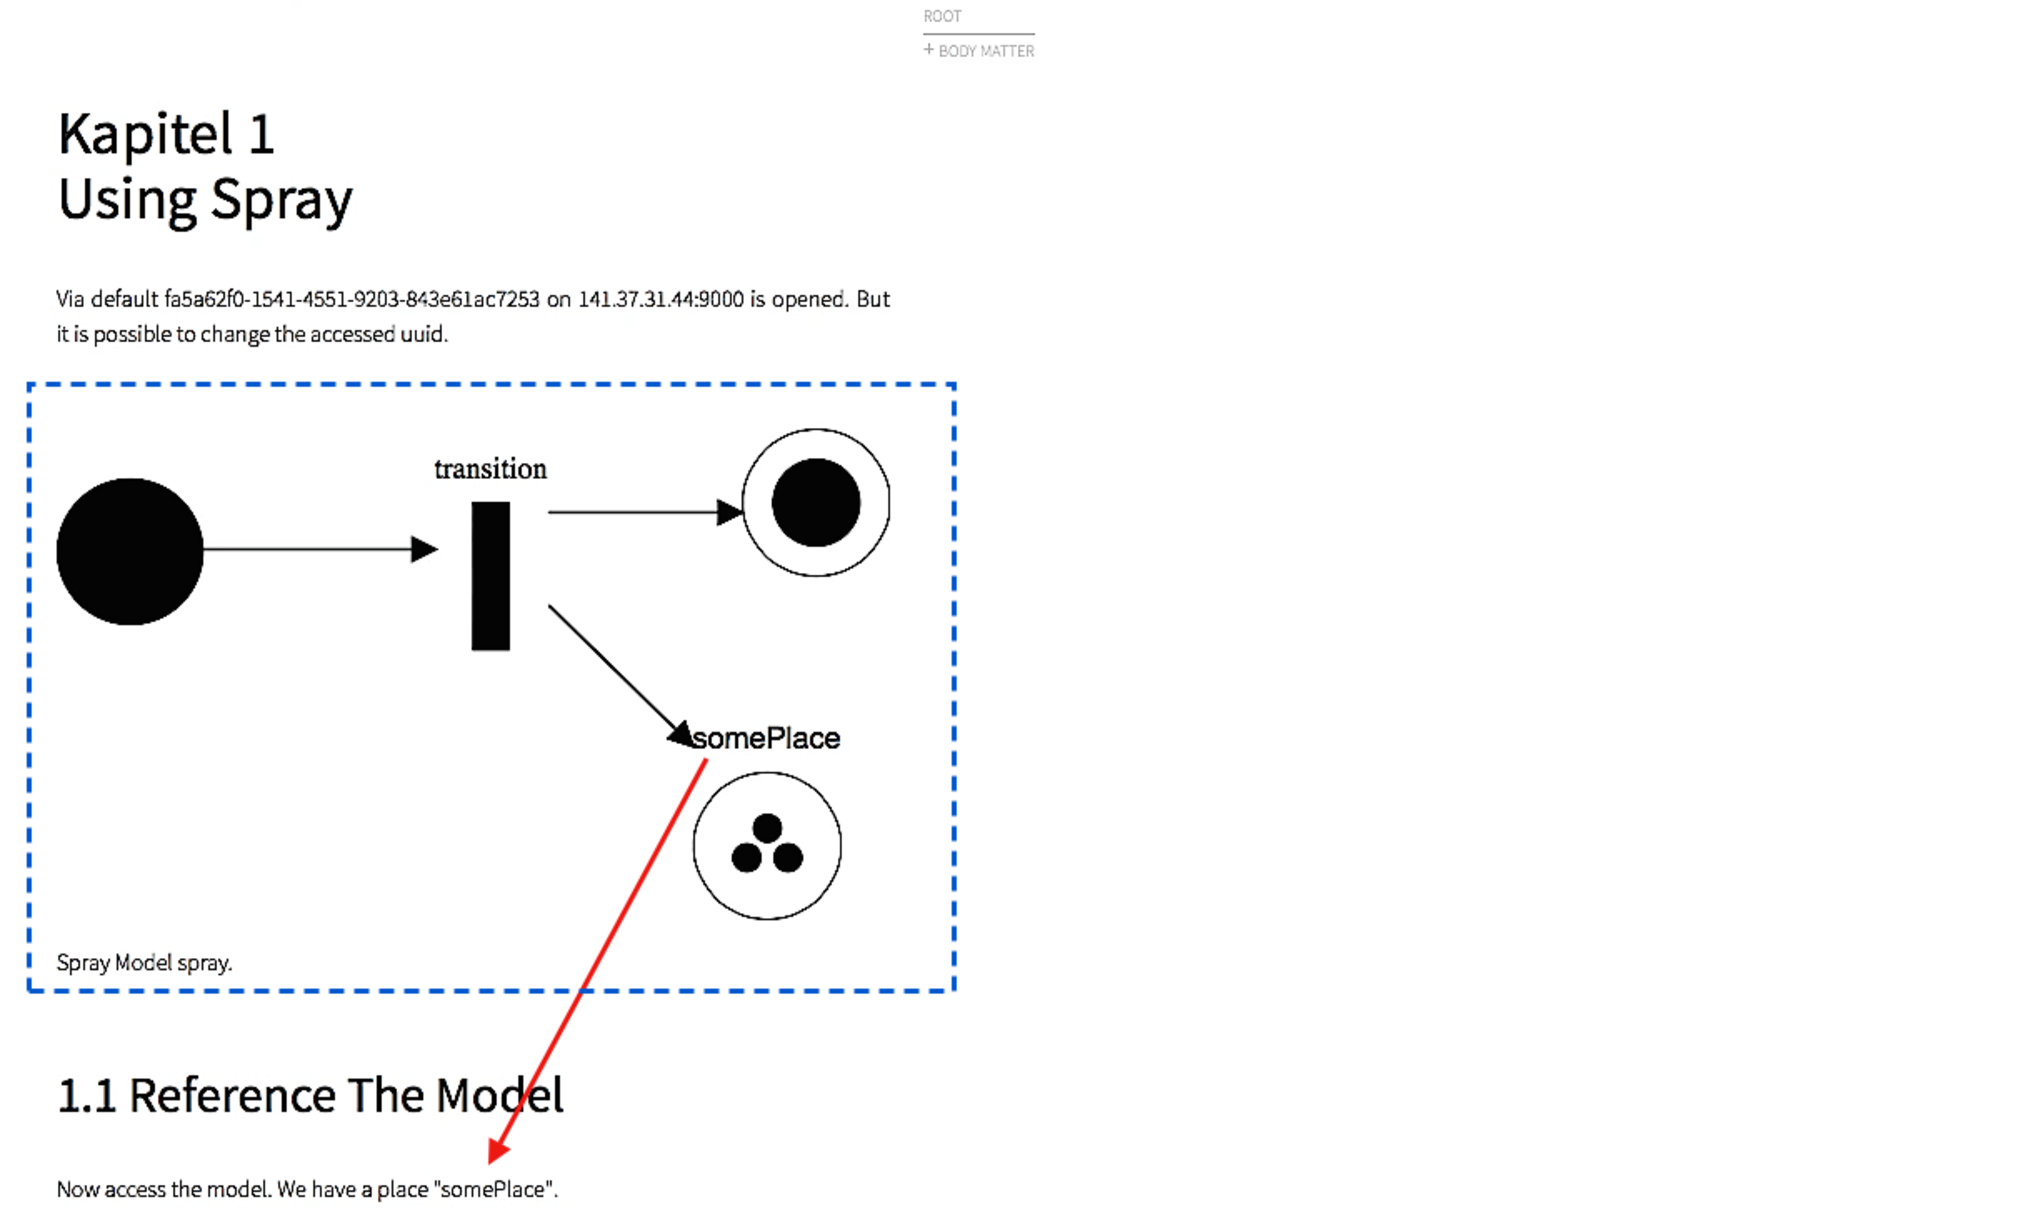
\includegraphics[width=1.45\textwidth]{figures/sprayanzeigen.png.pdf} }
\caption{ Im blau gestrichelten Kasten ist das Spray-Dokumentelement in seiner Anzeigeansicht zu sehen. Szenario: Der Name einer Stelle des Petrinetz-Diagramms soll im Text erwähnt werden (roter Pfeil). }\label{sprayanzeigen}
\end{figure}
 
Wenn der Benutzer das Spray-Dokumentelement anklickt, öffnet sich eine Editieransicht in der das Modell manipuliert werden kann. (Dargestellt auf Abbildung \ref{sprayeditieren}) Dort wird der (1) Domäneneditor „Spray Online“ dargestellt. Der Editor hat ein Petrinetz-Modell geladen, welches vom Benutzer manipuliert werden kann. Das Spray-Dokumentelement kann (2) einen Namen erhalten, um es später beim Verweisen auf das Modell (komfortabel) wieder zu finden. Wenn der Benutzer (3) die Änderungen speichert, holt sie das Spray-Dokumentelement die aktuellen Informationen über den momentanen Zustand des Modells (wie z.B. die Namen der einzelnen Diagramm-Komponenten).

 
\begin{figure}[h!]
\centering
\advance\leftskip-2.5cm
\fbox{ 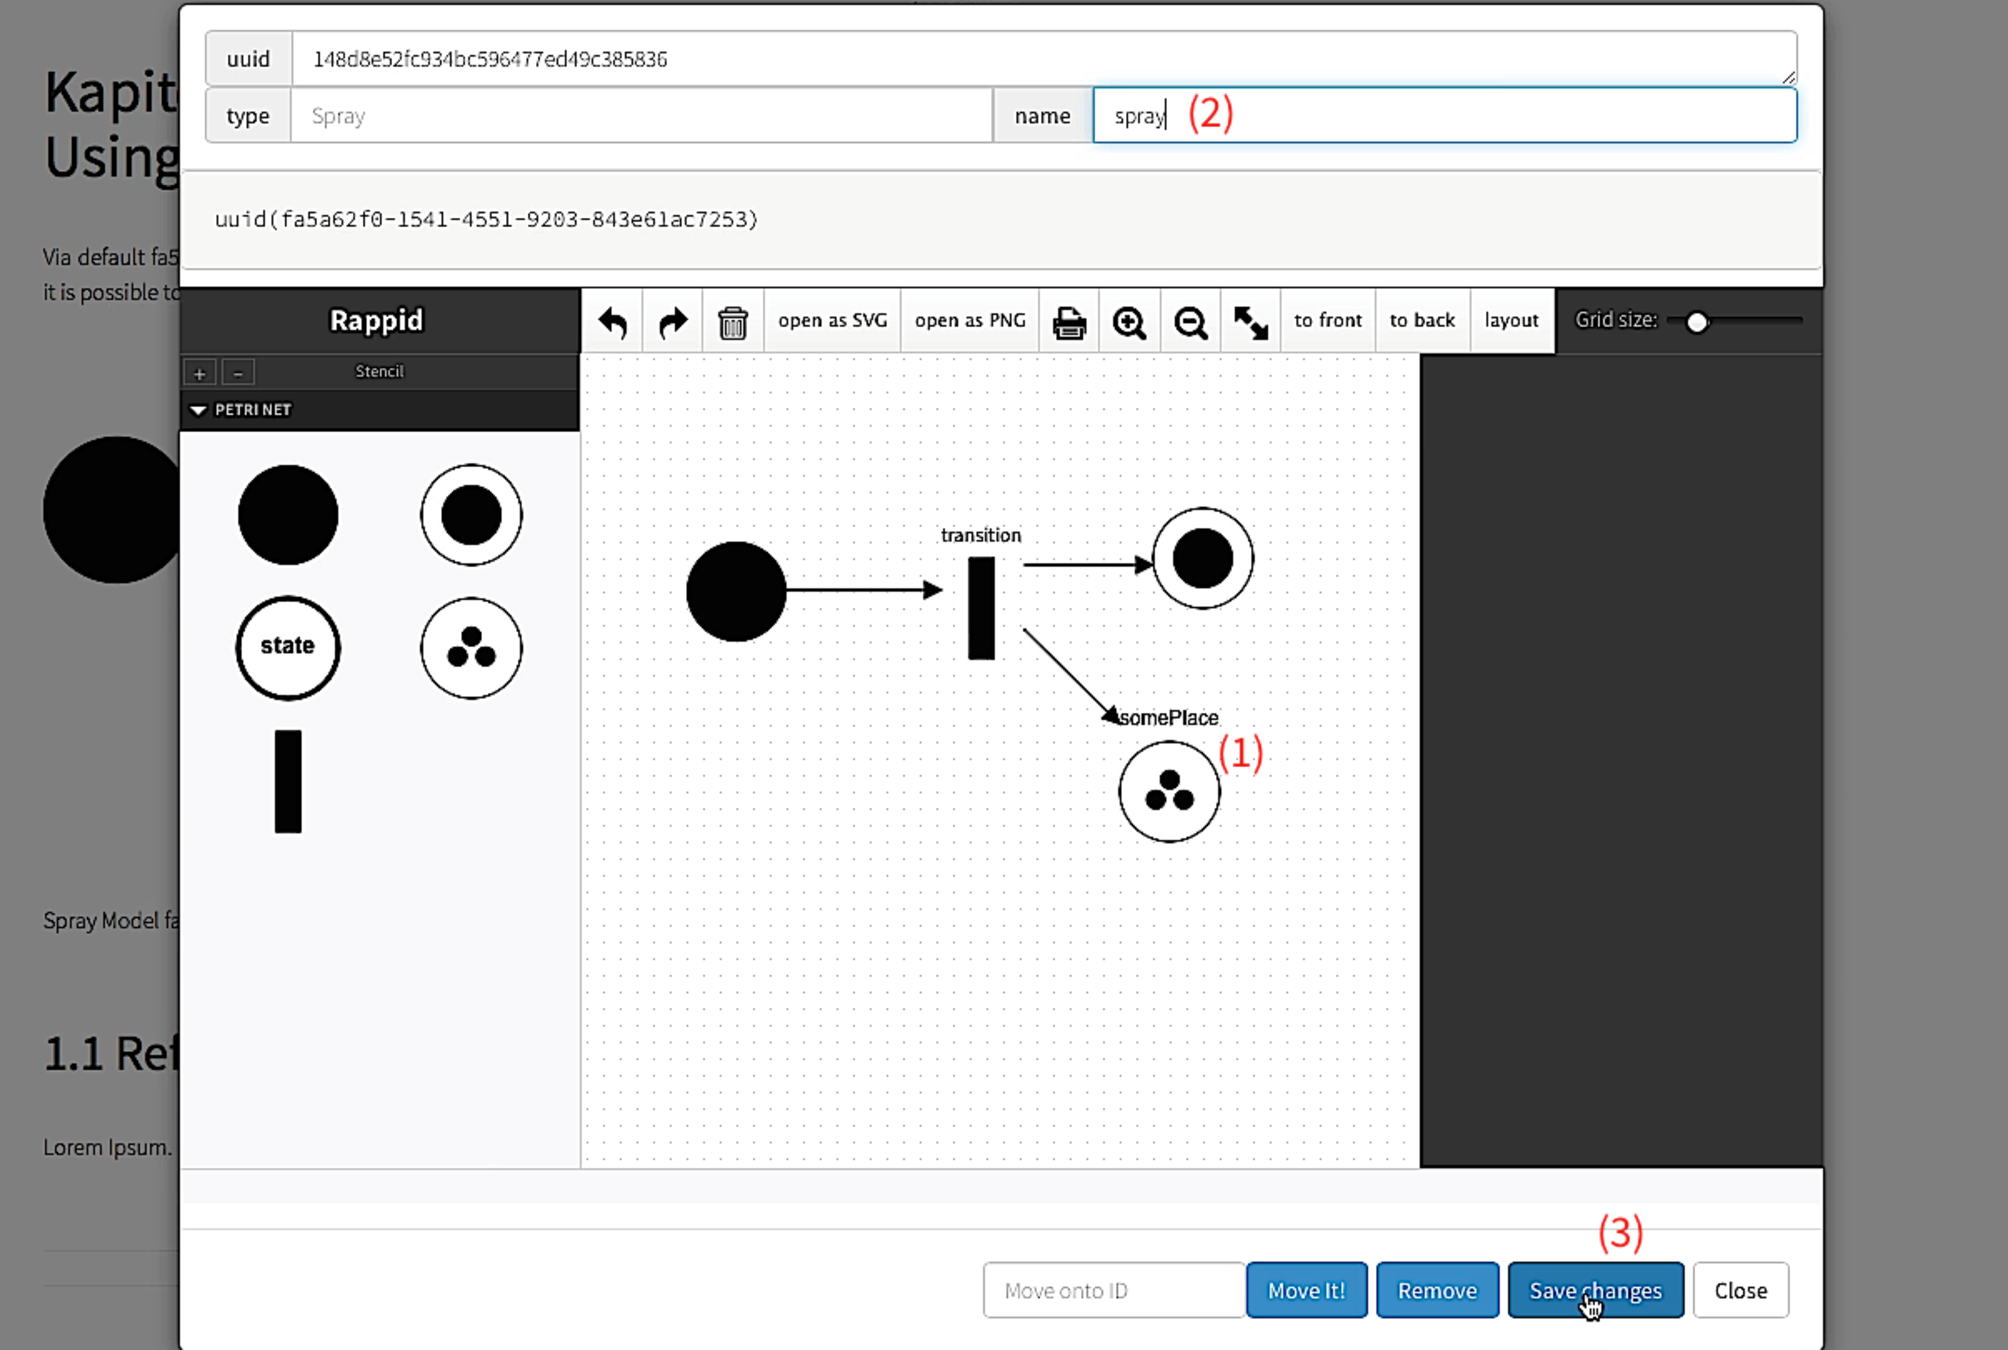
\includegraphics[width=1.45\textwidth]{figures/sprayeditieren.png.pdf} }
\caption{ Ansicht zum Bearbeiten des Spray-Dokumentelement. In (1) ist der Domäneneditor, welcher das Modell in Diagrammform anzeigt und durch den Benutzer manipulierbar macht. Das Modell kann benannt werden für die spätere Verweisung im Text (2). Speichern der Veränderungen (3) veranlassen das Spray-Dokumentelement die aktuellen Modell-Informationen zu laden. }\label{sprayeditieren}
\end{figure}
 
In Abbildung \ref{sprayreferenzieren} wird die Editieransicht eines Abschnitts gezeigt. Dieser Abschnitt soll auf das Modell verweisen, und sich bei Änderungen des Modells selbst aktualisieren zu können. Der Programmausdruck holt sich die entsprechenden Informationen über das Modell direkt beim Spray-Dokumentelement ab. Der rot unterstrichene Teil-Programmausdruck zeigt alle verfügbaren Modell-Informationen (s. Pfeil),  die es gerade über alle Stellen im Petrinetz gibt, an. So kann sich der Autor auch eine einzelne Stelle des Petrinetzes herauspicken und ihren (aktuellen) Namen abfragen. Abbildung \ref{sprayanzeigen} zeigt das Resultat.

 
\begin{figure}[h!]
\centering
\advance\leftskip-2.5cm
\fbox{ 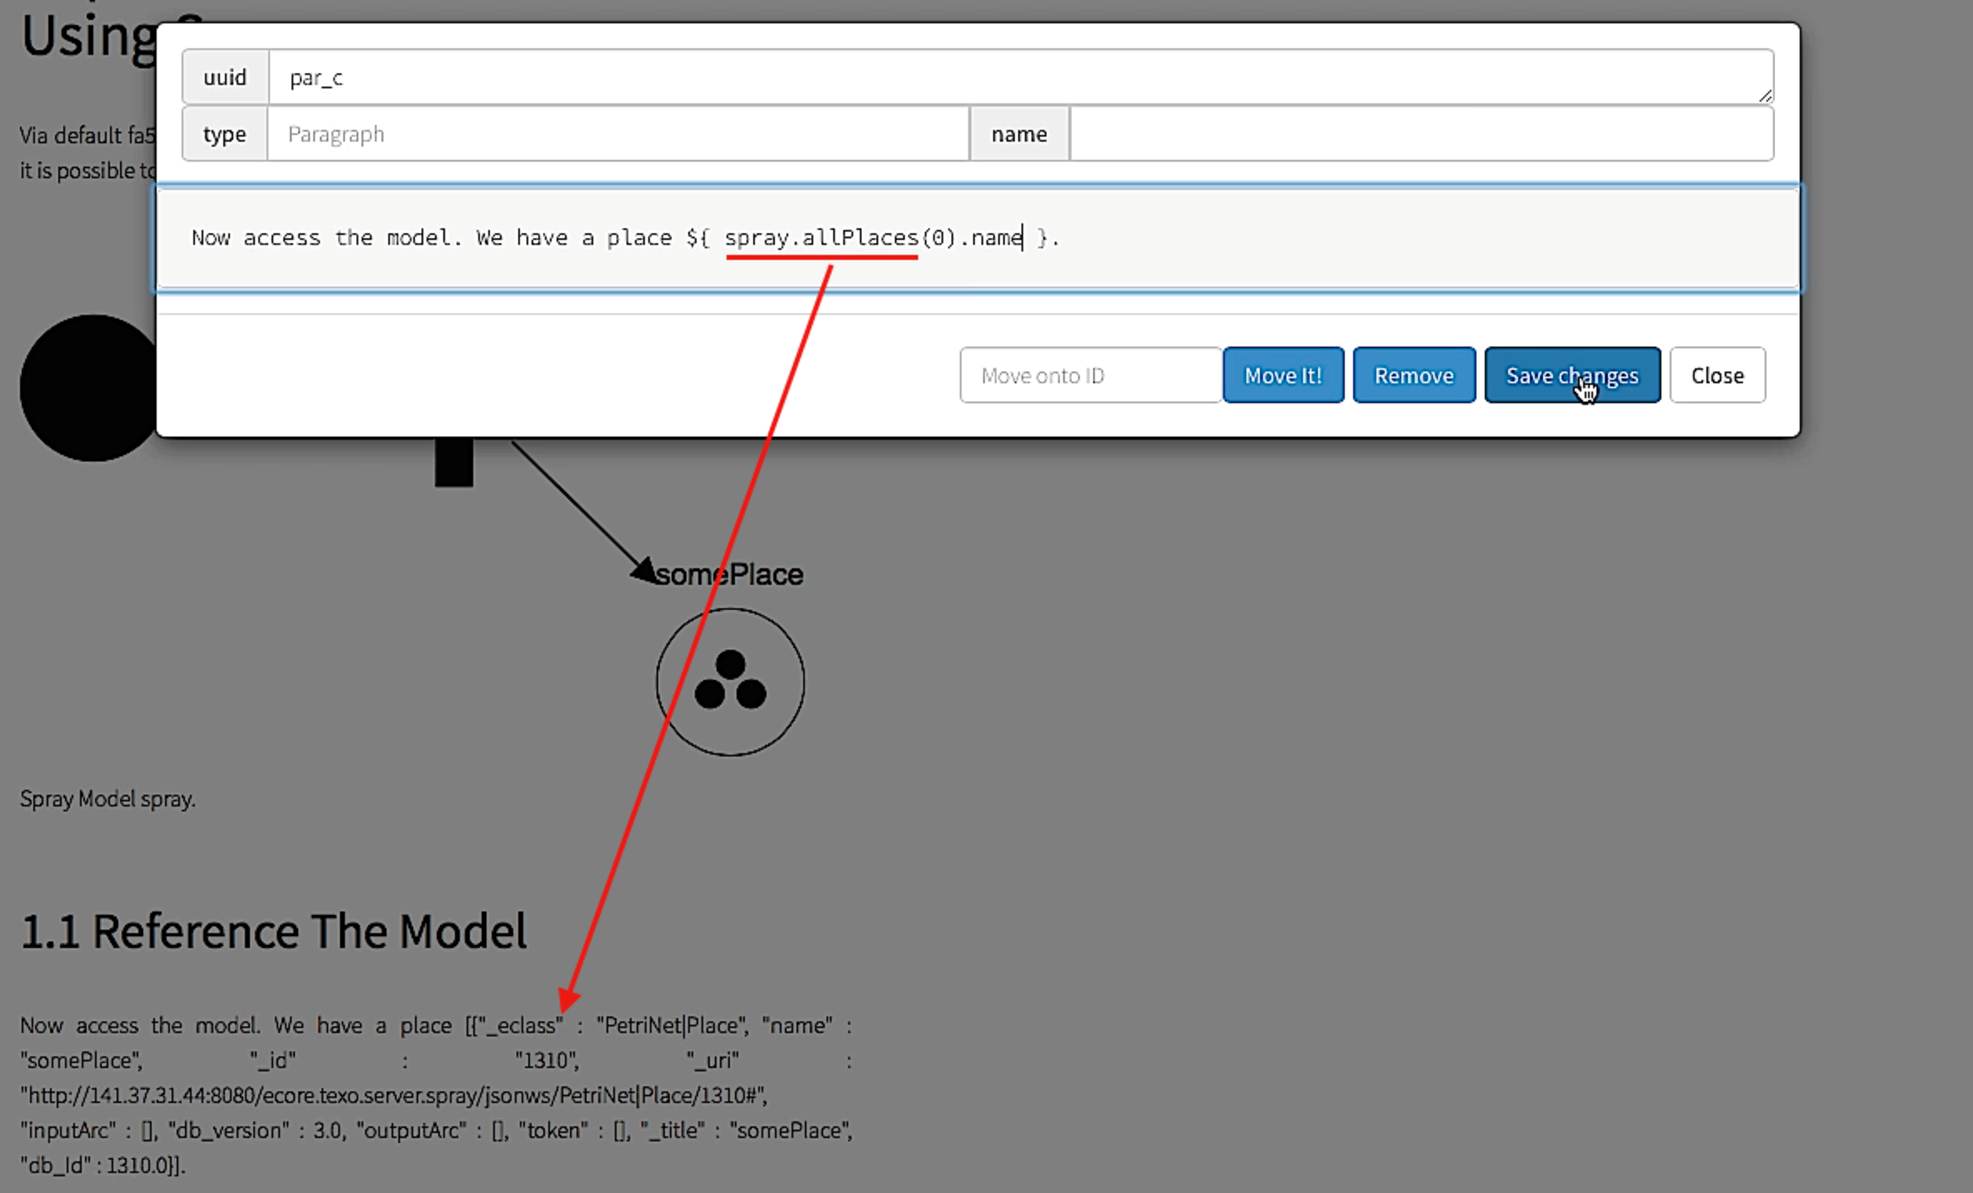
\includegraphics[width=1.45\textwidth]{figures/sprayreferenzieren.png.pdf} }
\caption{ Hier wird auf das Spray-Dokumentelement verwiesen. Mit einem Programmausdruck kann der aktuelle Zustand des Modells abgefragt werden und bei Bedarf auf einzelne Attribute verwiesen werden. Bei Modelländerungen (z.B. Umbenennungen eines Diagrammknotens) bleibt der Text konsistent. }\label{sprayreferenzieren}
\end{figure}
 
\section{Transformation in andere Formate}\label{transformation}
 
Dokumente in andere Formate zu überführen war schon immer notwendig, und in modernen Zeiten immer wichtiger. Beispielsweise werden von wissenschaftlichen Berichten (wie Diplomarbeiten) Manuskripte angefertigt. Diese werden später vom Verleger überarbeitet und in ein Buch (oder eBook) gesetzt, vgl. \citep{DIN1422-1}. Daran hat sich nichts geändert, nur dass die Schreibmaschine durch ein Textverarbeitungsprogramm ersetzt wurde und der Vorgang dadurch etwas komfortabler geworden ist.

 
Für Format Transformationen gibt es in jüngster Zeit auch noch andere Anwendungsgebiete. Beispielsweise möchte man historische Dokumente digitalisieren und mit möglichst vielen Zusatzinformationen anreichern (vgl. Abschnitt \ref{uima-cas-kapitel}). Es gibt auch noch andere Szenarien, in denen Transformationen in u.U. vollkommen unterschiedliche Formate nützlich sein kann:

 
\begin{itemize}

\item Format zur Speicherung von Dokumente in digitalen Langzeitarchiven.
\item Überführung von Dokumenten mit alten Layout-Konventionen in die Neuen.
\item Dokumente gleichzeitig sowohl für legacy Software als auch für aktuelle Software zugänglich halten.
\item Ein Dokument für andere Arbeitsgebiete aufbrechen: wie z.B. Knowledge Discovery, Semantic Web.
\item Ein Dokument auf ein bestimmtes Publikum spezialisieren oder in eine andere Dokumentklasse überführen (Journal Artikel in eine Präsentation transformieren).
\end{itemize}
 
Hier kommt der abstrakte Syntaxbaum (AST) ins Spiel: Ein AST ist innerhalb eines Übersetzers eine Zwischenrepräsentation für ein Programm, woraus schlussendlich Maschinencode produziert wird -- Details in Abschnitt \ref{ast-sec}. Hier wird direkt auf dem AST gearbeitet (Projektionseditor). Der AST repräsentiert zudem auch direkt das Modell des Dokuments und jedes Dokumentelement hat wiederum Wissen über seine Domäne. Es sind also genügend Informationen vorhanden, um quasi beliebige Formate zu produzieren. Es muss somit nur eine weitere Projektion zum AST hinzugefügt werden (als Template), damit ein entsprechendes Format erzeugt werden kann. Das heißt: Statt klassisch Maschinencode zu produzieren, kann hier auch ein anderes Dokumentformat produziert werden, wie z.B. \citep{NISO} konformes XML, XMI für CAS Objekte, ePub, etc.

 
Hier wurde beispielhaft, neben der HTML-Projektion mit Editier-Funktion, LaTeX-Code als Projektion umgesetzt. Aus diesem LaTeX-Code kann wiederum ein (paginiertes) PDF generiert werden. Dies wird auch so genutzt, um diese Masterarbeit zu schreiben -- siehe Abschnitt \ref{wiss-dok-abschnitt}.

 
\chapter{Entwicklung des Prototypen}\label{}
 
Um die wissenschaftlichen Fragen zu beantworten, wurde als Methode die Entwicklung eines Prototypen gewählt. Anhand des Prototypen können Aussagen getroffen werden, ob die vorgestellten Ideen und Konzepte tragfähig sind. Zudem können die Konzepte verfeinert und Impulse für neue Ideen bzw. Theorien gefunden werden.

 
Zunächst wird das allgemeine Vorgehen erläutert. Hierbei stehen die für den Prototyp aufgestellten Test-Spezifikationen im Mittelpunkt. Dann folgen Basiskonzepte, die dem Prototypen inne wohnen. Daraus ergibt sich eine Architektur, die von Grob zu Detailreich beleuchtet wird. Am Ende des Kapitels wird der erreichte Funktionsumfang diskutiert und mit einer kleinen Statistik über den Codeumfang des Prototypen abgeschlossen.

 
Der Quellcode \citep{HodappScaltex} ist auf GitHub öffentlich zugänglich und wird via Zendodo.org zitierbar gemacht, d.h. Version 0.6.0 des Prototypen erhält eine DOI (digital object identifier) und liegt im Langzeitarchiv von Zenodo. Im Quellcode ist eine README Datei, welche als Anhang für die Masterarbeit dient. Dort ist u.a. beschrieben, wie die Software installiert werden kann, welche Releases (Meist Zwischenstände für Vorträge) es gegeben hat.

 
\section{Vorgehen}\label{}
 
Als Entwicklungsmethode wird das Behavior-Driven development (BDD) eingesetzt, welches von \citep{North} geprägt wurde. (Unit) Tests werden dort in Form von Spezifikationen verfasst. Jede Spezifikation soll ein bestimmtes Verhalten der Software dokumentieren und verifizieren. Das Framework ScalaTest\footnote{~Tests als Spezifikationen aus der Dokumentation von ScalaTest: http://www.scalatest.org/user\_guide/tests\_as\_specifications} bietet die Möglichkeit, nach BDD Softwaresysteme zu entwickeln. Die Aktoren-Implementierung des Prototypen wird mit ScalaTest getestet.

 
Bei jedem git push auf GitHub wird automatisch Travis CI aktiv. Hierbei handelt es sich um eine Continuous Integration Platform, welche die richtige Umgebung zum Ausführen von ScalaTest\footnote{~Travis CI für das Git Repositorium des Prototypen: https://travis-ci.org/themerius/scaltex-2} einrichtet. Es werden automatisch die benötigen Scala Abhängigkeiten herunterladen und kompiliert, sowie eine CouchDB für die Tests zur Persistenz bereitgestellt. Ob die Tests fehlschlagen oder glücken, wird in einem Protokoll festgehalten.

 
\subsection{Getestete Spezifikationen}\label{}
 
Hier sind die 41 Spezifikationen die an den Prototypen gestellt wurden aufgelistet. Die Spezifikationen sind in englischer Sprache gehalten, da dies die übliche Weise ist, Software zu dokumentieren. Die Spezifikationen sind so formuliert, dass sie möglichst selbsterklärend sind. Nachfolgend die Ausgabe von ScalaTest:

 
\begin{verbatim}
RootSpec:
The Root Actor
- should hold topological informations about the document
- should digg for the firstChilds
- should digg for the next references
- should be able to calculate the correct order of the document elements
- should be able to insert (new) elements and remove elements from topology
- should setup the document actors with a given topology
- should be able to initiate the Update through the entire document
- should pass messages to the selected id

RemoveElementSpec:
Remove of a non-leaf
- should repair the topology and put the removed subtree into the graveyard
Remove of a leaf
- should repair the topology and put the removed element into the graveyard

MoveElementSpec:
Move of a non-leaf
- should change the topology (hang a entire subtree to a destination)
- should change the topology (hang a entire subtree to a destination II)
- should move the entire subtree into another hierarchy level
Move of a leaf
- should change the topology and recreate the actor at the desired position
- should also work if moved to a position of a first child

ReportSpec:
A REPORT document meta model element
- should save it's unique id into it's state
- should be able to change it's current assigned document element
- should be able to obtain a reference to the next actor
- should send update to the next actors
- should have a content (source, representation and result from evaluation)
- should send deltas when the topology changes
  + When a new element is inserted after a leaf 
  + Then updater should receive a delta (topology change set) 
  + And the new-elem should register itself to root 
  + When a new element is inserted after a non-leaf 
  + Then updater should receive a delta to the lastChild 
  + When a new element is inserted as first child (extend hierarchy) 
  + Then updater should receive a delta 
A element with a variable (short) name
- should be part of the base actor state
- should be changeable

OutlineSpec:
The SECTION document elements
- should have `title` and `numbering` properties
- should change the `title` attribute when the content changes
- should be able to discover it's (primary) section number
- should be able to discover it's (secundary) section number
- should be able to discover it's (tertiary) section number

TableOfContentsSpec:
The TableOfContents element
- should ask every Chapter and *Section within BodyMatter

InterpreterSpec:
A INTERPRETER
- should evaluate a string which contains scala code
- should return None if evaluation fails

DiscoverReferencesSpec:
The References Discovery
- should find all ActorRefs within a Sting
- should generate code of the classes the user may use
- should collect the complete code and put the evaluated repr into contentRepr
Unified content
- should be an array with the expression details

CouchDbSpec:
Root
- should be able to load a document from CouchDB persistance
- should NOT integrate _id and _rev from CouchDB into the topology
- should persist the topology on changes
Each such created element
- should aquire it's state from persistance 'to life'
- should save state, if changed, back to persistance
- should save state if it's not persisted yet
\end{verbatim}
 
\section{Basiskonzepte}\label{basiskonzepte}
 
Der Prototyp versucht die Anforderungen aus Abschnitt \ref{anforderungen-sec} umzusetzen. Hier nochmals kurz in Stichpunkten zusammengefasst:

 
\begin{enumerate}

\item Abstraktion für Dokumentelemente
\item Domänenspezifische Inhalte in Dokumentelementen
\item Reichhaltige Verweisungen für explizite Semantik und mehr Konsistenz
\item Metamodell definiert erlaube Dokumentelemente
\item Projektionseditor für Dokumente, mit Web Standards umgesetzt
\end{enumerate}
 
(1) Es ist möglich ein Dokument als abstrakten Syntaxbaum darzustellen, wobei jeder Knoten einem Dokumentelement entspricht. (2) Jedes Dokumentelement kann Teile seiner Domäne in den Attributen abspeichern und einen Domäneneditor, der im Browser ausgeführt wird, bereitstellen. (3) Dokumentelemente können durch Nachrichtenaustausch Attribute eines anderen Dokumentelements abfragen und in den eigenen Kontext einbauen. Diese Abfragen werden in der Programmiersprache Scala notiert und von einem Scala-Interpreter ausgewertet. (4) Jedes Dokumentelement implementiert eine Scala Klasse, wodurch es repräsentiert wird. Der Scala-Interpreter kann diese Klassen instanziieren und ausführen. Das Resultat kann z.B. an ein anderes Dokumentelement geschickt werden. (5) Nachrichten aus einem Websocket können zum abstrakten Syntaxbaum geleitet werden, und umgekehrt. Dieser kann darauf reagieren bzw. entsprechende Maßnahmen ausführen. Beispielsweise kann er sich selbst modifizieren (Knoten hinzufügen/entfernen) oder analysieren (Neue Attribute der Knoten entdecken, wie z.B. Benummerungen zu Abschnitten hinzufügen).

 
Bedient wird die Textverarbeitung über den Browser. Diese stellt den abstrakten Syntaxbaum des Dokuments übersichtlich dar. Der Benutzer arbeitet also direkt mit abstrakten Syntaxbaum, bekommt jedoch nur ausgewählte bzw. relevante Attribute als „konkrete Syntax“ angezeigt. Der Autor bekommt also eine möglichst komfortable Ansicht des Dokuments. Wenn er auf ein Dokumentelement klickt, wird ein Fenster geöffnet. Dort werden nähere Informationen zum Dokumentelement eingeblendet und das Dokumentelement kann dort bearbeitet werden. In dieser Ansicht können neben textuellen Eingaben (z.B. in Form von DSLs) auch domänenspezifische Editoren (wie z.B. ein chemischer Moleküleditor) angezeigt werden.

 
\section{Architektur}\label{}
 
Auf Abbildung \ref{architektur-fig} ist eine Übersicht über die Architektur des Prototypen. Der Dreh- und Angelpunkt ist das Dokumentmodell (vgl. Abschnitt \ref{dokumentModell}), mit dem der Autor quasi direkt kommunizieren kann. Das Dokumentmodell wird von seinem Metamodell (vgl. Abbildung \ref{metamodell}) abgeleitet, dort sind u.a. die einzelnen Dokumentelemente definiert.

 
Jedes einzelne Dokumentelement, also jeder Aktor, persistiert bei Änderungen des Zustandes diesen in CouchDB. CouchDB ist eine dokumentenorientierte NoSQL-Datenbank, welche JSON-Objekte speichern kann. Eine Besonderheit der Datenbank ist, dass jede Änderung am JSON-Objekt mit einer neuen Version versehen wird, d.h. es ist möglich die Entstehungsgeschichte eines jeden Dokumentelements nachzuvollziehen. Es ist also möglich, ein Dokument zerstörungsfrei zu erstellen. Neben der Versionskontrolle ist die REST-Schnittstelle zur Datenbank ein Basiskonzept von CouchDB, s. \citep{Anderson}.

 
Xitrum ist ein controller-first Web Framework, geschrieben in Scala. Die Aufgabe von Xitrum ist es, Websockets für die Kommunikation mit dem Browser bereitzustellen und statische Dateien, wie HTML-Templates, CSS, JavaScript oder Bilder auszuliefern. Das Dokumentmodell hat einen Update Aktor, welcher die Änderungen vom Browser bzw. vom Modell handhabt. Der Update Aktor kann mit mehreren Websockets gleichzeitig sprechen. Dies ermöglicht es, dass mehrere Browser das gleiche Dokument betrachten können und live die Änderungen der anderen Parteien mitbekommen. Jeder Browser ist mit einem Websocket verbunden.

 
\begin{figure}[h!]
\centering
\advance\leftskip-2.5cm
\fbox{ 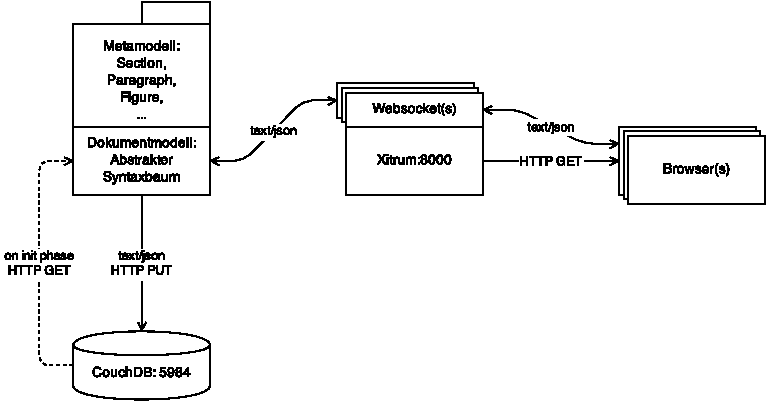
\includegraphics[width=1.45\textwidth]{figures/architektur.svg.pdf} }
\caption{ Die Architektur des Prototypen. Die Pfeile stellen die Kommunikation zwischen den einzelnen Komponenten dar. Die Kommunikation läuft zum einen über das Websocket-Protokoll und zum anderen über HTTP-Calls. Die Daten werden stets als JSON-String übertragen, außer bei der Auslieferung der statischen Daten durch Xitrum. Der gestrichelte Pfeil ist eine einmalige Kommunikation, die nur zum Initialisieren des Aktor Systems (bzw. abstrakten Syntaxbaumes) verwendet wird. Bei der Initialisierung holt sich jedes Dokumentelement den gespeicherten Zustand aus der Datenbank. Wenn sich der Zustand eines Dokumentelements ändert, wird dies in der Datenbank als neue Version gespeichert. }\label{architektur-fig}
\end{figure}
 
\subsection{Wurzel Aktor}\label{}
 
Der Wurzel oder Root Aktor enthält die Topologie des Dokuments. Hier werden also alle Aufgaben, die mit der Topologie zusammenhängen, verarbeitet. Der Root Aktor hat als einziger Aktor die Gesamtübersicht über das Dokument. Zwar speichert jeder Dokumentelement-Aktor seine lokalen Beziehungen (Kinder, Geschwister), aber diese werden nicht in die Datenbank geschrieben. Somit wird verhindert, dass durch eine Wiederherstellung einer Version eines Dokumentelements irgendwelche Topologie-Lücken aufgerissen werden. Nur der Root Aktor speichert topologische Informationen in der Datenbank ab. Wenn Versionen des Root Aktors wiederherstellt werden, wird somit ausschließlich die Topologie wiederhergestellt. Das heißt, die Topologie kann unabhängig von den aktuellen Inhalten der einzelnen Dokumentelemente restauriert werden. Stichwortartig zusammengefasst:

 
\begin{itemize}

\item Enthält die (gesamte) Topologie des Dokuments
\item Persistiert die Topologie in die Datenbank
\item Kann Topologie-Änderungen initiieren (wie z.B. hinzufügen, entfernen und verschieben von Knoten)
\item Kann Topologie-Informationen bereitstellen (wie z.B. Position der einzelnen Dokumentelemente)
\item Ist der Einstiegspunkt für das Dokument
\end{itemize}
 
\subsection{Basis Aktor}\label{}
 
Der Basis Aktor repräsentiert einen Knoten im abstrakten Syntaxbaum. Er enthält eine Instanz einer Scala Klasse, welche das Dokumentelement mit all seinen Attributen und Methoden beschreibt. Der Basis Aktor trägt also das Dokumentelement quasi huckepack. Der Basis Aktor verwaltet die Nachrichtenkommunikation mit den anderen Aktoren und hält Beziehungen zu seinen Kindern (insbesondere dem ersten Kind) und seinen Geschwistern (insbesondere der Nachfolger). Der Basis Aktor kann bei Änderungen eine Analysephase des gesamten abstrakten Syntaxbaumes auslösen. Dort werden die Dokumentelemente aufgerufen zu überprüfen, ob noch alle Attribute aktuell sind. Beispielsweise kann ein Abschnitt-Dokumentelement seine Benummerung nochmals überdenken. Nochmals in Stichworten:

 
\begin{itemize}

\item Ist ein Knoten des abstrakten Syntaxbaumes
\item Trägt eigentliche Dokumentelemente (mit ihrem Domänenwissen) huckepack
\item Verwaltet die Nachrichtenkommunikation
\item Kennt die lokale Topologie des Dokuments (sein erstes Kind, sein nächstes Geschwister)
\item Bei Änderungen wird eine Analysephase ausgeführt, die auch an das Dokumentelement getragen wird
\end{itemize}
 
\subsection{Metamodell erweitern}\label{metamodell-impl}
 
Ein Teil des Metamodells sind die Dokumentelement Definitionen. Hier wird spezifiziert, welche Dokumentelemente im eigentlichen Dokumentmodell vorkommen dürfen. Weiter wird dort spezifiziert, welche Eigenschaften das Dokumentelement besitzt. Jedes Dokumentelement implementiert das gleiche Interface:

 
\begin{verbatim}
class Figure extends DocumentElement {


  // (1) Attribute
  this.state.title = ""
  this.state.numbering = ""


  // (2) Analysephase
  def _gotUpdate(actorState: Json[_], refs: Refs) = {
    // ...
    super._gotUpdate(actorState, refs)
  }


  // (3) Analysephase
  def _processMsg(m: M, refs: Refs) = {
    // ...
  }


}
\end{verbatim}
 
Im o.g. Quelltext wird ein Dokumentelement „Figure“ (Abbildung) spezifiziert. Es hat (1) ein Menge an Attributen festgelegt, die während der z.B. der Analysephase ändern können. Wenn der Basis Aktor über Änderungen benachrichtigt wird, teilt er das über Methode (2) auch dem Dokumentelement mit. Es erhält Zugriff auf den Zustand des Basis Aktors (hier ist z.B. contentSrc gespeichert, also die rohen Eingaben des Autors) und auf die Referenzen die der Aktor zu anderen Aktoren pflegt. Auf diese Weise kann das Dokumentelement Anfragen an andere Aktoren bzw. Dokumentelemente, im Form von Nachrichten, stellen. Zudem kann es vorkommen, dass es Nachrichten gibt, die direkt an das betreffende Dokumentelement gerichtet sind, diese werden in (3) verarbeitet. Beispielsweise kann Methode (2) eine Nachricht an alle anderen Abbildungen schicken, um ihre korrekte Benummerung herauszufinden. Diese Nachricht würde bei jeder anderen Abbildung in Methode (3) zur weiteren Verarbeitung landen.

 
Beliebige weitere Methoden, die für das Dokumentelement bzw. dessen Domäne nützlich sein könnten, können an diese Scala Klasse hinzugefügt werden. Das ermöglicht den Aktoren reichhaltige Verweisungen untereinander durchzuführen. Es wird also ermöglicht, dass ein Dokumentelement aus den Attributen eine Information berechnen kann und diese an den anfragenden Aktor weitergibt.

 
\subsection{Verweisungen auflösen}\label{verweise-aufloesen}
 
Reichhaltige Verweisungen sind ein grundlegendes Konzept des Prototypen. Hieraus entstehen neben den üblichen Verweisungen, wie man sie aus wiss. Dokumenten kennt (Verw. auf Abbildungen, Abschnitte oder Literatur), neue Möglichkeiten für Semantik und Konsistenz.

 
Dokumentelemente liegen als Scala Klasse vor und eine Verweisung greift darauf direkt zu. Das heißt innerhalb eines Textes wird mit einem Scala Programmausdruck notiert, auf welches Attribut oder Methode zugegriffen werden soll und welches Dokumentelement adressiert werden soll. Prinzipieller Ablauf:

 
\begin{enumerate}

\item Ein Basis Aktor findet einen Programmausdruck in seinem, durch den Autor eingegeben, Text (contentSrc).
\item Der Basis Aktor findet heraus, an welche anderen Basis Aktoren der Programmausdruck gerichtet ist.
\item Die anderen Basis Aktoren schicken ihren jeweils aktuellen Zustand, in Form von generiertem Scala Code, an den anfragenden Aktor.
\item Der Basis Aktor sammelt den Code der anderen Aktoren ein. Das heißt, er hat nun den Code, um alle Verweise, die er gefunden hat, aufzulösen. Der aggregierte Code wird an einen Scala Interpreter (auch ein Aktor) weitergeleitet.
\item Der Scala Interpreter instanziiert die Scala Klassen mit dem Zustand der anderen Aktoren.
\item Das Resultat des Interpreters wird an die Stelle des Programmausdrucks kopiert. Beispiel: contentSrc ist „siehe Abbildung {actor.nummer}“, der Interpreter wertes es aus und speichert in contentRepr „siehe Abbildung 3“ ab.
\item Wenn alle Programmausdrücke aufgelöst sind, wird der neue String als contentRepr bereitgestellt.
\item Neben contentRepr gibt es contentUnified. Dies ist eine JSON-Struktur, welche den Text, die Programmausdrücke sowie die jeweiligen Resultate enthält. (An dieser Stelle könnten, für mehr Semantik, Scala Typesystem Informationen bereitgestellt werden.)
\item Die Anzeige im Browser kann contentSrc, contentRepr, contentUnified und alle anderen Attribute des Dokumentelements nach belieben verwenden. (In einem Template.)
\end{enumerate}
 
\section{Eingesetzte Technologien}\label{}
 
Hier soll geklärt werden, welche Technologien eingesetzt werden, um den Prototypen zu bauen. Zudem wird begründet, warum genau diese Technologien ausgewählt wurden.

 
\subsection{Scala}\label{}
 
Scala ist eine statisch typisierte Sprache, welche auf der Java Virtual Machine ausgeführt wird. Scala verheiratet auf sehr geschickte Weise das funktionale mit dem objektorientierten Programmierparadigma. Es ergibt sich eine an Java angelehnte, aber sehr aufgeräumte Sprachsyntax. Das ermöglicht sehr mächtige und abstrakte Programmierkonstrukte. Die Besonderheiten dabei sind, dass Methoden wie Operatoren auftreten können, Klammern, Semikolons oder Punkte können oftmals weggelassen werden. Dies ermöglicht ein sehr klares und sauberes Sprachbild und eignet sich wunderbar für interne DSLs, s. \citep{Hodapp}.

 
Zudem gibt es für Scala noch das Akka Toolkit für Aktoren. Diese Implementierung ist neben der bekannten Aktoren-Implementierung aus Erlang die Erfolgreichste auf dem Markt. Scala hat ein ausgesprochen mächtiges Typsystem, welches für zusätzliche Informationen (u.a. Semantik) angezapft werden kann. Diese Eigenschaft könnte für die Zukunft des Projektes interessant sein.

 
\subsection{Akka}\label{}
 
Akka ist ein in Scala geschriebenen Toolkit. Es bietet Lösungen zur nebenläufigen und verteilten Programmierung an. Akka ermöglicht den Entwicklern, diese schwierige Aufgabe, effizient zu meistern. Insbesondere Skalierungsprobleme sollen vereinfacht werden. Die Basiseinheit mit der vom Programmierer gearbeitet wird, sind die Aktoren. Die ursprüngliche Idee des Aktor Modells stammt von \citep{Hewitt}. Ein Aktor kann nach Empfangen einer Nachricht folgendes tun, vgl. \citep{Hewitt2}:

 
\begin{itemize}

\item Senden von Nachrichten an Adressen von Aktoren
\item Erstellen von neuen Aktoren
\item Entscheiden, wie mit den nächsten Nachrichten die empfangen werden umgegangen wird
\end{itemize}
 
Daraus ergeben sich die Kernoperationen der Akka Aktoren \citep[S.~23]{Roestenburg}:

 
\begin{itemize}

\item CREATE: Ein Aktor kann einen anderen Aktor erstellen.
\item SEND: Ein Aktor kann Nachrichten zu einem anderen Aktor senden.
\item BECOME: Das Verhalten (wie auf Nachrichten reagiert wird) von einem Aktor kann dynamisch verändert werden.
\item SUPERVISE: Ein Aktor kann seine Kinder überwachen und bei deren Fehlfunktion (z.B. Neustart des Kindes) eingreifen.
\end{itemize}
 
Ein Aktor entspricht also quasi einem leichtgewichtigen Thread. Ein Betriebsystem (Linux x64) kann ca. 4096 normale Threads pro ein Gigabyte Arbeitsspeicher halten, aber jedoch ca. 2.7 Millionen Akka Aktoren \citep[S.~20]{Roestenburg}. Das Aktoren Modell wurde erstmals sehr erfolgreich von Ericsons Programmiersprache Erlang eingesetzt, im ADX301 switch mit einer Verfügbarkeit von 99.9999999 Prozent \citep[S.~12]{Roestenburg}. Daher ähnelt die API der Akka Aktoren auch der API der erfolgreichen Erlang Aktoren \citep[S.~69]{Typesave}. Laut Akka-Projektwebseite http://akka.io/ setzen viele Firmen das Toolkit produktiv ein, was die Reife des Projekts verdeutlicht.

 
\citep[S.~7]{Typesave} nennt einige Anwendungsszenarien von Akka, aber der Einsatz als Fundament für einen abstrakten Syntaxbaum ist dort nicht aufgeführt. Das Aktoren-Modell sollte sich jedoch für den Bau eines abstrakten Syntaxbaumes eignen, da die Aktoren selbst ein hierarchisches System organisieren können bzw. im Fall von Akka auch explizit eines sind \citep[S.~22]{Roestenburg}. Der hier entwickelte Prototyp wird Akka verwenden, um einen abstrakten Syntaxbaum zu bauen und prüfen, ob das eine gute Idee ist.

 
\subsection{Xitrum}\label{}
 
Xitrum ist ein controller-first Web Framework geschrieben in Scala. Es zeichnet sich durch eine sehr klare und verständliche API aus. Akka Aktoren werden von Xitrum eingesetzt um Requests zu handhaben, insbesondere die Websocket-API von Xitrum sietzt auf Aktoren. Dies ermöglicht eine sehr einfache Anbindung an das Dokumentmodell aka. abstrakter Syntaxbaum aka. Aktorensystem.

 
Es wurden auch noch andere Scala Web Frameworks untersucht und auf Tauglichkeit geprüft:

 
\begin{itemize}

\item Spray.io v1.2.0: Setzt komplett auf Akka, auch als Webserver. Unterstützt keine Websockets; ist jedoch für die Zukunft geplant. Wird seit 2011 entwickelt. (Entnommen aus Changelog)
\item Play Framework v.2.2.2: Sehr vielversprechend und stabil mit großer Entwicklergemeinde. Jedoch läuft der Scala Interpreter hier nicht korrekt, da eine extra VM gestartet wird, was durch das sbt plugin von Play geschuldet ist. Wird seit 2007 entwickelt. (Entnommen aus Wikipedia) Als Webserver wird Netty eingesetzt.
\item Socko Web Server v0.4.1: Interessante Funktionen, aber (für mich) eine schwierige und umständliche API. Wird seit ca. 2012 entwickelt. (Entnommen aus GitHub Commit Logs) Als Webserver wird Netty eingesetzt.
\item Xitrum v.3.13: Mit Abstand die beste und schönste API und wird schon seit 2010 aktiv entwickelt. Wird laut Author in echten Projekten schon erfolgreich eingesetzt. Die Dokumentation ist auch recht umfangreich und gut verständlich. Als Webserver wird Netty eingesetzt.
\end{itemize}
 
\subsection{Web Standards}\label{}
 
Mit Web Standards ist die Benutzeroberfläche, welche sich im Browser abspielt, realisiert. Das heißt die Anzeige des Dokuments, sowie die Editor-Schnittstelle für den Autor sitzt im Browser. Das „Web“ besteht aus vielerlei Standards verschiedener Standardisierungsgremien wie, z.B. W3C, IANA, ECMA, Unicode oder IETF, siehe \citep[S.~6]{Sikos}. Im Prototyp wurden vor allen Dingen HTTP, Websockets, HTML5, CSS3 und ECMAScript Edition 5 (JavaScript) verwendet.

 
\subsubsection{Websockets}\label{}

 
Websockets\footnote{~Technische Spezifikation der WebSocket API: http://www.w3.org/TR/2012/CR-websockets-20120920/} sind noch ein relativ junger Standard, die technischen Anforderungen stehen schon fest, jedoch fehlt noch die endgültige Ratifizierung (Candidate Recommendation zu Recommendation). Viele Browser haben daher schon die Websocket API implementiert.

 
Über einen Websocket werden Daten als JSON-String von und an den abstrakten Syntaxtree übermittelt. Der Vorteil der Websockets ist, dass die Verbindung zum Browser, und damit zum Autor, immer offen bleibt, also nicht bei jeder Aktion des Autors neu aufgebaut werden muss. Des weiteren ist die Verbindung bidirektional, das heißt der Server kann dem Client bei Änderungen benachrichtigen -- der heißt der Client muss kein Polling betreiben um über serverseitige Änderungen benachrichtig zu werden. Wenn der abstrakte Syntaxbaum (Teil des Servers) seine Analysephase abschließt, kann er sofort den Browser über die Änderungen benachrichtigen.

 
\subsubsection{Javascript Module}\label{}

 
JavaScript steht in der Kritik ein schlechtes Abhängigkeits- und Modulmanagement zu haben. Das heißt der Programmierer von client side JavaScript gerät oft in Konflikt mit Namespace Pollution\footnote{~Global Namespace Pollution: Variablen können im ersten bzw. globalen Namensraum angelegt werden. Auf diesen Namensraum können alle Funktionen eines Programms zugreifen. Wenn eine fremde JavaScript-Bibliothek, die man im eigenen Programm verwenden will, viele Variablen global hält, gibt es die Möglichkeit unwissend diese zu überschreiben -- also eine potentielle Fehlerquelle.}. CommonJS versucht Empfehlungen für JavaScript-APIs zu geben. Dazu gehört auch Asynchronous Module Definition (AMD)\footnote{~CommonJS: Asynchronous Module Definition API-Spezifikation: http://wiki.commonjs.org/wiki/Modules/AsynchronousDefinition}, um Module in JavaScript zu definieren und deren Abhängigkeiten zu managen, um die Namespace Pollution zu vermeiden. Require.js\footnote{~Require.js Projektwebseite: http://requirejs.org/} ist ein Projekt, welches die AMD Spezifikationen für client side JavaScript, also für den Browser, umsetzt. Der Prototyp setzt Require.js ein, um strukturiert mit dem client side JavaScript Programmcode umgehen zu können.

 
Bower ist ein Kommandozeilen Programm, welches client side JavaScript Bibliotheken automatisch herunterladen und verwalten kann. Es ist also ein Werkzeug um Abhängigkeiten aufzulösen. In der bower.json Datei wird spezifiziert, welche Bibliotheken in welcher Version von Bower heruntergeladen werden sollen. Bower wird auch vom Prototypen verwendet, um die eingesetzten JavaScript Bibliotheken zu verwalten:

 
\begin{itemize}

\item requirejs: JavaScript Module Definitionen
\item ketcher: Chemischer Moleküleditor (Ein Domäneneditor)
\item bootstrap: Layout Framework
\item at.js: Autovervollständigung
\item jquery: Komfortable API zur XML-Baummodifikation (DOM)
\item mustache.js: Template Engine
\end{itemize}
 
\subsection{Dokumentelemente und Domäneneditoren}\label{}
 
Um dem Autor eine übersichtliche Repräsentation bzw. die Möglichkeit zur Bearbeitung eines Modells einer Domäne zu geben, sind die hier sogenannten Domäneneditoren nützlich. Jedes Dokumentelement kapselt eine spezifische Domäne, sei es z.B. „Chemiemolekül“, „Petrinetz“, oder „Abschnitt“, „Nummerierte Liste“ oder eine „Quellenangabe“. Für jede dieser Domänen gibt es ein Modell auf das sie sich beziehen. Dieses Modell kann textuell (als DSL) oder grafisch beschrieben werden. Ein Domäneneditor vereinfacht die Interaktion zwischen Autor und Modell. Im einfachsten Fall bietet der Domäneneditor eine DSL an, für komplexere Modelle, wie die eines Chemiemoleküls, bieten sich grafische Editoren (umgesetzt in Web Standards) an.

 
Dokumentelemente bestehen aus einer konkreten Scala Klasse (siehe \ref{metamodell-impl}) auf Serverseite. Der Client (also Browser) erhält lediglich den aktuellen Zustand als JSON-String des Dokumentelements. Für jedes Dokumentelement gibt es auf Clientseite mindestens ein Mustache HTML-Template. Das Template rendert dies direkt im Browser zu einer konkreten Repräsentation. Das heißt eine beliebige andere Repräsentation wird durch anpassen des Templates erreicht.

 
\subsubsection{Ketcher}\label{}

 
Ketcher\footnote{~Webseite des Ketcher Projekts: http://ggasoftware.com/opensource/ketcher} ist ein für sich allein stehender, in JavaScript geschriebener, Editor für chemische Moleküle. Damit lassen sich Moleküle darstellen und zeichnen. Ein chemisches Molekül kann als Molfile\footnote{~Das Molfile der Firma MDL repräsentiert chemische Strukturen. Siehe „Repräsentation chemischer Strukturen“ unter http://de.wikipedia.org/wiki/Chemoinformatik } abgespeichert werden. Das Molfile kann als Modell des Moleküls betrachtet werden und wird hier als Attribut im Dokumentelement abgespeichert.

 
Ein Wrapper\footnote{~„Wrapper (Software), ein Programm, das als Schnittstelle zwischen zwei anderen Programmen dient“. Aus Wikipedia http://de.wikipedia.org/wiki/Wrapper} macht Ketcher als Domäneneditor nutzbar. Neben dem der Scala Klasse und dem HTML-Template existiert noch ein JavaScript-Modul welches die Logik enthält, um Ketcher kompatibel zur Editor-Schnittstelle zu machen.

 
\subsubsection{Spray}\label{}

 
Spray ist eine Web Applikation, welches es ermöglicht formale Diagramme zu zeichnen. Ausführliche Erklärungen in Kapitel \ref{doku-spray}.

 
Anderes als bei Ketcher handelt es sich hier um eine Web Applikation, die auf einem anderen Server läuft. Das heißt hier gibt es keinen direkten Zugriff auf den JavaScript Quellcode, aber APIs um die Web Applikation anzusprechen. Auch hier wurde ein Wrapper gebaut, der sogar sehr ähnlich zu dem von Ketcher aufgebaut ist.

 
\subsubsection{Markdown und BibTeX}\label{}

 
Die Listen Dokumentelemente nehmen Markdown als DSL an. Eine Liste konvertiert mit Hilfe einer Scala Bibliothek aus der Markdown-Notation eine XML-Notation. Die XML-Notation wird in Attribute des Dokumentelements umgewandelt, so dass ein Template diese nach Belieben benutzen kann.

 
Die Buchreferenzen Dokumentelemente nehmen BibTeX als DSL an. Eine Scala BibTeX Bibliothek verwandelt die BibTeX-Notation in Attribute es Dokumentelements, so dass ein Template diese nach Belieben darstellen kann. Explizit werden authors, title und year als Attribute extrahiert.

 
\subsection{Algorithmen und Datenstrukturen}\label{}
 
Hier werden einige wichtige Algorithmen kurz erklärt, die während der Entwicklung entstanden sind. Dazu gehört ein Algorithmus zur effizienten Benummerung von Kapiteln bzw. Abschnitten mittels Nachrichtenaustausch. Eine Datenstruktur zur Speicherung der Dokumenten-Topologie mit einem Algorithmus zur Auswertung der Reihenfolge der einzelnen Elemente der Topologie. Und die Funktionsweise der Code Generierung zur Auflösung der „reichhaltigen“ Verweisungen.

 
\subsubsection{Benummern im gerichteten Graph}\label{}

 
Abbildungen und Kapitel bzw. Abschnitte werden in wissenschaftlichen Dokumenten für gewöhnlich benummert. Der abstrakte Syntaxbaum muss also während der Analysephase die genauen Benummerungen einzelner Dokumentelemente (je nach Typ) bestimmen können. Hier wird ein Algorithmus vorgestellt der durch Nachrichtenaustausch innerhalb eines gerichteten Graphen Benummerungen zuweisen kann.

 
Gegeben ist ein gerichteter Graph \(G = (V, E)\). Wobei \(V = { a, b, x, c }\) die Menge der Knoten (Dokumentelemente) darstellt und \(E = { (a,b), (b,x), (x,c) }\) die Kanten (Nachrichtenkanal). \({ a, b, c }\) sind die Abschnitte die benummert werden sollen.

 
\begin{verbatim}

Einfache Visualisierung von G: a → b → x → c.

a schickt die Nachricht "Durchzählen(1)" durch G.

b erhält eine Nachricht von a.
b erhöht Durchzählen um 1 auf Durchzählen(2).
b setzt seinen eigenen Nummerzähler auf Durchzählen(2).
b schickt "Druchzählen(2)" weiter durch den Graph.

x reicht die "Durchzählen" Nachricht weiter, ohne Aktion.

c erhält eine Nachricht die von a und b (etc.) bearbeitet wurden.
c erhöht Durchzählen um 1 auf Durchzählen(3)
c setzt seinen eigenen Nummerzähler auf Durchzählen(3).
Da c keinen Nachfolger mehr hat, kann nichts weitergeleitet werden.
\end{verbatim}
 
Damit werden maximal \(|E|\) Nachrichten benötigt, um für jeden Abschnitts-Knoten die korrekte Benummerung zu bestimmen. Die Komplexität bezüglich der Laufzeit beträgt also \(O(|E|)\).

 
Analog kann für Unterabschnitte und Unterunterabschnitte mit der Nachricht Durchzählen(1, 1, 1) begonnen werden. Ein Unterabschnitt würde also nur die mittlere 1 inkrementieren und die anderen unangetastet lassen.

 
Das ist ein recht natürlicher Ansatz, um die Benummerungen zu bestimmen. Auf diese Art können Abschnitte sowie Unterabschnitte gleichzeitig mit einer einzigen Nachrichtenkette aktualisiert werden. Der Aufwand bleibt also bei \(|E|\) Nachrichten.

 
\subsubsection{Topologie speichern und verarbeiten}\label{}

 
In einer JSON Datenstruktur wird die Topologie des Dokuments festgehalten. Als Schlüssel dient die ID des Dokumentelements und als Wert ein Verweis auf sein nächstes Geschwister bzw. sein erstes Kind (vgl. Abbildung \ref{astimpl}):

 
\begin{verbatim}
{
  "root": {
    "next": "",
    "firstChild": "front matter"
  },

  "front matter": {
    "next": "body matter",
    "firstChild": "sec a"
  },

  "sec a": {
    "next": "par a",
    "firstChild": ""
  },
  ...
}
\end{verbatim}
 
Die (flache) Reihenfolge der Dokumentelemente kann mit dieser Datenstruktur, mit Tiefensuche in die Kinder und anschließende Breitensuche in die Geschwister, bestimmt werden. Diese Information ist wichtig für die Benutzeroberfläche, um das Dokument in der richtigen Reihenfolge anzuzeigen. Weiß die Benutzeroberfläche einmal die Dokumentelement-Reihung, reichen einfache Deltas über die Hierarchieänderungen aus. Der Algorithmus ist exemplarisch als JavaScript Code in \citep{HodappScaltex} unter misc/topology verfügbar. Der Root Aktor enthält eine entsprechende Scala Implementierung dieses Algorithmus.

 
\subsubsection{Code Generierung für Verweise}\label{}

 
In Abschnitt \ref{verweise-aufloesen} wurde bereits angesprochen wie das Vorgehen ist, um Verweise, die zwischen Dokumentelementen bestehen, aufzulösen.

 
\section{Erreichter Funktionsumfang}\label{}
 
Mit dem Prototyp ist es möglich, eine Masterarbeit zu schreiben. Das heißt, dass von der prinzipiellen Funktionalität alles da ist, um wissenschaftliche Texte zu verfassen. Durch die Möglichkeit, Projektionen in andere Formate zu erhalten, kann auch LaTeX Code generiert werden, um (noch) fehlende Funktionalität (insb. Paginierung) auszugleichen. Jedoch hat LaTeX nur eine beschränkte Menge an „Dokumentelementen“ im Vergleich zum Prototyp -- es fehlen nunmal die domänenspezifischen Inhalte. Wenn diese Inhalte benutzt werden sollen, müssen diese mehr oder weniger von Hand an LaTeX nachgereicht werden, z.B. in Form von statischen Bildern. Beispiel: Das Chemiemolekül wird auch als SVG-Bild bereitgestellt, damit LaTeX dieses verarbeiten kann, muss es aus der Datenbank geholt und in ein pdf konvertiert werden. Rein vom Konzept her ist es aber leicht möglich, solche Aufgaben besser zu automatisieren. Beispielsweise holt ein Shell-Skript via curl das SVG-Bild aus der Datenbank und legt es in einen Ordner ab, damit der LaTeX-Compiler es verwenden kann. Es macht Spaß, mit den Prototyp Dokumente zu erstellen und zu sehen, wie von Zauberhand gleichzeitig auch der passende LaTeX-Code generiert wird. Er bietet eine übersichtliche Darstellung des Dokuments und ist bereits einigermaßen bequem zu bedienen, insbesondere dank der Autovervollständigung. Die Basiskonzepte aus Abschnitt \ref{basiskonzepte} konnten somit umgesetzt werden.

 
Am Anfang der Masterarbeit war noch nicht klar, ob das Vorhaben überhaupt gelingt. In dieser Phase ist ein erster Prototyp entstanden. Dieser hat gezeigt, dass das Konzept Potential hat, tragfähig zu sein. Ein zweiter Prototyp ist entstanden, mit einer deutlich klareren und verbesserten Architektur. In die zwei Prototypen ist insgesamt ca. 4 Monate Entwicklungsarbeit und Konzeption geflossen, es wurde agil gearbeitet, um verschiedene Konzepte „unbürokratisch“ ausprobieren zu können. Der zweite Prototyp hat die Konzepte immer klarer werden lassen, so dass daraus eine gut strukturierte Theorie gefolgert und nachvollzogen werden kann. Aber die neuen Erkenntnisse zeigen auch, dass der Prototyp nicht an allen Stellen die Theorien konsequent umsetzt.

 
\begin{itemize}

\item Jedes Dokumentelement repräsentiert ein Modell.
\item Jedes Modell kann als DSL ausgedrückt werden. Textuell oder grafisch.
\item Ein Modell kann in Form von Attributen (des Dokumentelements) gespeichert werden. Die Attribute entsprechen quasi der ausgewerteten DSL. Die DSL selbst wird auch als Attribut gespeichert.
\end{itemize}
 
Kritik: Der Prototyp stößt an einigen Stellen auch auf seine Grenzen, gerade hinsichtlich der Performanz bei großen Dokumenten. Eine Vermutung ist, dass die eingesetzte JSON-Bibliothek, die intern sehr oft aufgerufen wird, nicht sonderlich schnell ist --  im Fokus stand zunächst eine Bibliothek mit einer übersichtlichen und flexiblen API zu verwenden. Zudem ist es bei großen Dokumenten sehr aufwendig, wenn der DOM über JavaScript in der Browser-Benutzeroberfläche aufgebaut wird. Die Architektur selbst ist auch noch nicht modular genug, d.h. der Basis Aktor sowie Wurzel Aktor sind zu monolithisch. Wenn das Metamodell verändert wird, muss das System neu kompiliert werden. Und z.Z. kann nur ein Dokument geladen werden; eine Unterscheidung zwischen verschiedenen Benutzern gibt es auch noch nicht. Wenn die hier vorgestellten Konzepte in einer Produktiven Umgebung eingesetzt werden sollen, ist eine Neuauflage der Software empfehlenswert.

 
Jedoch hat der Prototyp das gezeigt, was er zeigen soll: Es ist möglich, mit Akka Aktoren einen abstrakten Syntaxbaum zu bauen, welcher als Modellgrundlage für Dokumente dient. Zudem ist es sehr nützlich, auch domänenspzifische Inhalte als spezialisierte Dokumentelemente zu modellieren. Dadurch erhält der Autor mehr Konsistenz und Semantik im Dokument -- dadurch wird einem Dokument ermöglicht sich selbst zu einem gewissen Grad zu verifizieren und damit weniger fehleranfällig zu machen. Außerdem ist es für einen Autor sehr bequem, wenn ein von ihm häufig verwendetes Modell als fertiges und sorgenfreies Dokumentelement vorliegt; welches gleichzeitig Visualisierungen in Veröffentlichungsqualität liefert.

 
\subsection{Codestatistik}\label{}
 
Zirka 4 Monate intensive Entwicklung am Prototypen, danach nur noch kleine Bugfixes oder Einführung neuer Dokumentelemente. Insgesamt wurden über 150 git commits gemacht. 41 Testspezifikationen bestehend aus rund 1600 Code Zeilen werden dem Aktorsystem abverlangt. Die resultierende Software besteht aus: Zirka 500 Zeilen Code gehen an die in JavaScript geschriebene Benutzeroberfläche (ohne Template- oder Style-Code). Aus zirka 1000 Zeilen Code besteht das Aktorsystem, ohne Dokumentelement-Definitionen und ohne Server Code. Es wurden insgesamt sechs Releases erstellt, welche in diversen (internen) Vorträgen vorgeführt wurden.

 
\chapter{Analyse der Ergebnisse}\label{}
 
In diesem Kapitel werden zunächst die Ergebnisse und die daraus gefolgerten Erkenntnisse zusammengetragen. Danach wird der Versuch unternommen die wissenschaftlichen Fragen zu beantworten, jeweils mit einer kurzen Begründung. Anschließend wird der Prototyp bzw. die Konzepte mit ähnlichen Arbeiten verglichen. Zum Schluss erfolgt eine Diskussion zum Prototypen.

 
\section{Ergebnisse und Erkenntnisse}\label{}
 
Aus den vier Mängeln (siehe Abschnitt \ref{problemstellung}) Mangel an Konsistenz, Mangel an Domänenwissen, Mangel an Semantik und Mangel an Metamodellierung ist ein Prototyp entstanden, welcher versucht diese Mängel zu entschärfen und versucht Theorien daraus zu entwickeln:

 
Es gibt ein sinnvolles Modell für Dokumente. Als natürliche Realisierung eignet sich der abstrakte Syntaxbaum, bekannt aus den Theorien zum Bau von Übersetzern (Compiler). Jedes Dokumentelement, wie z.B. Kapitel, Absätze, Abbildungen, etc., wird als Knoten des Syntaxbaumes betrachtet. Es gibt zwei Arten von Kanten: Zum einen Kanten die die Topologie des Dokuments vorgeben und zum anderen die Verweisungen zwischen Dokumentelementen ermöglichen.

 
Der abstrakte Syntaxbaum wird mit dem Akka Aktoren Toolkit umgesetzt. Jeder Knoten bzw. Dokumentelement wird in Form eines Aktors abgebildet. Die Aktoren versenden untereinander Nachrichten, um das Dokument aufzubauen, dazu gehört auch Verweisungen zwischen Dokumentelementen auflösen (z.B. Absatz verweist auf eine bestimmte Abbildung) oder um topologische Informationen zu verarbeiten (Herausfinden der korrekten Benummerung eines Abschnitts).

 
Mit Projektionseditoren (projectional editing) wird direkt der abstrakte Syntaxbaum manipuliert. Der Autor bearbeitet also direkt das Modell des Dokuments. Das ermöglicht quasi beliebig viele konkrete Syntaxen oder Repräsentationen eines Dokuments bzw. eines Dokumentelements. Ein Dokument kann dadurch in beliebige Formate transformiert werden. Das heißt hier werden Inhalt, Struktur und Layout/Präsentation sauber voneinander getrennt. Der intellektuelle Inhalt des Dokuments liegt in den Attributen der Dokumentelemente, die Struktur entspricht der Topologie des Syntaxbaumes und die Präsentation wird von verschiedenen Templates, die vom Projektionseditor gerendert werden, beigesteuert.

 
Die Analyse der Dokumentelement-Semiotik hat gezeigt, dass jedes Dokumentelement selbst ein Modell einer spezifische Domäne enthält. Das Modell wird in Form von Attributen im Dokumentelement gespeichert. Autoren können eine textuelle DSL an das Dokumentelement übermitteln, daraus werden dann die Attribute des Modells gewonnen. Oder das Dokumentelement bietet einen grafischen Editor zur Modellierung an; der Editor kann dann die Attribute des Modells extrahieren. Daher verfügt das Dokumentelement über explizite Semantik der Domäne und kann verschiedene Repräsentationen des Modells anbieten oder zusätzliche Informationen (durch Berechnung) bereitstellen.

 
Es wurde eine allgemeingültige Taxonomie für den inneren Aufbau von (wissenschaftlichen) Dokumenten ausgearbeitet. Sie ordnet die Dokumentelemente in drei Kategorien (mit beliebigen Unterkategorien) ein: Container, Struktur und Meta. Containerelem. enthalten andere Dokumentelemente, Strukturelem. enthalten den intellektuellen Inhalt und Metaelem. beschreiben wiederum andere Dokumentelemente oder Daten. Aus der Taxonomie können zwei Matrizen abgeleitet werden, diese deklarieren die erlaubten Verschachtelungen bzw. Reihenfolgen der Dokumentelemente. Die Taxonomie bzw. Matrizen spezifizieren formal den Aufbau einer Dokumentklasse, wie z.B. EU-Patent, Masterarbeit, Jahresbericht, etc.

 
Aus der Taxonomie kann ein Metamodell für den abstrakten Syntaxbaum, das Dokumentmodell, abgeleitet werden. In einem solchen Metamodell sind die einzelnen Dokumentelemente die in einem Dokument vorkommen können definiert. In Verbindung mit den vorgestellten Matrizen, kann der Projektionseditor den Autor durch die Erstellung seines Dokuments, in einer speziellen Dokumentklasse, führen. Der Autor macht mutmaßlich weniger Fehler durch diesen Wegweiser und Dokumentelemente die ihre Domäne verstehen und zum gewissen Grad verifizieren können.

 
Wie sich herausgestellt hat, ist das Konzept sehr flexibel, denn dem, noch relativ primitiven, Prototyp gelingt es bereits sehr unterschiedliche Anwendungsfälle zu lösen: Erstellung \emph{dieser} Masterarbeit als Beispiel für ein wissenschaftliches Dokument, ein UIMA CAS Editor zur Annotation von Texten, die Dokumentation von Spray-Softwaremodellen und die Transformation andere Formate am Beispiel von LaTeX-Code.

 
\section{Analyse im Detail}\label{}
 
Zunächst sollen die wissenschaftlichen Fragen aus Abschnitt \ref{wiss-fragen} aufgegriffen und  ein Versuch der Beantwortung unternommen werden:

 
\begin{itemize}

\item Ist es sinnvoll Dokumente als Modell aufzufassen? Ja, dadurch ergibt sich eine bessere Verarbeitung durch formale Methoden.
\item Wie könnte eine sinnvolle Modellierung von Dokumenten aussehen? Eine natürliche und mächtige Realisierung ist als abstrakter Syntaxbaum / Graph, denn ein Dokument entspricht vom prinzipiellen Aufbau her einem (hierarchischen) Graphen.
\item Gibt es ein gemeinsames Metamodell? Ja, die Dokumentelemente sind die kleinste Einheit im Dokument, die sich weiter in einer Taxonomie kategorisieren lassen.
\item Kann ein Aktorsystem verwendet werden, um einen abstrakten Syntaxbaum zu implementieren? Ja es ist möglich, z.B. mit dem Akka Toolkit. Knoten sind Aktoren und Kanten die Nachrichten zwischen den Aktoren.
\item Taugt dieser abstrakte Syntaxbaum als sinnvolle Architekturgrundlage für einen Projektionseditor, und damit auch als Code Generator? Ja, der Code für die Benutzeroberfläche ist sehr kompakt/generisch und trotz Prototypenstadium recht benutzerfreundlich. Ein einfaches Template pro Dokumentelement genügt, um eine LaTeX-Code-Projektion zu generieren.
\item Brauchen wir mehr explizite Semantik innerhalb von Dokumenten? Ja, damit Dokumente sich selbst verifizieren können und Autor, Leser oder Dienste zusätzliche Informationen zum betrachteten Objekt erhalten.
\item Ergeben sich Vorteile, wenn diese Semantik direkt vom Autor transportiert wird? Ja, der Autor kann sein Dokument leichter konsistent halten und Dienste erhalten Objekte mit kurierten Informationen und deren Bedeutung.
\item Ist es möglich, dass sich Dokumente zu einem gewissen Grad selbst verifizieren und damit konsistenter machen? Ja, da jedes Dokumentelement beherbergt Wissen aus seiner Domäne und kann Eingaben des Autors mit einem formalen Modell (z.B. vorliegend als Softwarebibliothek oder XML-Schema) auf Korrektheit prüfen.
\item Gibt es eine allgemeingültige Taxonomie für wiss. Publikationen? Ja, sie kennt drei Kategorien von Dokumentelementen.
\end{itemize}
 
\subsection{Ähnliche Arbeiten}\label{}
 
In Abschnitt \ref{stand-der-technik} wurde verschiedene Systeme vorgestellt, die im Bereich der Dokumenterstellung etabliert sind oder Verbesserungsansätze liefern. Hier werden diese Systeme mit dem hier entstanden Prototyp bzw. dessen konzeptuellen Überlegungen kurz verglichen.

 
Textverarbeitungen wie Microsoft Word haben Formatvorlagen, welche als primitive Dokumentelemente bezeichnet werden könnten. Diese Formatvorlagen bringen jedoch keinerlei Wissen über deren Domäne mit, und somit auch keine ausgefeilten Repräsentationen oder Editoren, wie z.B. das hier gezeigte Chemiemolekül-Dokumentelement es tut. Eine Spezifikation, welche Elemente aneinander gereiht werden dürfen gibt es nicht. Dies ist eine Fehlerquelle für den Autor, sowohl was die Konsistenz des Dokuments betrifft, als auch den formal korrekten Aufbau der Dokumentklasse.

 
Das Textsatzsystem LaTeX spezifiziert explizit Dokumentklassen, welche passende TeX-Makros anbietet, um ein Dokument in der vorliegenden Klasse zu bauen. Diese Makros entsprechen quasi den Dokumentelementen. Jedoch prüft keine Taxonomie bzw. Metamodell die korrekte Aneinanderreihung der Dokumentklasse. Zudem wird direkt mit dem Quellcode gearbeitet, was Kopilierzeiten zum generieren des PDFs erfordert. Interaktive grafische Domäneneditoren sind damit also nicht ohne weiteres möglich. SALT \citep{Groza} bort LaTeX so auf, dass semantische Annotationen zum PDF hinzugefügt werden können. Um dies zu tun, erhält der Autor eine zusätzliche Menge an TeX-Makros für die Annotation. Diese Annotationen sind für die spätere Verarbeitung durch Semantic Web Dienste nützlich, bringen aber dem Autor selbst noch keinen Vorteil. Beim hier vorgestellten Prototyp hat der Autor auch etwas davon, diese Informationen zu übermitteln; denn er kann direkt auf die Domänenmodelle zurückgreifen und sich so Schreibarbeit und Fehler ersparen.

 
Der One Click Annotator \citep{Heese} soll es z.B. Journalisten einfach machen einen Text für das Semantic Web aufzubereiten. Sinn ist, dass auch nicht-Ontologie-Experten auf einfache weise eine Wissensbasis aufbauen und durchsuchbar machen. Das primäre Ziel sind hier nicht zwangsweise wissenschaftliche Texte. Auch mit dem hier vorgestellten Konzepten ist es möglich Annotationen zu Texten hinzuzufügen. Es steht jedoch noch aus, diese Annotationen an RDF-Systeme anzukoppeln. Durch Projektion bzw. Transformation in andere Formate sollte es jedoch durchaus möglich sein, mit solchen Systemen zu interagieren. Jedoch ist es mit dem Prototypen noch relativ umständlich eine Annotation hinzuzufügen. Anzeigen und bearbeiten von Annotationen funktioniert schon recht zuverlässig.

 
Das Wolfram CDF ist wohl die stärkste Konkurrenz für das hier vorgestellte System. Denn es bietet auch interaktive Dokumentelemente, auch wenn Wolfram diese nicht so nennt, die mit einer Programmiersprache (Wolfram Language) generiert werden. Zudem bedient sich diese Programmiersprache an der Wissensbasis der semantischen Suchmaschine Wolfram Alpha -- ist jedoch zugleich sehr stark an diese Plattform gebunden. Zudem benötigt das Format zwingend eine Wolfram Runtime; es basiert also nicht auf offenen Standards. Die Geschlossenheit des proprietären Wolfram CDF verhindert vermutlich den richtigen Durchbruch bzw. eine breite Anwenderbasis.

 
\section{Diskussion zum Prototyp}\label{}
 
Am Anfang der Masterarbeit stand die Idee Dokumentelemente auf Aktoren abzubilden. Es sollte geprüft werden, ob diese Idee sinnvoll ist und umsetzbar. Daraus hat sich der hier vorgestellte Prototyp entwickelt. Von Anfang an war es klar, dass es ein Projektionseditor werden soll, was bedingt, dass das Softwaresystem einen abstrakten Syntaxbaum in irgendeiner Form vorweisen muss. Die Benutzerschnittstelle ist mit Web Standars umgesetzt, so dass über einen Browser das Dokument betrachtet sowie bearbeitet werden kann.

 
Der Prototyp hat das gezeigt, was er zeigen sollte: Es ist möglich einen Projektionseditor auf Basis von Web Standards und ein abstrakten Syntaxbaum im Aktoren-Modell umzusetzen. Der Prototyp läuft bereits recht stabil, so dass auch diese Masterarbeit damit, ohne große Hürden, verfasst werden konnte. Zudem ist es recht leicht, neue Dokumentelemente hinzuzufügen. Der Prototyp hat zudem Licht ins Dunkel gebracht: Nur so konnten die Theorien weiterentwickelt werden, so dass sie eine solide Basis für eine produktiv einsetzbare Neuentwicklung bilden.

 
Jedoch gibt es auch noch Verbesserungspotential für das Softwaresystem: (1) Die Architektur ist zu monolithisch, d.h. insbesondere der Basis Aktor ist nicht modular genug aufgebaut. (2) Große Dokumente bringen das System an die Performanzgrenzen, da der DOM im Browser rein durch JavaScript aufgebaut wird und (vermutlich) eine ineffiziente Implementierung der eingesetzten JSON-Bibliothek\footnote{~Ein Sampling über das Zeitverhalten von Methodenaufrufen mit VisualVM ergab, dass die Aktoren oft schlafen gelegt werden, und das recht viel Rechenzeit für das Parsing von JSON und das Interpretieren des (generierten) Scala Codes (Verweise) aufgewendet wird. Dieser Scala Code selbst setzt wiederum auch auf diese JSON-Bibliothek.} die Aktoren bremst. (3) Es gibt weitere Limitierungen, wie z.B. keine Benutzerverwaltung, die jedoch zum Zeigen der Anwendungsfälle nicht nötig sind.

 
\chapter{Zusammenfassung}\label{}
 
Heutige Textverarbeitungen die zum Erstellen von wissenschaftlichen Dokumenten verwendet werden, weisen noch einige Defizite auf. Im Dokument schleichen sich leicht Fehler ein, durch Inkonsistenten zwischen Text und z.B. einem beschriebenen Modell. Das beschriebene Modell bringt Domänenwissen mit, welches jedoch dem Autor, in heutigen Systemen, nicht zur direkten Nutzung vorliegt. Das System kann also dadurch nicht explizit mit der Semantik der Domäne umgehen. Zudem liegen oftmals keine formal spezifizierten Dokumentklassen vor, welche es dem Autor ermöglichen sich stärker auf den Inhalt zu konzentrieren.

 
Ziel dieser Arbeit ist es, herauszufinden, ob und wie diese Defizite abgefedert werden können. Dazu wird ein Prototyp entwickelt, anhand dessen theoretische Konzepte zur Beseitigung der Defizite erarbeitet und auf praktische Tauglichkeit hin untersucht werden. Die praktische Tauglichkeit wird anhand verschiedenartiger Anwendungsfälle überprüft.

 
Die prinzipielle Idee ist es den prototypischen Dokumenteditor als Projektionseditor (projectional editor) zu gestalten. Dabei wird zur Darstellung verstärkt auf Web Standards gesetzt und zur serverseitigen Programmierung wird Scala eingesetzt. Der Autor bearbeitet das Dokument, indem er direkt dessen abstrakten Syntaxbaum manipuliert, wobei die Benutzeroberfläche ihm eine mögliche konkrete, möglichst übersichtliche, Repräsentation des Dokuments anzeigt. Ein Dokument ist aus einzelnen Dokumentelementen (z.B. Abschnitt, Absatz, Abbildung, etc.) aufgebaut, ein jedes dieser Dokumentelemente wird in einen Knoten des Syntaxbaumes abgebildet. Die konkrete Implementierung des abstrakten Syntaxbaums wird mit dem Aktoren-Modell realisiert, wobei jeder Syntaxbaum-Knoten als Aktor abgebildet wird.

 
\section{Fazit der Ergebnisse}\label{}
 
Erstes Ergebnis ist der Prototyp, der in der Lage ist verschiedenartige Anwendungsfälle zu realisieren. Damit beweist er die Tauglichkeit und den praktischen Nutzen der hier vorgestellten Konzepte. Bei den beispielhaft umgesetzten Anwendungsfällen handelt es sich um (1) die Erstellung \emph{dieses} wissenschaftlichen Dokuments, (2) die Anzeige, Bearbeitung von Annotationen in wissenschaftlichen Texten, (3) die Dokumentation von Spray-Softwaremodellen und (4) die Transformation \emph{dieser} Masterarbeit in ein anderes Format, namentlich LaTeX-Code.

 
Zweites Ergebnis ist eine Reihe von Theorien, die das Verfassen von wissenschaftlichen Dokumenten geordneter und formaler gestalten. Ein abstrakter Syntaxbaum bzw. Graph dient als natürliches Modell für ein Dokument. Die einzelnen Bauteile eines Dokuments, die Dokumentelemente, werden auf Graph-Knoten abgebildet. Für formale Modelle können auch Metamodelle (Modell eines Modells) gefunden werden. Dort enthalten sind u.a. Definitionen zu den einzelnen Dokumentelementen. Dieses Dokumentmodell passt zudem wunderbar in die Gesetzmäßigkeiten der Semiotik. Daraus wird ersichtlich, dass jedes Dokumentelement selbst, wiederum ein Modell seiner Domäne kapselt.

 
Drittes Ergebnis ist die Erkenntnis, dass es eine gewisse, allgemein gültige Gesetzmäßigkeit für den inneren Aufbau von Dokumenten gibt. Diese können als eine Taxonomie aufgeschrieben werden. Eine Dokumentklasse, wie z.B. naturwiss. Aufsatz oder EU-Patent etc., kann genau spezifiziert werden, indem Matrizen über die erlaubten Abfolgen bzw. Verschachtelungen der Dokumentelemente aufgestellt wird. Dies kann als ein Teil des Metamodells verstanden werden. Zudem ermöglicht dies dem Softwaresystem, einem Autor bei der Erstellung eines korrekt aufgebauten Dokuments zu unterstützen.

 
\section{Ausblick}\label{}
 
Im Ausblick werden noch einige Ideen oder Visionen für die Zukunft des Projekts vorgestellt. Zunächst werden technische Verbesserungen bzw. konzeptuelle Erweiterungen vorgestellt. Gefolgt von Visionen, die zum Ausbau des Systems zu einer vollwertigen Platform zur Erstellung und Verwaltung von akademischen Dokumenten anstiften. Damit könnte der vorgestellte Prototyp bzw. seine Konzepte zum Kern eines nützlichen Werkzeuges für die Wissenschaft werden.

 
\subsection{Technische Verbesserungen}\label{}
 
Überlegungen und Ideen zur Verbesserung der Architektur: XML statt JSON, da XML durch DTDs etc. validiert werden kann? Oder gar intern auf mehr native Datenstrukturen setzen und pickling verwenden? Eine andere Programmiersprache für die reichhaltigen Verweise, mit besserer Möglichkeit zur Metaprogrammierung? Modularere Architektur durch Aufspaltung in mehrere kleine Aktoren? Ecore bzw. MOF als Metamodell-Implementierung, denn es gibt hierfür mehr Werkzeuge, dadurch sind diese Formate besser austauschbar? Neue bzw. Veränderte Dokumentelemente zur Laufzeit injizieren, z.B. als Plugin? Eine DOM-Implementierung als Topologie-Datenstruktur? Oder gar eine DOM-Implementierung statt Aktoren?

 
Wenn Templates auf Serverseite gerendert werden und die Dokumentelemente via REST-Schnittstelle direkt abrufbar sind, ermöglicht das z.B. generierten LaTeX-Code direkt von einem Shell-Programm abholen zu lassen. Einzelne Dokumentelemente können zudem in verschiedenen Formaten abgerufen werden, beispielsweise das Chemiemolekül als SVG-Bild. Zudem muss der Browser den DOM nicht mehr ausschließlich mit JavaScript aufbauen, sondern muss dieses nur noch bei erfolgten Editier-Operationen tun.

 
Realisierung der Annotationen. Beim Verfassen der Masterarbeit ist aufgefallen, dass es neben einfachen Inline-Annotationen auch so etwas wie schwebende Annotationen geben sollte. Ein Beispiel dafür sind die Fußnoten, denn diese werden im Text, den sie ergänzen, verkürzt dargestellt, aber an einer anderen Stelle im Dokument vollständig angezeigt. Solche schwebenden Annotationen können auch für anderen Szenerien nützlich sein: Beispielsweise eine Annotation die einen Teil einer Grafik vergrößert (Lupe) und diese Hervorhebung entsprechend erklärt. Momentan wird Scala Programmcode zum Verweisen auf Inhalte anderer Dokumentelemente (betrifft insbesondere Inline-Annotationen) verwendet, hierbei wird von der entsprechenden Scala-Methode des Dokumentelements ein statischer String ausgegeben. Jedoch möchte man in anderen Projektionen des Dokuments diesen String eventuell mit z.B. einem speziellen Markup umhüllen. Das ist im hiesigen Prototypen noch nicht sauber umgesetzt.

 
Schnelle Erstellung von Annotationen. Beispielsweise entscheidet sich der Autor nun doch, einen Textteil als Fußnote auszulagern (d.h. ins Metadokument aufnehmen). Verbesserter Arbeitsablauf: Der Autor markiert den betreffenden Text und erhält eine Auswahlbox. Dort werden passende Dokumentelemente vorgeschlagen. Er möchte eine Fußnote aus dem markierten Text machen und wählt diese in der Auswahlbox. Danach wird der Text automatisch ausgeschnitten und in das neue Fußnoten-Dokumentelement verschoben. Im ursprünglichen Text wird ein Verweis zur so entstandenen Fußnote hinerlassen. Momentan muss dieser Vorgang noch von Hand ausgeführt werden und ist daher etwas umständlich.

 
Weiterentwicklung der semantischen Ansicht für Dokumentelemente, siehe Abb. \ref{semanticeditor}. Das Modell eines Dokumentelements kann auf verschiedene Weise eingegeben werden. Zum einen als textuelle DSL, zum anderen durch einen grafischen Editor. Aus diesen Eingaben können die Attribute extrahiert werden, welche für die Weiterverarbeitung gut geeignet sind. Die Attribute können z.B. durch Templates eine bestimmte Repräsentation annehmen. Es ist wohl nützlich, wenn zwischen Makro-Repräsentation und Mikro-Repräsentation des Dokumentelements unterschieden wird. Beispiel Chemiemolekül: Die Mikro-Repräsentation ist z.B. der Verweis auf die Masse des Moleküls innerhalb eines anderen Dokumentelements und die Makro-Repräsentation ist eine Darstellung des gesamten Dokumentelements, also z.B. die Zeichnung der chemischen Struktur. Weiteres Beispiel Fußnote: die Mikro-Repräsentation ist die hochgestellte Zahl im Text, d.h. ein einzelnes Attribut wird inline innerhalb eines anderen Dokumentelements dargestellt; die Makro-Repräsentation ist eine Abbildung des gesamten Dokumentelements, also die Fußnote im Ganzen. Diese Unterscheidung könnte ein weiterführendes Konzept sein.

 
\begin{figure}[h!]
\centering
\advance\leftskip-2.5cm
\fbox{ 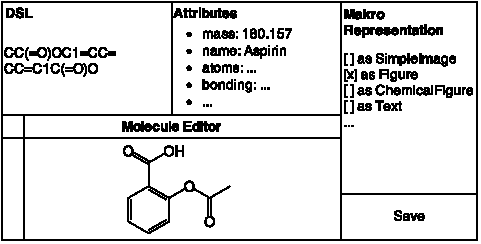
\includegraphics[width=1.45\textwidth]{figures/semanticeditor.svg.pdf} }
\caption{ Konzept für eine Weiterentwicklung des semantischen Editors für Dokumentelemente, anhand des Beispiels Chemiemolekül-Dokumentelement. }\label{semanticeditor}
\end{figure}
 
\subsection{Visionen neuer Ausbaustufen und Anwendungsfälle}\label{}
 
Ein Marktplatz für Dokumentelemente. Dort können Dokumentelemente z.B. als Software-Bibliotheken, oder direkt als SaaS via REST-Schnittstelle, zur Verfügung gestellt werden. Zur Konservierung und Wiederauffindbarkeit von Dokumentelementen, kann der Markplatz diese mit einem DOI (digital object identifier) versehen. Das kann auch als Geschäftsmodell dienlich sein: z.B. indem SaaS-Dokumentelemente, bei Laufzeit, Geld kosten. Oder Autoren können wie in einem App-Store Dokumentelemente durch einmaliges bezahlen zukaufen (Account/Firmagebunden), oder mit Bezahlung pro Dokument.

 
Positionierung als Open Access Platform, zum schreiben sowie publizieren von akademischen Werken. Dieser Dienst kann z.B. Dokumentelemente aus dem Marktplatz anbieten. Dokumentelemente können auch assistieren, z.B. ein Abschnitt kann abhängig von seinem Kontext selbständig nach Zitaten suchen und Werke, die mutmaßlich darin vorkommen, vorschlagen und diese auf Wunsch automatisch ins Literaturverzeichnis aufnehmen. Oder eine Art Typographie Lint, welches Warnungen herausgibt, falls bestimmte typografische Konventionen der gewählten Sprache mutmaßlich missachtet werden (z.B. falsche Anführungszeichen). Zudem können Autoren gegenseitig ihre Werke begutachten oder lektorieren. Ein Reputationssystem aus Zitaten und Begutachtungen kann besonders gute Gutachter herausheben. Ein Geschäftsmodell kann sein, dass Autoren bezahlte Gutachter oder Lektoren suchen bzw. beauftragen können und die Plattform erhält eine entsprechende Transaktionsgebühr pro Gutachten.

 
Erweiterte Autorenfunktionen. Ein Autor kann um das Dokument zugehörige Metadokumente aufbauen, wie beispielsweise Exzerpte. Aus diesen Exzerpten kann er direkt entsprechende Dokumentelemente in das Hauptdokument übernehmen. Ein kollaboratives Lektorat wird es vereinfachen, dass verschiedene Gutachter gleichzeitig zum Dokument Korrekturvorschläge und Kommentare einreichen.

 
Projektion von und in andere Formate, die Platform als Format-Zentrale. Quasi ein Reißwolf für Dokumente, es werden digitalisierte Handaufschriebe, Textdateien, PDFs etc. eingegeben; ein Klassifikator (der eventuell vom Dokumentelement direkt mitgeliefert wird) erkennt die verschiedenen Dokumentelemente die darin vorkommen. Der Autor bekommt vom System einen Gliederungsüberblick, der die aufgefunden Dokumentelemente anzeigt -- dadurch kann er sie bequem in sein Dokument einbauen. Beispiel: Ein Chemiker kann seine im Labor von Hand aufgeschriebenen Tabellen automatisch in ein Tabellen-Dokumentelement übersetzen lassen und dieses weiterverarbeiten. Auf diese Weise können auch historische Dokumente aufbereitet werden. Dadurch, dass das Dokument als abstrakter Syntaxbaum vorliegt, kann es in beliebige andere Formate transformiert werden. So könnte auch die Lektoratfunktion davon profitieren: Das Dokument wird z.B. in eine Word-Datei transformiert, der Lektor kann in seinem gewohnten Format Korrekturvorschläge machen; danach wird die annotierte Word-Datei in den Reißwolf gesteckt, dieser fusioniert die Korrekturvorschläge mit denen aus dem eigenen Lektorat. Ein Geschäftsmodell könnte sein: Die Benutzung des Reißwolfs kostet jeweils ein paar Cent, oder aufgefundene Dokumentelemente in das Dokument einzubauen kostet ein paar Cent.

 
Durch präzise definierte Dokumentklassen, kann der Editor dem Autor assistierend zur Seite stehen. Der Editor kann den Autor wie ein Sherpa durch die verschiedenen Vorgehensmodelle, die es bei der Erstellung von wissenschaftlicher Dokumentation zu beachten gibt, führen. So kann der Editor als ein Lernprogramm fungieren, welches die einzelnen Dokumententeile und ihre Bedeutungen erklärt und Tipps dazu gibt, welche Aussagen jeweils darin vorkommen sollten.

 
Durch Projektionen kann ein Dokument auf beliebige Art dargestellt werden. Es müssen auch nicht alle Bestandteile darin vorkommen oder können verkürzt dargestellt werden, oder mit zusätzlichen Anmerkungen versehen werden. Das ermöglicht es, dass der Dokumenteditor Strukturhilfen anbietet, wie z.B. eine Ansicht als Mindmap, zum schnellen Umstrukturieren des Dokuments. Oder auch die Anzeige aller im Dokument vorkommenden Fußnoten, zur schnellen Überprüfung, ob diese gut ausformuliert sind.

 
Modellierung von Dokumentelementen, durch schreiben eines einfachen Dokuments. Ein Autor verfasst ein (formales) Dokument, welches wiederum ein spezielles Dokumentelement beschreibt. Dieses Dokument dient quasi direkt als Modell für das Dokumentelement. Darin wird beschrieben welche Attribute vorkommen oder wie die Repräsentationen gestaltet sein sollen. Danach kann das dort beschriebene Dokumentelement in einem anderen Dokument verwendet werden. Eventuell kann dieser Vorgang mit Knowledge Discovery und durch Natural Language Programming verbessert werden, so dass sogar aus dem Text in natürlicher Sprache weitere Erkenntnisse über das Dokumentelement, bzw. dessen Modell, extrahiert werden können. Auf diese Art könnten Wissenschaftler ihre Modelle immer weiter verfeinern. Beispiel: Atommodelle. Es gäbe ein Dokument, welches formal das Teilchenmodell von Demokrit beschreibt. Resultat ist ein entsprechendes Dokumentelement. Dalton bezieht sich nun darauf bzw. verwendet in seinem Dokument das Demokrit-Modell und entwickelt es entsprechend weiter. Resultat seines Dokuments ist ein Dokumentelement mit dem Dalton-Modell. Es basiert nun sogar direkt auf dem Demokrit-Modell. Das ist mutmaßlich bis zum Orbitalmodell ausbaubar. Damit gäbe es eine formale semantische Verknüpfung zwischen den Modellen. Ob dies umsetzbar oder überhaupt nützlich ist, müsste jedoch erst noch geklärt werden.

 
\citep[S.~3]{Segaran} trifft es sehr präzise, wenn er behauptet, dass natürliche Sprache wohl die beste API für Wissen ist, die wir Menschen kennen. \citep[S.~1]{Knuth} hat dies in etwa auch so erkannt und daraus das programmiersprachenübergreifende Programmierparadigma des Literate Programming entwickelt. Dort soll Software wie ein Literaturwerk behandelt werden, d.h. Dokumentation und Programmcode werden in einer Datei simultan untergebracht. Die hier vorgestellten Konzepte eigenen sich mutmaßlich hervorragend, um Literate Programming umzusehen. Beispielsweise können einzelne größere Programmkomponenten wie z.B. ein For-Schleifen-Block auf spezielle Dokumentelemente abgebildet werden. Eine Funktionsdekleration wäre mit einem Kapitel vergleichbar, etc. Gemischt mit normalen Dokumentelementen, die beschreibend zur Seite stehen, könnte somit auch mit diesem System Literate Programming umgesetzt werden. Zudem kann jedes Programm-Dokumentelement eine passende Visualisierung von Datenstrukturen oder Programmflüssen darstellen. Durch den Modellcharakter der Dokumentelemente wäre es somit möglich, ein Programm sogar in verschiedene Programmiersprachen zu transformieren. Anwendungsfall: Ein DSL-Skript kann durch einen Wissenschaftler mit dem System programmiert, visualisiert und gleichzeitig dokumentiert werden kann.

